\documentclass[12pt, a4paper]{article}
\usepackage{enumerate,subfigure}
\usepackage{a4wide}
\usepackage{cite}
\usepackage[brazil]{babel}
\usepackage[T1]{fontenc}
\usepackage[utf8]{inputenc}
\usepackage{graphics}
\usepackage{graphicx}
\usepackage{url}
\usepackage{indentfirst}
\usepackage[mediumspace, mediumqspace, Grey, squaren]{SIunits} % Unidades SI
\usepackage{titlesec}
\usepackage{framed,color}
\usepackage[table,xcdraw]{xcolor}
\usepackage{multirow}
\usepackage{lscape}
\usepackage{scalefnt}
\usepackage{longtable}
\definecolor{shadecolor}{rgb}{0.75, 0.75, 0.75}


\setcounter{secnumdepth}{4}

\begin{document}

\title{  \vspace{-0.8in} 
\begin{figure}[!htb]
\centering
\includegraphics{imagens/brasao.png}
\end{figure}
 \Large  Minist\'erio da Educa\c{c}\~ao  \\
 Secretaria da Educa\c{c}\~ao Profissional e Tecnol\'ogica   \\
Instituto Federal de Educa\c{c}\~ao, Ci\^encia e Tecnologia da Para\'iba \\
Campus Guarabira\\
%MINISTÉRIO DA EDUCAÇÃO
%SECRETARIA DA EDUCAÇÃO PROFISSIONAL E TECNOLOGICA
%INSTITUTO FEDERAL DE EDUCAÇÃO, CIÊNCIA E TECNOLOGIA DA PARAÍBA
% Coordenação de Informática   \\ 
 %Grupo de Pesquisa em Redes de Computadores e Sistemas Distribuídos \\
 %Grupo de Pesquisa em Sistemas Digitais \\
\vspace{3cm}
\bf \large PROJETO PEDAG\'OGICO DE CURSO\\
\vspace{2cm}
\normalsize NOME DO CURSO:\\
\large Sistemas para Internet\\
\vspace{2cm}
\normalsize TIPO DO CURSO:\\
\large Superior de Tecnologia}


%\author{\vspace{2cm}\large Prof. Ruan Delgado Gomes, M.Sc.}
 \vspace{2cm}
\large
\date{\vspace{3.6cm}Guarabira, Setembro/2015}
\maketitle
\normalsize
\thispagestyle{empty}

\tableofcontents


%\newpage


%\thispagestyle{empty}
%\begin{center}
%\vspace*{3cm}
%\LARGE Proposta de Projeto \& Pesquisa \\ \vspace{3cm}
%      Experimentos para Identificação de Fontes de Interferência e Avaliação da Qualidade de Serviço de Redes de Sensores sem Fio em Ambientes Industriais \\  \vspace{5cm}
%{
%\normalsize
%        Ruan Delgado Gomes --- Aluno \\ \vspace{1cm}
%		  Marcelo Sampaio de Alencar --- Orientador \\
%			Iguatemi Eduardo Fonseca --- Co-orientador
%}
%\end{center}

%\newcommand{\HRule}{\rule{\linewidth}{1mm}}
%\HRule

\newpage
\normalsize
\pagenumbering{arabic}

%\input{apresentacao.tex}
\newpage
\section{Contexto da Institui\c{c}\~ao e do Curso}

\subsection{Contexto da Institui\c{c}\~ao}

\subsubsection{Dados da mantenedora}

% Please add the following required packages to your document preamble:
% \usepackage[table,xcdraw]{xcolor}
% If you use beamer only pass "xcolor=table" option, i.e. \documentclass[xcolor=table]{beamer}
\begin{table}[h]
\begin{tabular}{|
>{\columncolor[HTML]{C0C0C0}}l |
>{\columncolor[HTML]{FFFFFF}}l |
>{\columncolor[HTML]{FFFFFF}}l
>{\columncolor[HTML]{FFFFFF}}l
>{\columncolor[HTML]{FFFFFF}}l
>{\columncolor[HTML]{FFFFFF}}l |
>{\columncolor[HTML]{FFFFFF}}l |
>{\columncolor[HTML]{FFFFFF}}l |}
\hline
Mantenedora & \multicolumn{7}{l|}{\cellcolor[HTML]{FFFFFF}\begin{tabular}[c]{@{}l@{}}Instituto Federal de Educa\c{c}\~ao, Ci\^encia e Tecnologia\\ da Para\'iba - CNPJ - 10.783.898/0001-75\\ Pessoa Jurídica de Direito Público – Federal\end{tabular}}                                                            \\ \hline
Endereço    & \multicolumn{5}{l|}{\cellcolor[HTML]{FFFFFF}Avenida Primeiro de Maio}                                                                                                                                                                   & \cellcolor[HTML]{C0C0C0}Número:       & 720       \\ \hline
Bairro      & Jaguaribe                                      & \cellcolor[HTML]{C0C0C0}Cidade:                                     & João Pessoa                                              & \cellcolor[HTML]{C0C0C0}CEP:        & 58015-430       & \cellcolor[HTML]{C0C0C0}UF:           & PB        \\ \cline{1-3} \cline{5-8}
Telefone:   & \multicolumn{2}{l|}{\cellcolor[HTML]{FFFFFF}\begin{tabular}[c]{@{}l@{}}(83) 3208 3000\\ (83) 3208 3004\end{tabular}} & \multicolumn{1}{l|}{\cellcolor[HTML]{C0C0C0}Fax:}        & \multicolumn{4}{l|}{\cellcolor[HTML]{FFFFFF}(83) 3208 3088}                                               \\ \hline
E-mail:     & \multicolumn{7}{l|}{\cellcolor[HTML]{FFFFFF}ifpb@ifpb.edu.br}                                                                                                                                                                                                                               \\ \hline
Site:       & \multicolumn{7}{l|}{\cellcolor[HTML]{FFFFFF}www.ifpb.edu.br}                                                                                                                                                                                                                                \\ \hline
\end{tabular}
\end{table}

%colocar sub

\subsubsection{Dados da mantida}

% Please add the following required packages to your document preamble:
% \usepackage[table,xcdraw]{xcolor}
% If you use beamer only pass "xcolor=table" option, i.e. \documentclass[xcolor=table]{beamer}
\begin{table}[h]
\begin{tabular}{|
>{\columncolor[HTML]{C0C0C0}}l |
>{\columncolor[HTML]{FFFFFF}}l |
>{\columncolor[HTML]{FFFFFF}}l
>{\columncolor[HTML]{FFFFFF}}l
>{\columncolor[HTML]{FFFFFF}}l
>{\columncolor[HTML]{FFFFFF}}l |
>{\columncolor[HTML]{FFFFFF}}l |
>{\columncolor[HTML]{FFFFFF}}l |}
\hline
Mantida & \multicolumn{7}{l|}{\cellcolor[HTML]{FFFFFF}\begin{tabular}[c]{@{}l@{}}IFPB - Campus Guarabira\end{tabular}}                                                            \\ \hline
Endereço    & \multicolumn{5}{l|}{\cellcolor[HTML]{FFFFFF}Rua José Américo}                                                                                              & \cellcolor[HTML]{C0C0C0}Número: & s/n \\ \hline
Bairro      & Bairro Nordeste I     & \cellcolor[HTML]{C0C0C0}Cidade:     & Guarabira                                         & \cellcolor[HTML]{C0C0C0}CEP: & 58200-000 & \cellcolor[HTML]{C0C0C0}UF:     & PB  \\ \cline{1-3} \cline{5-8}
Telefone:   & \multicolumn{2}{l|}{\cellcolor[HTML]{FFFFFF}(83) 9188 0604} & \multicolumn{1}{l|}{\cellcolor[HTML]{C0C0C0}Fax:} & \multicolumn{4}{l|}{\cellcolor[HTML]{FFFFFF}}                                    \\ \hline
E-mail:     & \multicolumn{7}{l|}{\cellcolor[HTML]{FFFFFF}campus\_guarabira@ifpb.edu.br}                                                                                                                         \\ \hline
Site:       & \multicolumn{7}{l|}{\cellcolor[HTML]{FFFFFF}www.ifpb.edu.br}                                                                                                                                       \\ \hline
\end{tabular}
\end{table}


\subsubsection{Breve hist\'orico da institui\c{c}\~ao}

	O atual Instituto Federal de Educação Ciência e Tecnologia da Paraíba - IFPB tem mais de cem anos de existência. Ao longo de todo esse período, recebeu diferentes denominações (Escola de Aprendizes Artífices da Paraíba - de 1909 a 1937; Liceu Industrial de João Pessoa - de 1937 a 1961; Escola Industrial ``Coriolano de Medeiro'' ou Escola Industrial Federal da Paraíba - de 1961 a 1967; Escola Técnica Federal da Paraíba - de 1967 a 1999); Centro Federal de Educação Tecnológica da Paraíba – de 1999 a 2008 e, finalmente, IFPB, de 2008 aos dias atuais.

	Criado no ano de 1909, por meio de decreto presidencial de Nilo Peçanha, o seu perfil atendia a uma determinação contextual que vingava na época. Como Escola de Aprendizes Artífices, seu primeiro nome foi concebido para prover de mão de obra ao modesto parque industrial brasileiro que estava em fase de instalação.

	Àquela época, a Escola absorvia os chamados ``desvalidos da sorte'', pessoas desfavorecidas e até indigentes, que provocavam um aumento desordenado na população das cidades, notadamente com a expulsão de escravos das fazendas, que migravam para os centros urbanos. Tal fluxo migratório era mais um desdobramento social gerado pela abolição da escravatura, ocorrida em 1888, que desencadeava sérios problemas de urbanização.

	O IFPB, no início de sua história, assemelhava-se a um centro correcional, pelo rigor de sua ordem e disciplina. O decreto do Presidente Nilo Peçanha criou uma Escola de Aprendizes Artífices em cada capital dos estados da federação, mais com uma solução reparadora da conjuntura socioeconômica que marcava o período, para conter conflitos sociais e qualificar mão de obra barata, suprindo o processo de industrialização incipiente que, experimentando uma fase de implantação, viria a se intensificar a partir dos anos 30.

	A Escola da Paraíba, que oferecia os cursos de Alfaiataria, Marcenaria, Serralheria, Encadernação e Sapataria, inicialmente funcionou no Quartel do Batalhão da Polícia Militar do Estado, depois se transferiu para o Edifício construído na Avenida João da Mata, onde funcionou até os primeiros anos da década de 1960 e, finalmente, instalou-se no atual prédio localizado na Avenida Primeiro de Maio, bairro de Jaguaribe, em João Pessoa, Capital.

	Ainda como Escola Técnica Federal da Paraíba, no ano de 1995, a Instituição interiorizou suas atividades, por meio da instalação da Unidade de Ensino Descentralizada de Cajazeiras - UNED.

	Enquanto Centro Federal de Educação Tecnológica da Paraíba - CEFET-PB, a Instituição experimentou um fértil processo de crescimento e expansão em suas atividades, passando a contar, além de sua Unidade Sede, com o Núcleo de Educação Profissional - NEP, que funciona na Rua das Trincheiras.

	Desde então, o IFPB oferece à sociedade, paraibana e brasileira, cursos técnicos de nível médio (integrado e subsequente); cursos superiores de tecnologia, bacharelado e licenciatura, todos em consonância com a linha programática e princípios doutrinários consagrados na Lei de Diretrizes e Bases da Educação Nacional – LDB/EM e normas dela decorrentes.

	Como Centro Federal de Educação Tecnológica da Paraíba, ocorreu em 2007, a implantação da Unidade de Ensino Descentralizada de Campina Grande – UNED-CG e a criação do Núcleo de Ensino de Pesca, no município de Cabedelo.

	Com o advento da Lei 11.892/2008, o Instituto se consolida como uma instituição de referência da Educação Profissional na Paraíba. Além dos cursos, usualmente chamados de “regulares”, a Instituição também desenvolve um amplo trabalho de oferta de cursos extraordinários, de curta e média duração, atendendo a uma expressiva parcela da população, a quem são destinados também cursos técnicos básicos, programas de qualificação, profissionalização e reprofissionalização, para melhoria das habilidades de competência técnica no exercício da profissão.

	A Instituição, em obediência ainda às suas obrigações previstas em lei, tem desenvolvido estudos com vistas a oferecer programas para formação, habilitação e aperfeiçoamento de docentes da rede pública.

	Visando a ampliação de suas fronteiras de atuação, o Instituto desenvolve ações para atuar com competência na modalidade de Educação à Distância (EAD) e tem investido fortemente na capacitação dos seus professores e técnicos administrativos, no desenvolvimento de atividades de pós-graduação lato sensu, stricto sensu e de pesquisa aplicada, possibilitando as bases à oferta de pós-graduação nestes níveis, horizonte aberto com a nova Lei.

	Até o ano de 2010, contemplado com o Plano de Expansão da Educacional Profissional, Fase II, do Governo Federal, o Instituto implantou mais cinco Campi, no estado da Paraíba, contemplando cidades consideradas pólos de desenvolvimento regionais, como Picuí, Monteiro, Princesa Isabel, Patos e Cabedelo, al\'em de um n\'ucleo avan\c{c}ado na cidade de Guarabira. Associados aos Campi de Cajazeiras, Campina Grande, João Pessoa e Sousa (Escola Agrotécnica, que se incorporou ao antigo CEFET, proporcionando a criação do Instituto).

	Desta forma, o Instituto Federal da Paraíba abrange João Pessoa e Cabedelo, no litoral; Campina Grande no brejo e agreste; Picuí no Seridó Ocidental; Monteiro no Cariri; Patos, Cajazeiras, Souza e Princesa Isabel na região do sertão; Guarabira na Mesorregião da Mata Paraibana, mas politicamente está inserida no Brejo. O raio de abrangência dos campi é demonstrado na Figura~\ref{fig:IFPB1}.


\begin{figure}
       \centering
       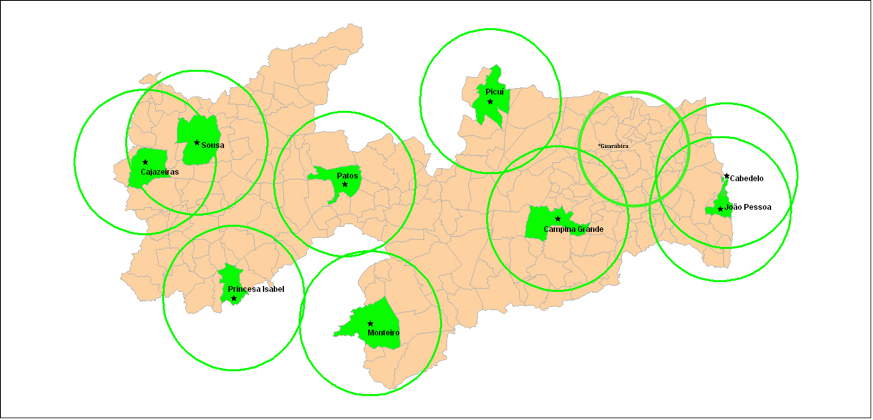
\includegraphics[height=2.5in]{imagens/campiIFPB1.png}
       \caption {Localização geográfica dos campi do IFPB no Estado da Paraíba.}
\label{fig:IFPB1}
\end{figure}


	As novas unidades educacionais levam Educação Profissional em todos os níveis (básico, técnico e tecnológico) oportunizando o desenvolvimento econômico e social e melhorando a qualidade de vida destas regiões.

	Vale ressaltar que a diversidade de cursos ora ofertados pela Instituição justifica-se em decorrência da experiência e tradição da mesma no tocante à educação profissional. O Instituto Federal da Paraíba, considerando as definições decorrentes da Lei n. 11.892/2009 e observando o contexto das mudanças estruturais que tem ocorrido na sociedade e na educação brasileira, adota um Projeto Acadêmico baseado na sua responsabilidade social, advinda da referida Lei, a partir da construção de um projeto pedagógico flexível, em consonância com o proposto na Lei de Diretrizes e Bases da Educação Nacional, buscando produzir e reproduzir os conhecimentos humanísticos, científicos e tecnológicos, de modo a proporcionar a formação plena da cidadania, que será traduzida na consolidação de uma sociedade mais justa e igual.

	O IFPB atua nas áreas profissionais das Ciências Agrárias, Ciências Biológicas, Ciências da Saúde, Ciências Exatas e da Terra, Ciências Humanas, Ciências Sociais Aplicadas, Engenharias, Linguística, Letras e Artes.

	São ofertados cursos nos eixos tecnológicos de Recursos Naturais, Produção Cultural e Design, Gestão e Negócios, Infraestrutura, Produção Alimentícia, Controle e Processos Industriais, Produção Industrial, Hospitalidade e Lazer, Informação e Comunicação, Ambiente, Saúde e Segurança.

	Nessa perspectiva, a organização do ensino no Instituto Federal da Paraíba oferece oportunidades em todos os níveis da aprendizagem, permitindo o processo de verticalização do ensino. Ampliado o cumprimento da sua responsabilidade social também atua fortemente desde Programas de Formação Continuada (FIC), PROEJA, Mulheres Mil, propiciando o prosseguimento de estudos por meio do Ensino Técnico de Nível Médio, Ensino Tecnológico de Nível Superior, as Licenciaturas, os Bacharelados e os estudos de Pós-Graduação Lato Sensu e Stricto Sensu.

	Além de desempenhar o seu próprio papel na qualificação e requalificação de recursos humanos, o IFPB atua no suporte tecnológico às diversas instituições de ensino, pesquisa e extensão, bem como no apoio às necessidades tecnológicas empresariais. Essa atuação não se restringe ao estado da Paraíba, mas gradativamente vem se consolidando dentro do contexto macrorregional delimitado pelos estados de Pernambuco, Ceará e Rio Grande do Norte.

	O Instituto Federal da Paraíba, em sintonia com o mercado de trabalho e com a expansão da Rede Federal de Educação Profissional, traça as estratégias para a implantação de 05 (cinco) novos campi nas cidades de Itaporanga, Itabaiana, Catolé do Rocha, Santa Rita e Esperança, contemplados no Plano de Expansão III. Assim, junto aos campi já existentes, os novos campi promover\~ao a interiorização da educação no território paraibano conforme Figura~\ref{fig:IFPB2}.


\begin{figure}
       \centering
       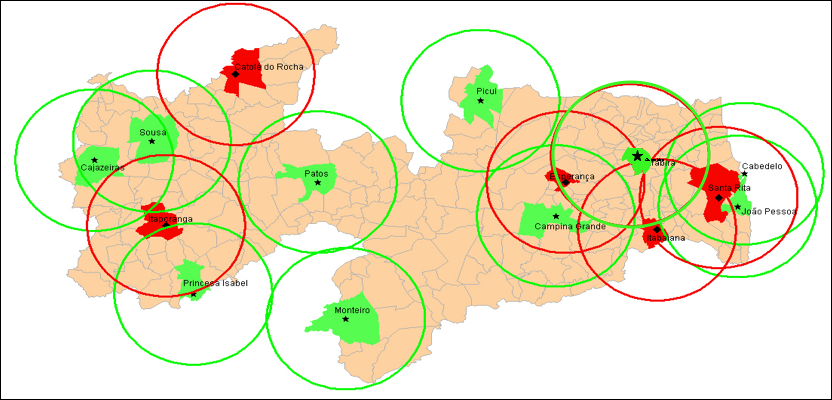
\includegraphics[height=2.5in]{imagens/campiIFPB2.png}
       \caption {Municípios paraibanos contemplados com o Plano de Expansão III do IFPB.}
\label{fig:IFPB2}
\end{figure}

\paragraph{S\'intese Hist\'orica do IFPB Campus Guarabira}\

	Guarabira foi a primeira cidade integrante do Plano de Expansão III a iniciar suas atividades educativas, portanto torna-se necessário discorrer sobre os aspectos e peculiaridades que a caracterizam.

	O IFPB Campus Guarabira foi inaugurado em 10 de outubro de 2011 (na \'epoca como N\'ucleo Avan\c{c}ado) e atualmente funciona na Rua José Américo de Almeida, S/N, no Bairro do Nordeste I, no Centro de Vocação Tecnológica - CVT (antigo CAIC).

	Os cursos ofertados pelo NAG - IFPB devem atender as carências da região, levando em consideração o contexto socioeconômico bem como sua viabilidade nessa fase inicial.

	Guarabira é um município que está localizado no Piemonte da Borborema, na microrregião que recebe o seu nome Microrregião de Guarabira. Seu nome, de origem tupi, quer dizer berço das garças, ``guará-pora'' ou ``bira'', isto é, moradia dos guarás. Com uma área de 149,50 $km^2$, o município ocupa o 115~{\degree} lugar em extensão territorial no Estado e possui uma posição geográfica invejável, pois fica a apenas 96 km de distância de João Pessoa (Capital Paraibana), 100 km de Campina Grande (maior cidade do interior nordestino), 199 km do Recife (Capital de Pernambuco e do Nordeste), 145 km de Natal (um dos maiores polos turísticos do Brasil) e a 230 km de Caruaru (grande centro comercial nordestino). A sede do município fica a 97 metros de altitude do nível do mar, tem sua posição geográfica determinada pelo paralelo 06~{\degree} 51’17" de latitude e 35~{\degree} 29’24" de longitude.

	É chamada Rainha do Brejo pelo fato de ser a principal cidade-polo de uma região que se caracteriza pela regularidade de chuvas. Guarabira é polo de educação na Região do Brejo, atendendo alunos do ensino fundamental até pós-graduação em ensino superior, situação que atrai estudantes de todo o estado da Paraíba, bem como de outros estados da federação.

	A cidade possui universidades privadas e públicas, incluindo o Campus III da Universidade Estadual da Paraíba - UEPB, contando com os cursos de Direito, História, Geografia, Letras e Pedagogia.

	A chegada do IFPB a Guarabira traz inovação e tecnologia, formando profissionais capacitados para atuarem diretamente no contexto econômico da região, ou seja, nos diversos setores: comércio, indústria e serviços; geograficamente, está localizada em uma região em que polariza mais de 30 cidades, todas tendo um forte vínculo com o município.

	Atualmente o Campus Guarabira oferta tr\^es cursos t\'ecnicos integrados ao ensino m\'edio: Inform\'atica, Edifica\c{c}\~oes e Contabilidade e o Curso Superior de Tecnologia em Gest\~ao Comercial. Com o progresso e o dinamismo presente nas capitais e principais cidades dos estados nordestinos, é primordial para a consolidação desta realidade, o desenvolvimento da educação por meio da formação de novos profissionais para atender a realidade local. Neste contexto, o Curso Superior de Tecnologia em Sistemas para Internet vem suprir demandas reais e urgentes neste cenário.

\subsubsection{Cen\'ario s\'ocio-econ\^omico da regi\~ao}

	A Paraíba está situada no Nordeste brasileiro, limitada pelos Estados de Pernambuco, Rio Grande do Norte e Ceará, além de ter sua costa banhada pelo Oceano Atlântico. Em 2013, contava com uma população estimada em 3.914.421 milhões de habitantes, segundo o Censo de 2010, divulgado pelo IBGE.

	Apesar de possuir uma economia pequena, se comparada com aquelas dos estados mais desenvolvidos do país, a Paraíba tem experimentado índices de crescimento bastante expressivos. A variação do Produto Interno Bruto deste Estado, em comparação aos índices apresentados para o Nordeste e o Brasil, pode ser vista com o auxílio do Quadro 3.

\begin{table}[h]
\caption{Produto Interno Bruto per capita do Brasil, Nordeste e Paraíba.}
\begin{tabular}{|
>{\columncolor[HTML]{FFFFFF}}l |
>{\columncolor[HTML]{FFFFFF}}l |
>{\columncolor[HTML]{FFFFFF}}l |
>{\columncolor[HTML]{FFFFFF}}l |
>{\columncolor[HTML]{FFFFFF}}l |}
\hline
\textbf{\begin{tabular}[c]{@{}l@{}}Ano Moeda\\ PIB per capita\end{tabular}} & \textbf{2008} & \textbf{2009} & \textbf{2010} & \textbf{2011} \\ \hline
Brasil                                                                      & 15.991,55     & 16.917,66     & 19.508,59     & 21.252,41     \\ \hline
Nordeste                                                                    & 7.485,55      & 8.167,75      & 9.561,41      & 10.379,55     \\ \hline
Paraíba                                                                     & 6.865,98      & 7.617,71      & 8.481,14      & 9.348,69      \\ \hline
\end{tabular}
\end{table}

	No tocante aos aspectos econômico, social e político, a Paraíba está dividida em 4 (quatro) mesorregiões, assim denominadas, de acordo com a classificação estabelecida pelo IBGE: Mata Paraibana, Agreste Paraibano, Borborema e Sertão Paraibano. Essas mesorregiões estão, por sua vez, desagregadas em 23 microrregiões geográficas. Diante da prevalência dos problemas enfrentados pela população que habita as áreas semi-áridas do estado e da necessidade de solucionar a crise econômica que afeta a Zona da Mata e a Região do Brejo, optou-se por adotar a divisão clássica do estado da Paraíba e agregar seus principais espaços econômicos nas seguintes zonas geoeconômicas: Litoral-Mata, Agreste-Brejo e Semi-Árida. A divisão das mesorregiões pode ser visto na Figura~\ref{fig:meso}.

\begin{figure}
       \centering
       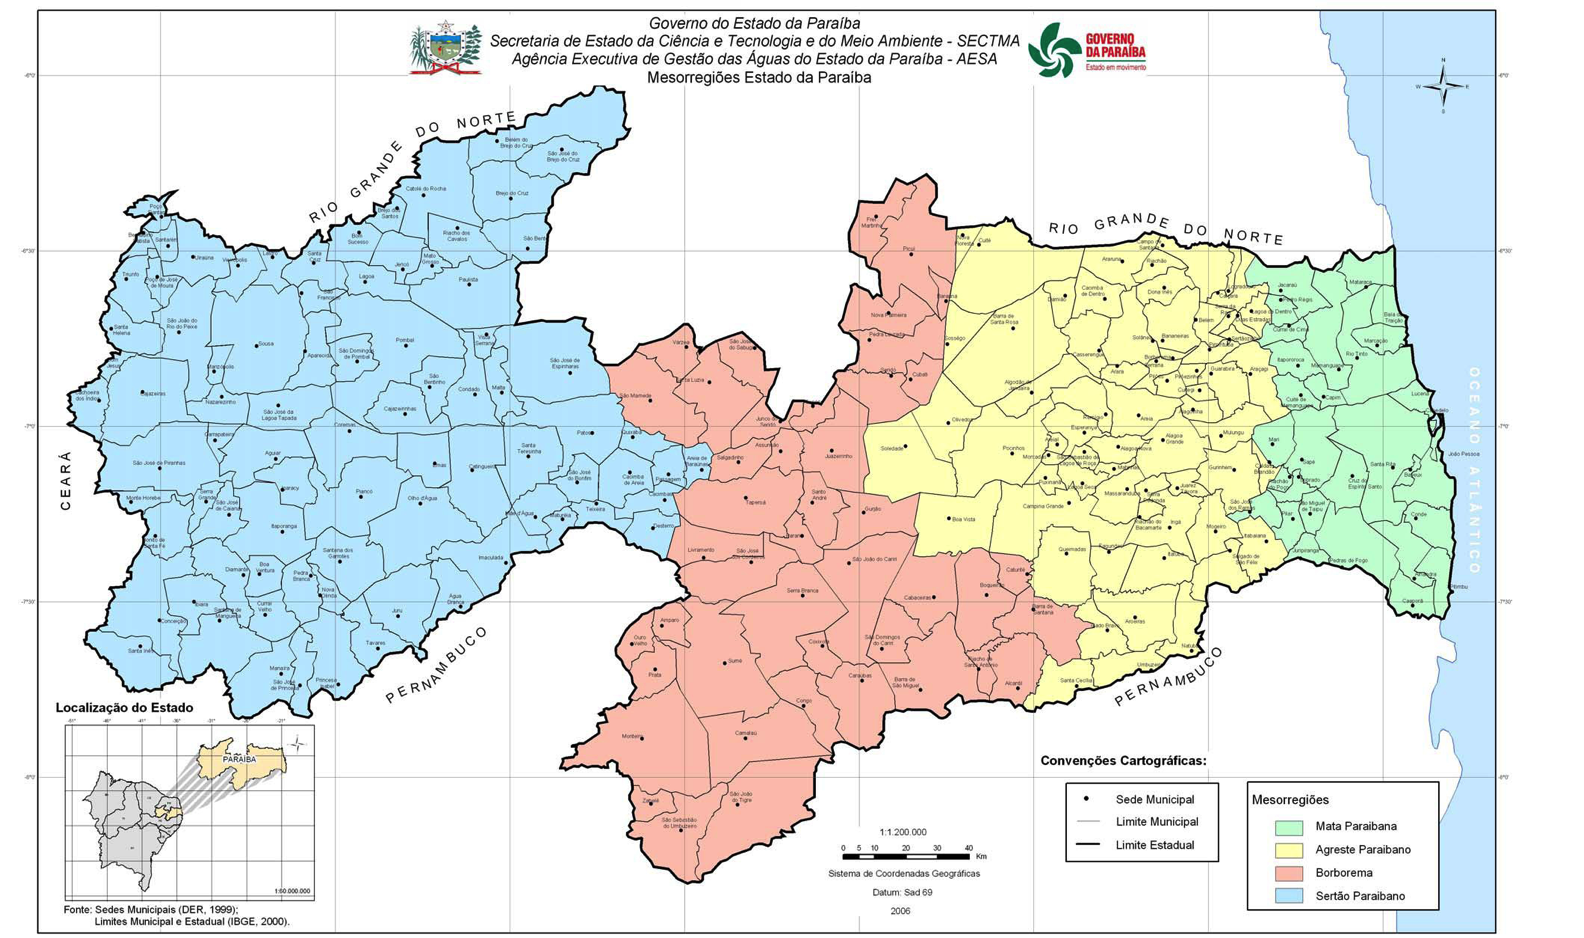
\includegraphics[height=3.0in]{imagens/mesorregioes.png}
       \caption { Mesorregiões econômicas da Paraíba. FONTE: PDI-IFPB (2010)}
\label{fig:meso}
\end{figure}


	A Zona Litoral-Mata corresponde à Mesorregião Mata Paraibana, definida pelo IBGE e integrada pelas seguintes Microrregiões Geográficas: Litoral Norte, Sapé, João Pessoa e Litoral Sul, que englobam 30 dos 223 municípios do Estado, ou seja, 13,45~\% do total. Com uma superfície de 5.242 $km^2$ (9,3~\% do território do Estado), em 2000 abrigava uma população de 1.196.594 habitantes, o que significa uma densidade de 228,3 $hab/km^2$. O grande aglomerado urbano da Capital do Estado é um dos principais responsáveis por essa concentração populacional.

	A Zona do Agreste-Brejo abrange quase que integralmente as Microrregiões constitutivas da Mesorregião do Agreste, tal como definida pelo IBGE: Esperança, Brejo Paraibano, Guarabira, Campina Grande, Itabaiana e Umbuzeiro. Essas seis microrregiões reúnem 48 municípios (21,5~\% do total). Para os efeitos da classificação aqui adotada, a Zona do Agreste-Brejo deixa de englobar as Microrregiões do Curimataú Ocidental e do Curimataú Oriental, que passam a integrar a Zona Semi-Árida. Com isto, a Zona do Agreste-Brejo passa a ter uma área de 7.684 $km^2$ (13,6~\% da superfície total do estado) e no ano de 2000 uma população de 950.494 habitantes (IDEME, 2001), consistindo em uma zona de grande concentração populacional, pois possuía, no referido ano, uma densidade demográfica de 123,7 $hab/km^2$, correspondendo a 54~\% da observada na Zona Litoral-Mata. A densidade demográfica do Agreste-Brejo é 2 vezes superior à média do Estado. O peso populacional do Agreste-Brejo é, em grande parte, devido à cidade de Campina Grande, onde vivem 37,4~\% dos habitantes dessa zona.

	A Zona Semi-Árida é a mais extensa em área, com 43.513,65 $km^2$ (77,1~\% do total do Estado), assim como a dotada de maior número absoluto de habitantes. Sua população, em 2000, era de 1.296.737 pessoas (37,6~\% do total), o que representava uma densidade demográfica de 29,8 $hab/km^2$. Esse indicador espelha as dificuldades enfrentadas pela população que vive naquela zona, pois dada à escassez relativa de recursos naturais que a caracteriza, ela apresenta a menor densidade demográfica entre as zonas geo-econômicas consideradas. Sua população está sujeita a condições de insustentabilidade, tanto econômica quanto social, bem mais difíceis de controlar do que as encontradas nas Zonas Litoral-Mata e Agreste-Brejo. Comparado aos demais espaços semi-áridos do Nordeste, o da Paraíba é um dos mais afetados pela degradação ambiental. Da categoria semiárida paraibana aqui considerada, fazem parte os seguintes espaços: Mesorregião do Sertão Paraibano (Microrregiões Geográficas de Catolé do Rocha, Cajazeiras, Sousa, Patos, Piancó, Itaporanga e Serra do Teixeira); Mesorregião da Borborema (Microrregiões do Seridó Ocidental, Seridó Oriental, Cariri Ocidental e Cariri Oriental); e as terras do Planalto da Borborema, conhecidas como Curimataú, representadas pelas Microrregiões do Curimataú Ocidental e do Curimataú Oriental, que integram a Mesorregião do Agreste, tal como classificada pelo IBGE.

	Para efeito de análise de mercado, podemos dividir a Paraíba em três mesorregiões distintas: a zona da mata, região polarizada pela capital João Pessoa; o agreste, região central do estado, polarizada pela cidade de Campina Grande e o sertão, com suas características próprias, polarizada pela cidade de Patos.

	O sertão se caracteriza pelo baixo índice de industrialização, em relação a sua extensão e densidade populacional. Basicamente, observam-se a presença de indústrias de beneficiamento mineral (área na qual o Estado apresenta um considerável potencial de exploração), além da indústria de alimentos e bebidas, ambas com baixos índices de automação. A mesorregião conta com três distritos industriais: Patos, com aproximadamente 35~ha; Sousa com 32,5~ha e Cajazeiras com 21,39~ha.

	Embora dotadas de razoável infraestrutura, as indústrias dessa mesorregião não declararam investimentos em melhorias ou ampliações da capacidade produtiva no protocolo de intenções industriais entre 1996 e 1998, e apenas uma delas recebeu incentivos do FAIM (Fundo de Apoio ao Desenvolvimento Industrial da Paraíba) no mesmo período, o que resultou em menos de 100 novas vagas de emprego na cidade de Cajazeiras.

	Na área educacional, o sertão paraibano é atendido pela Rede Estadual de Escolas Públicas, responsável pelo Ensino Médio, na maioria das cidades da região. A Rede Municipal é responsável pelo Ensino Básico e Fundamental, ofertado na zona urbana e rural da maioria dos municípios. A região conta ainda com dois campi do IFPB, em Sousa e Cajazeiras, que servem a boa parte da região do sertão, além de unidades do SENAI, SENAC, SEBRAE e rede privada, sendo também atendida por projetos do SENAR e do SENAT. No Ensino Superior, além do Campus de Cajazeiras, que oferta dois Cursos Superiores de Tecnologia (An\'alise e Desenvolvimento de Sistemas e Automação Industrial), um Curso Superior de Bacharelado em Engenharia Civil e um Curso Superior de Licenciatura em Matem\'atica, o sertão conta com vários campi da Universidade Federal de Campina Grande (UFCG), localizados nas cidades de Patos, Sousa e Cajazeiras, onde são oferecidos cursos como Engenharia Florestal, Veterinária, Direito, Pedagogia, entre outros. A cidade de Patos conta ainda com a Fundação Francisco Mascarenhas, que oferece cursos de graduação e pós-graduação.

	A mesorregião do agreste paraibano apresenta um grau de urbanização e desenvolvimento maior que a do sertão e comparável à zona da mata. Com três distritos industriais – todos situados na cidade de Campina Grande –, ela apresenta indústrias de transformação nas áreas de química, eletro-eletrônicos, mineração, têxtil, metal-mecânica, produtos alimentícios, bebidas, materiais plásticos, papel e papelão, cerâmica, couro calçado, editorial e gráfico e borracha. O índice de automação das indústrias varia de baixo a médio, com algumas indústrias empregando tecnologias de ponta no seu processo produtivo.

	Desta forma, Campina Grande, pólo da região, possui uma grande demanda de serviços técnicos na área de eletrônica e inform\'atica, seja para atender ao parque industrial, seja na prestação de serviços de manutenção ou desenvolvimento de equipamentos e sistemas. Observando o número de empresas assistidas pelos recursos do FAIM entre os anos de 1996 e 1998, cerca de 34 indústrias de diversos setores da economia foram beneficiadas, gerando cerca de 6.500 empregos somente nesta mesorregião.

	%Além do mais, o agreste, capitaneado por Campina Grande, conta com a presença de unidades do SENAI, SENAC, SEBRAE, além de outras instituições de educação profissional, públicas e privadas, tendo se destacado por sua vocação educacional, ampliando sua área de atendimento aos demais estados da região Nordeste e do país.

	Situação similar à do agreste ocorre na mesorregião da zona da mata. Os seis distritos industriais existentes nas cidades de João Pessoa, Conde, Alhandra, Guarabira, Santa Rita e Cabedelo abrigam indústrias nas mais diversas áreas da atividade econômica. O número de indústrias, volume de produção e taxas de emprego são os maiores do Estado, com maior concentração na área de João Pessoa, Bayeux, Santa Rita e Cabedelo.

	Na cidade de Guarabira, além da economia fortemente baseada no comércio, o setor industrial tem apresentado grande desenvolvimento nos últimos anos. Com um Distrito Industrial (administrado pela CINEP-Companhia de Desenvolvimento da Paraíba) em fase de expansão, e que há espaço e isenção fiscal para instalações de novas empresas. Podemos destacar as indústrias de:

\begin{itemize}

	\item Móveis de madeira e tubulares;
	\item Indústria de aguardente (Maribondo, Pinga do Norte e Jureminha);
	\item Indústria de sacos de nylon (Ráfia);
	\item Fábrica de calçados (chuteiras e calçados de couro);
	\item Indústrias cerâmica vermelha (filtros domésticos para água, telhas e tijolos);
	\item Indústrias de pré-moldados;
	\item Setor têxtil (Ricol, Vince e a Rotas fabricantes de fardamentos militares);
	\item Indústria de ração animal (ração para peixes e camarão);
	\item Abatedouro indústrial (produção de abate de 70.000 aves/dia);
	\item Ind\'ustria de produtos alimentícios (massas Frei Damião e Pão de Mel, O Ponto do Pão), além de distribuidoras de bebidas.

\end{itemize}

	%Embora o número de indústrias, bem como o volume de investimento tenha aumentado, a média de empregos na indústria tem decrescido nos últimos anos no Estado. Nota-se que, no mesmo período, houve um crescimento semelhante em outras áreas como a de serviços e comércio.

	No que diz respeito à oferta de educação básica, a região de Guarabira é atendida pelas Redes Estadual, Municipal e Privada. Guarabira tamb\'em disp\~oe de algumas faculdades privadas, como a Unopar, a Faluz e a Unilec, al\'em do Campus III da Universidade Estadual da Para\'iba.

	Devido \`a vocação da Para\'iba para o desenvolvimento de novas tecnologias nos campos da Engenharia Elétrica e de Informática, devido principalmente à influência da Universidade Federal de Campina Grande, em Campina Grande, observa-se o aumento do número de empresas de base tecnológica em Campina Grande, Jo\~ao Pessoa e empresas incubadas no Parque Tecnológico da Paraíba, que tem como sede da Federação das Indústrias do Estado, Campina Grande. Em Guarabira, algumas empresas que atuam na \'area de solu\c{c}\~oes em Tecnologia da Informa\c{c}\~ao e Comunica\c{c}\~ao t\^em surgido, como \'e o caso da empresa Show Tecnologia. Com a cria\c{c}\~ao do Curso Superior de Tecnologia em Sistemas para Internet no IFPB Guarabira, que ter\'a um forte foco empreendedor, espera-se que nos pr\'oximos anos novas empresas de tecnologia surjam na regi\~ao, permitindo a oferta de solu\c{c}\~oes e servi\c{c}os para as ind\'ustrias locais e para o forte com\'ercio da regi\~ao, al\'em da exporta\c{c}\~ao das solu\c{c}\~oes desenvolvidas para outras regi\~oes.

	%Na área educacional, destaca-se o número elevado de oferta de vagas nas instituições de ensino superior, bem como na educação básica e profissional. João Pessoa, a principal cidade da região, conta atualmente com onze IES – incluído o IFPB, centenas de escolas públicas e privadas que atuam na educação básica, além de unidades do SENAI, SENAC, SENAR, SENAT, SEBRAE e instituições privadas de educação profissional. Esta tornou-se um centro educacional de médio porte – em nível nacional – algo que tende cada vez mais a crescer em função da elevada demanda por oportunidades educacionais, tendência esta que tem merecido atenção e ações constantes do Instituto Federal da Paraíba, que conta com 3 unidades na região.

	O Plano de Desenvolvimento Sustentável do estado prevê investimentos em diversas áreas, levando em conta os seguintes fatores:

\begin{itemize}
	\item 	Potencialidades associadas aos complexos produtivos já instalados e consolidados como o: têxtil-vestuário, couro-calçados, eletroeletrônico, metal mecânico 	 	e mineração, indústria química e de alimentos, construção civil;
	\item 	Capacidade científica e tecnológica em segmentos específicos, em especial, agropecuária, eletroeletrônica e informática;
	\item 	Potencialidades representadas pelas pequenas e médias empresas;
	\item 	Boa dotação de Infraestrutura; a presença marcante de entidades voltadas para a formação, especialização e treinamento de recursos humanos, como centro de 		ensino superior, ao lado de entidades como SENAI, SENAC, IFPB e a ESPEP;
	\item 	Localização geográfica estratégica do Estado da Paraíba;
	\item 	Redução das desigualdades sociais;
	\item 	Desenvolvimento de programas estruturantes referenciados na sustentabilidade ambiental;
	\item 	Programas de saneamento e urbanização;
	\item 	Programa de incentivo ao turismo;
	\item 	Programa de recursos hídricos e de Polos de irrigação;
	\item 	Programa de incentivo ao desenvolvimento das cidades Polos: João Pessoa, Campina Grande, Guarabira, Monteiro, Patos, Pombal, Sousa e Cajazeiras;
	\item 	Programa de eixos de integração econômica (Rodovias, Ferrovias e Portos).
\end{itemize}

	O Instituto Federal de Educação, Ciência e Tecnologia da Paraíba abrange todo o território paraibano: João Pessoa e Cabedelo, no litoral; Campina Grande e Guarabira, no brejo e agreste; Picuí, no Seridó Ocidental; Monteiro, no Cariri; Patos, Cajazeiras, Sousa, CVT (Sousa) e Princesa Isabel, na região do sertão, conforme demonstrado na Figura 2. Atuando primordialmente na Paraíba, mas não excluindo atividades nacionais ou internacionais, o Instituto desenvolve atividades de ensino, pesquisa e extensão nas seguintes áreas: comércio, construção civil, educação, geomática, gestão, indústria, informática, letras, meio ambiente, química, recursos pesqueiros, agropecuária, saúde, telecomunicações e turismo, hospitalidade e lazer.

	Dessa forma, o IFPB procura, ao interiorizar a educação tecnológica, adequar sua oferta de ensino, extensão e pesquisa principalmente às necessidades estaduais. Ressalte-se que a localização geográfica da Paraíba permite que a área de influência do Instituto Federal se estenda além das divisas do estado. Assim, regiões mais industrializadas, como Recife e Natal, têm, historicamente, solicitado profissionais formados por este Instituto para suprir a demanda em áreas diversas.

	Portanto, além de desempenhar o seu próprio papel no desenvolvimento de pessoas, nos mais diversos níveis educacionais, o Instituto Federal da Paraíba atua em parceria com diversas instituições de ensino, pesquisa e extensão, no apoio às necessidades tecnológicas empresariais. Essa atuação não se restringe ao Estado da Paraíba, sendo gradualmente consolidada dentro do contexto macro regional, delimitado pelos Estados de Pernambuco, Paraíba e Rio Grande do Norte.

\subsubsection{Identidade Estratégica da IES}

\paragraph{Miss\~ao}\

	O IFPB tem como missão preparar profissionais cidadãos com sólida formação humanística e tecnológica para atuarem no mundo do trabalho e na construção de uma sociedade sustentável, justa e solidária, integrando o ensino, a pesquisa e a extensão.

\paragraph{Princ\'ipios institucionais}\

	No exercício da Gestão o IFPB deve garantir a todos os seus Campi a autonomia da Gestão Institucional democrática a partir de uma administração descentralizada tendo como referência os seguintes princípios:

\begin{itemize}
	\item Ética – Requisito básico orientador das ações institucionais;

	\item Desenvolvimento Humano – Desenvolver o ser humano, buscando sua integração à sociedade através do exercício da cidadania, promovendo o seu bem-estar social;

	\item Inovação – Buscar soluções às demandas apresentadas;

	\item Qualidade e Excelência – Promover a melhoria contínua dos serviços prestados.
\end{itemize}

\paragraph{Valores institucionais}\

\begin{itemize}
	\item Autonomia dos Campi – Administrar preservando e respeitando a singularidade de cada campus;
	\item Transparência – Disponibilizar mecanismos de acompanhamento e de conhecimento das ações da gestão, aproximando a administração da comunidade;
	\item Respeito – Atenção com alunos, servidores e público em geral;
	\item Compromisso Social – Participação efetiva nas ações sociais, cumprindo seu papel social de agente transformador da sociedade.
\end{itemize}

\paragraph{Visão de futuro}\

 O IFPB tem como visão de futuro a busca continua pelo reconhecimento nacional e internacional enquanto instituição de referência no campo da educação, da ciência e da tecnologia pela pratica do viés indissociável do ensino da pesquisa e da extensão. Enquanto uma instituição que trabalha cotidianamente para enfrentar os desafios apresentados pela sociedade tecnológica atual nos seus aspectos sociais, políticos, culturais e econômicos se transformando em um grande centro de referência científica e tecnológica capaz de indicar possíveis soluções para os problemas apresentados pelo poder público constituído e pelos setores da sociedade civil. Para ser essa referência no futuro o IFPB investe progressivamente de forma cont\'inua nos seguintes pontos:

\begin{itemize}
\item Otimiza\c{c}\~ao da expansão de mais campi, levando o conhecimento ao  maior número de pessoas possível no Estado da Paraíba;

\item Investimento na estrutura física da instituição, que permita criar espaços ergonômicos e pedagógicos que proporcionem as condições necessárias para o bom desenvolvimento do processo ensino-aprendizagem;

\item Investimento em cursos de licenciatura, bacharelado e de tecnologia;

\item Investimento na compra de equipamentos tecnológicos e simuladores que permitem aos alunos e professores a compreensão mais rápida dos conhecimentos práticos específicos relativos \~as diversas áreas profissionais;

\item Oferta de educação profissional e tecnológica, em todos os seus níveis e modalidades, formando e qualificando cidadãos com vistas na atuação profissional nos diversos setores da economia, com ênfase no desenvolvimento socioeconômico local, regional e nacional;

\item Desenvolvimento da educação profissional e tecnológica como processo educativo e investigativo de geração e adaptação de soluções técnicas e tecnológicas às demandas sociais e peculiaridades regionais;

\item Promo\c{c}\~ao da integração e da verticalização da educação básica à educação profissional e educação superior;

\item Orienta\c{c}\~ao da sua oferta formativa em benefício da consolidação e fortalecimento dos arranjos produtivos, sociais e culturais locais, identificados com base no mapeamento das potencialidades de desenvolvimento socioeconômico e cultural;

\item Desenvolvimento programas de extensão e de divulgação científica e tecnológica;

\item Est\'imulo ao desenvolvimento de espírito crítico e criativo;

\item Oferta de capacitação técnica e atualização pedagógica aos docentes das redes públicas de ensino;

\item desenvolvimento de programas de extensão e de divulgação científica e tecnológica;

\item Est\'imulo \`a pesquisa aplicada, \`a produção cultural, ao empreendedorismo, ao cooperativismo e ao desenvolvimento científico e tecnológico;

\item Promo\c{c}\~ao da produção, desenvolvimento e transferência de tecnologias sociais, notadamente as voltadas à preservação do meio ambiente e a melhoria da qualidade de vida;

\item Promo\c{c}\~ao da integração e correlação com instituições congêneres, nacionais e internacionais, com vista ao desenvolvimento e aperfeiçoamento de parcerias que levem a processos de ensino-aprendizagem, pesquisa e extensão;

\item Investimento em cursos de pós-graduação lato sensu de aperfeiçoamento e Especialização e em cursos de pós-graduação stricto sensu de mestrado e doutorado, que contribuam para promover o estabelecimento de bases sólidas em educação, ciência e tecnologia, com vistas no processo de geração e inovação tecnológica;

\item Estabelecimento de parcerias com o mundo produtivo e com setores da Sociedade.

\end{itemize}

\subsection{Contexto do Curso}


\subsubsection{Dados Gerais}

\begin{table}[h]
\begin{tabular}{|l|l|l|l|l|l|}
\hline
\textbf{Denominação do Curso}   & \multicolumn{5}{l|}{Tecnologia em Sistemas para Internet}                                                                                            \\ \hline
\textbf{Modalidade}             & \multicolumn{5}{l|}{Presencial}                                                                                                                 \\ \hline
\textbf{Endereço de Oferta}     & \multicolumn{5}{l|}{\begin{tabular}[c]{@{}l@{}}Rua José Américo, s/n, Bairro Nordeste I,\\ Guarabira-PB. Cep 58200-000\end{tabular}} \\ \hline
\multicolumn{6}{|c|}{\textbf{SITUAÇÃO LEGAL DO CURSO}}                                                                                                                            \\ \hline
                       & \multicolumn{2}{l|}{Autorização}                          & \multicolumn{3}{l|}{Reconhecimento}                                                 \\ \hline
Documento              & \multicolumn{2}{l|}{}                                     & \multicolumn{3}{l|}{}                                                               \\ \hline
N. Documento           & \multicolumn{2}{l|}{}                                     & \multicolumn{3}{l|}{}                                                               \\ \hline
Data Documento         & \multicolumn{2}{l|}{}                                     & \multicolumn{3}{l|}{}                                                               \\ \hline
Data da Publicação     & \multicolumn{2}{l|}{}                                     & \multicolumn{3}{l|}{}                                                               \\ \hline
N. Parecer/Despacho    & \multicolumn{2}{l|}{}                                     & \multicolumn{3}{l|}{}                                                               \\ \hline
Conceito MEC           & \multicolumn{2}{l|}{}                                     & \multicolumn{3}{l|}{}                                                               \\ \hline
\textbf{Turno de Funcionamento} & \textbf{Integral}                     & \textbf{Matutino}                   & \textbf{Vespertino}                   & \textbf{Noturno}                   & \textbf{Totais}                   \\ \hline
\textbf{Vagas anuais}           &                            &                            & 60                             &                           & 60                       \\ \hline
\textbf{Turmas Teóricas}        &                             &                            &  2                            &                           & 2                        \\ \hline
\textbf{Regime de Matrícula}    & \multicolumn{5}{l|}{Semestral por Disciplina}                                                                                                   \\ \hline
\end{tabular}
\end{table}


\subsubsection{Breve histórico do curso}

%O IFPB - Campus Guarabira tomou a decisão de oferecer o curso Superior de Tecnologia em Sistemas para Internet em Guarabira, tendo como base alguns fatores significativos, como por exemplo, a experiência positiva com o curso Técnico em Informática, a necessidade de forma\c{c}\~ao de mão de obra qualificada na área de Tecnologia da Informação e Comunicação (TIC) e principalmente por força das reivindicações feitas pelos próprios profissionais que fazem parte do quadro efetivo da instituição, pelos alunos e pela sociedade em geral.

%Além disso, outra motivação para a criação do curso foi o fortalecimento da área de informática no campus Guarabira. A existência do curso técnico na área de informática contribuiu de duas formas para a criação do curso superior. Primeiramente, oferece estrutura e recursos humanos para permitir o início do curso. Em segundo lugar, os alunos egressos dos cursos técnicos em informática terão oportunidade de continuar os estudos em nível superior sem precisar sair de Guarabira.

%Esse ponto, além de aumentar a demanda pelo curso, provavelmente aumentará o nível dos alunos ingressantes, já que espera-se que muitos alunos virão com conhecimentos adquiridos nos cursos técnicos. Por último, é interessante observar que o Campus de João Pessoa é a única instituição pública a ofertar tal curso na Paraíba e a demanda por profissionais dessa área vem crescendo significativamente. Guarabira, por ser a cidade mais importante comercialmente para a Microrregião do Brejo, só tem a ganhar com a criação do curso no Campus.

	O Curso Superior de Tecnologia em Sistemas para Internet do IFPB - Campus Guarabira iniciará suas atividades no primeiro semestre de 2016, ofertando 30 vagas, em regime de disciplinas, com acesso por meio do Sistema de Seleção Unificada (SISU) para os candidatos participantes do Exame Nacional de Ensino Médio (ENEM).

	Nessa perspectiva, o campus garante o acesso à formação profissional de qualidade com conhecimentos e habilidades necessárias para exercer atividades específicas no mercado de trabalho.


%Neste cenário, o IFPB autorizou a elaboração do Projeto Pedagógico do Curso. Assim, em DD de MÊS de 2014 a Direção Geral do Campus Guarabira emitiu a portaria GD NNNN, designando a comissão responsável pelos levantamentos acerca das necessidades para a estruturação e elaboração do projeto pedagógico do curso. A partir dai os docentes das áreas informática, de conhecimentos gerais e o setor pedagógico discutiram e aprovaram a matriz curricular para o curso de Tecnologia em Sistemas para Internet.

\newpage
\newpage
\section{Organiza\c{c}\~ao Did\'atico-Pedag\'ogica}

\subsection{Concep\c{c}\~ao do Curso}

A Paraíba está inserida há um bom tempo no circuito nacional e internacional de tecnologia de informação e comunicação, tendo como destaque a cidade de Campina Grande que apresenta na área tecnológica uma das molas do seu desenvolvimento. A cidade destaca-se na vocação da região no desenvolvimento de novas tecnologias no campo da Engenharia Elétrica e de Informática, devido principalmente à influência da UFCG, com seus Cursos de Engenharia Elétrica e Ciências da Computação, ambos classificados entre os melhores do país.

Como resultado dessa vocação, observa-se o aumento do número de empresas de base tecnológica e incubadas no Parque Tecnológico da Paraíba. Cabe ressaltar, entretanto, que, apesar desta posição de destaque, há uma carência na formação de profissionais qualificados, para serem absorvidos pelo pólo de tecnologia da região.

Pelo panorama apresentado, necessita-se formar profissionais de nível superior, preparados para enfrentar os novos desafios que surgem no mercado, capacitados para atuar nas diversas áreas tecnológicas. Além disso, deve-se buscar a formação humana, necessária à condução de projetos, agregando ao indivíduo o espírito criativo, essencial à inovação tão exigida no mundo competitivo de hoje. Ciente desta realidade e consciente do seu papel no contexto da educação brasileira, o Campus Guarabira do IFPB apresenta o Curso Superior de Tecnologia em Sistemas para Internet, entendendo que este é um espaço promissor no que tange à geração de emprego, atendendo às demandas da sociedade e ao desenvolvimento econômico da região.

O curso de Sistemas para Internet no Campus Guarabira do IFPB foi concebido com base nas recomendações do MEC, estando fundamentado nas habilidades, competências e conhecimentos necessários à formação, inovador, ciente de seu papel e responsabilidade na sociedade. Assim, o curso tem por objetivo formar um profissional que possua uma boa e sólida formação formação tecnológica, para garantir a sua inserção e competitividade no mercado de trabalho.

Para atender a esses pressupostos, na definição do Curso de Sistemas para Internet, considerou-se obter a formação de um profissional com características que atendessem à atual demanda do mercado de trabalho. Assim, esse curso propôs-se habilitar profissionais com conhecimentos nas áreas de Computação, Desenvolvimento de Software, Redes de Computadores e Sistemas Distribu\'idos para o desenvolvimento de soluções inovadoras em projetos de sistemas computacionais, principalmente voltados para tecnologias emergentes, como \'e o caso de tecnologias para a WEB e dispositivos m\'oveis. O Curso de Sistemas para Internet possui uma formação sólida nos fundamentos de Computação. O profissional em Sistemas para Internet estará habilitado para atuar em todas nas áreas em que os conhecimentos de computação são essenciais e complementares.  

O egresso do Curso de Sistemas para Internet receberá o conhecimento necessário para prosseguir em estudos de pós-graduação em razão do fundamentado conhecimento obtido nas disciplinas da área básica do curso e nas atividades realizadas em projetos de pesquisa e extensão que incentivam a busca por novos desafios.

\subsubsection{Justificativas do curso}

A expansão da computação é verificada pela quantidade e diversidade de sistemas computacionais utilizados em diferentes segmentos, seja no trabalho, na educação e entretenimento. No trabalho, estes sistemas têm sido empregados nas mais diversas áreas e finalidades: desde a automatização de fábricas à terapia ocupacional, sendo essenciais nas comunicações, fortemente presente na Internet e nos aplicativos web. No âmbito da educação, os referidos têm auxiliado, seja como suporte gerencial ou como ferramenta de apoio ao processo de ensino-aprendizagem. Na área de entretenimento, estão os jogos que utilizam as mais sofisticadas técnicas de projeto gráfico e conceitos como os de Inteligência Artificial. Fora esse contexto, existem diversos dispositivos, como os eletrodomésticos e aparelhos eletrônicos, com funcionalidades implementadas por meio de hardware e software.


O interesse pelo Curso de Sistemas para Internet vêm da necessidade de mão de obra qualificada na área de Tecnologia da Informação e Comunicação (TIC), como vem sendo noticiado constantemente pela imprensa. É importante também notar que o tecnólogo em Sistemas para Internet é capaz de prestar concurso para qualquer cargo de nível superior na área de TI, uma vez que esses concursos não restringem a formação apenas para bacharelado. Além disso, a Paraíba se destaca como grande formadora de mão de obra qualificada na área de TI, possuindo dois programas de pós-graduação, contando com dois cursos de mestrado e um de doutorado.%, o que facilita a captação de mão de obra qualificada para atuar no curso.

A expansão das Instituições de Ensino na área de informática ou computação, tem respaldo na exigência do mercado pelo aumento do número de profissionais e pelo desenvolvimento dessa área no País e no mundo. Guarabira est\'a localizada de forma privilegiada, a cerca de 100 km da capital Paraibana e a cerca de 90 km de Campina Grande, cidade que possui atua\c{c}\~ao destacada nas \'area de TIC, contando com um parque tecnol\'ogico e v\'arias empresas dessa \'area. O curso de tecnologia em Sistemas para Internet do IFPB - Campus Guarabira ser\'a o primeiro curso superior da \'area de inform\'atica a ser ofertado por uma institui\c{c}\~ao p\'ublica na região do brejo e o Campus Guarabira ser\'a o segundo campus a oferecer o curso em todo o IFPB (atualmente apenas o campus Jo\~ao Pessoa oferece esse curso).

O curso de Sistemas para Internet trabalha com tecnologias emergentes e que oferecem muitas oportunidades de emprego, como é o caso de desenvolvimento de software para web e desenvolvimento de aplicativos para dispositivos móveis. Além disso, a formação do profissional de TSI prevê um bom nível de conhecimento em redes de computadores, incluindo segurança de redes, áreas que também estão sendo demandadas pelo mercado de trabalho.

Outra motiva\c{c}\~ao para a criação do curso é o fortalecimento da área de informática no campus Guarabira, que já conta com dois cursos técnicos (um integrado e um subsequente). A existência do curso técnico na área de informática contribui de duas formas para a criação do curso superior. Primeiramente, oferece estrutura e recursos humanos para permitir o início do curso. Em segundo lugar, os alunos egressos dos cursos técnicos em informática terão oportunidade de continuar os estudos em nível superior sem precisar sair de Guarabira. Esse ponto, além de aumentar a demanda pelo curso, provavelmente aumentará o nível dos alunos ingressantes, já que espera-se que muitos alunos virão com conhecimentos adquiridos nos cursos técnicos. Por último, é interessante observar que o Campus de João Pessoa é a única instituição pública a ofertar tal curso na Paraíba e a demanda por profissionais dessa área vem crescendo significativamente. Guarabira, por ser a cidade mais importante comercialmente para a Microrregião do Brejo, só tem a ganhar com a criação do curso no Campus, já que é notório o crescimento do \textit{e-commerce} no Brasil. Para inserir a cidade nessa nova realidade são necessários profissionais do curso de Sistemas para Internet. %Além disso, há a possibilidade de interdisciplinaridade entre com o curso Tecnólogo em Gestão Comercial, pois mesmo sendo de áreas distintas, há uma convergência muito forte entre os dois cursos devido à vocação comercial da região.

	Outro aspecto a ser levado em consideração são as atividades já sendo desenvolvidas no campus Guarabira na área de informática. Um grande conjunto de atividades já foi desenvolvido e outro já está em andamento, envolvendo principalmente atividades de pesquisa. A seguir são listadas as atividades e projetos desenvolvidos pelos professores de informática nos últimos tr\^es anos:

\begin{itemize}
\item Criação do Grupo de Pesquisa em Redes de Computadores e Sistemas Distribuídos (GPRSD), liderado pelos professores Ruan Delgado Gomes e Erick Augusto Gomes de Melo. O grupo  conta atualmente com 7 (sete) pesquisadores do IFPB e da UFPB, e 7 (sete) alunos dos cursos técnicos em informática;

\item Aprovação no GPRSD no Edital 07/2012 - Programa de Apoio ao Fortalecimento dos Grupos de Pesquisa do IFPB;

\item Participação do GPRSD no projeto ``Forma-Engenharia - Desenvolvimento de Sistemas de Monitoramento e Controle de Motores de Indução Trifásicos''. Financiado pelo CNPq, por meio do edital da chamada CNPQ/VALE S.A. Nº 05/2012. Nesse projeto dois alunos do curso técnico subsequente em informática foram bolsistas de iniciação tecnológica e industrial – nível B do CNPq;

\item Participação do GPRSD no projeto ``Projeto Ver Brasil: Sistema Brasileiro de Exibição Digital'', financiado pelo Ministério da Cultura e Secretaria de Audiovisual em parceria com o Núcleo de Pesquisa LAViD, da UFPB. Nesse projeto um aluno do curso integrado em informática e um aluno do curso subsequente em informática foram bolsistas, além de três professores do campus da área de informática;

\item Criação do Grupo de Pesquisa em Sistemas Digitais (GPSDi), liderado pelos professores Otacílio de Araújo Ramos Neto e Ruan Delgado Gomes. O grupo conta atualmente com 2 (dois) pesquisadores e 7 (sete) alunos dos cursos Técnicos em Informática;

\item Aprovação do GPSDi na chamada MEC/SETEC/CNPq N º 94/2013 – Apoio a Projetos Cooperativos de Pesquisa Aplicada e de Extensão Tecnológica, com o projeto “Grupo de Estudos em Robótica Educacional”.  Nesse projeto, alunos do curso técnico integrado em informática estão se preparando para a olimpíada brasileira de robótica;

\item Participação no projeto ``Projeto Olímpico de Informática no IFPB'', financiado por meio da chamada MEC/SETEC/CNPq N º 94/2013 – Apoio a Projetos Cooperativos de Pesquisa Aplicada e de Extensão Tecnológica. Por meio desse projeto foram obtidas quatro medalhas na olimp\'iada paraibana de inform\'atica e uma men\c{c}\~ao honrosa na olim\'ipada brasileira de inform\'atica;

\item Aprovação do professor Ruan Delgado Gomes no edital 25-2013 Bolsa Pesquisador do IFPB, com o projeto intitulado “Desafios e Aplicações de Redes de Sensores sem Fio Industriais”;

\item Um total de 8 (quatro) bolsistas PIBIC-EM e 2 (dois) voluntários envolvidos em projetos de pesquisa aprovados nos editais de PIBIC-EM;

\item Aprovação no GPRSD no Edital 17/2014 - Programa de Apoio ao Fortalecimento dos Grupos de Pesquisa do IFPB;

\item Classifica\c{c}\~ao para a final do concurso de trabalhos t\'ecnicos em inform\'atica do evento Computer on the Beach 2015;

\item Foram publicados oito artigos em peri\'odico, oito artigos em anais de eventos e dois cap\'itulos de livro.

\end{itemize}

%Os resultados descritos demonstram o potencial do corpo docente e discente da \'area de inform\'atica do campus Guarabira.

%Quanto à vocação regional da cidade de Campina Grande, a computação está alicerçada nas empresas da área de informática existentes, incluindo as de consultoria em tecnologia de informação e comunicação, de desenvolvimento de soluções de hardware e software para diversos segmentos econômicos. No ano de 2001, edição de abril, a revista norte-americana, Newsweek, escolheu Campina Grande dentre as nove cidades de destaque no mundo que representam um novo modelo de centro tecnológico. Tal escolha não foi por acaso, tendo em vista que, atualmente existem doze indústrias voltadas a atividades de fabricação e serviços relacionados a informática com sede em Campina Grande, além de empresas de confecção de material eletrônico e equipamentos de comunicação.
%Essa vocação é sustentada por entidades e empresas que se agregam para fomentar e prover o desenvolvimento da área de tecnologia, destacando-se a fundação do Parque Tecnológico (PaqTcPB) e do Centro de Inovação Tecnológica Telmo Araújo (CITTA), que possui o objetivo de auxiliar na consolidação de novos negócios, incubando e apoiando as empresas que possuem ênfase em tecnologia e inovação durante os diversos estágios do negócio.
%O PaqTcPB, em 2013, possuía um total de 21 empresas incubadas, dessas, 15 são de Campina Grande. O CITTA está com uma previsão de investimento inicial de aproximadamente R$ 4 milhões e deverá sediar uma média de 50 empresas voltadas à produção de tecnologia. Esses números ilustram uma Campina Grande com perfil empreendedor, com projetos nas áreas de produção de software, geoprocessamento, setor eletroeletrônico e biotecnologia.

%colocar subtopicos

\subsubsection{Objetivos do curso}

\textbf{Geral}

\vspace{5mm}
Formar profissional capaz de atender as demandas da sociedade e do mercado de trabalho, contribuindo para a evolução do conhecimento do ponto de vista científico e tecnológico, aplicando-o na avaliação, especificação e desenvolvimento de ferramentas, métodos e sistemas computacionais. O curso prima pela formação humanística, respeitando princípios éticos, permitindo ao profissional a compreensão do mundo, com visão crítica e consistente do impacto da profissão de Sistemas para Internet na sociedade.

\vspace{5mm}
\textbf{Específicos}

\vspace{5mm}

De acordo com o cat\'alogo do MEC, o profissional formado no curso superior de Tecnologia em Sistemas para Internet, poder\'a ter as seguintes atribui\c{c}\~oes:

\begin{itemize}

\item atuar no desenvolvimento de programas, interfaces e aplicativos;
\item atuar nos ramos de com\'ercio e marketing eletr\^onicos;
\item atuar no desenvolvimento de p\'aginas e portais para internet e intranet;
\item atuar no gerenciamento de projetos de sistemas, inclusive com acesso a banco de dados;
\item atuar no desenvolvimento de projetos e aplica\c{c}\~oes para a rede mundial de computadores e na intergra\c{c}\~ao de m\'idias nas p\'aginas da internet;
\item atuar com tecnologias emergentes como: computa\c{c}\~ao m\'ovel, redes sem fio e sistemas distribu\'idos;
\item cuidar da implanta\c{c}\~ao, atualiza\c{c}\~ao, manuten\c{c}\~ao e seguran\c{c}a dos sistemas para internet.
\end{itemize}

Al\'em disso, o curso de Sistemas para Internet tem como objetivo formar profissionais que possam:

\begin{itemize}
\item Comunicar-se eficientemente nas formas escrita, oral e gráfica;
\item Atuar em equipes multidisciplinares;
\item Compreender e aplicar ética e responsabilidade profissional;
\item Estar preparado para necessidade de atualização profissional constante;
\item Assumir a postura de permanente busca de atualização profissional;
\end{itemize}

\subsection{Pol\'iticas Institucionais e sua Correla\c{c}\~ao com o Curso}

        Atualmente o Campus Guarabira, em observância às suas obrigações previstas em lei, oferece Cursos Técnicos Integrados ao Ensino Médio, Cursos Técnicos Subsequentes e um Curso Superior de Tecnologia, todos em consonância com os princípios doutrinários consagrados na Lei de Diretrizes e Bases da Educação Nacional – LDBEN. 

        No Campus Guarabira existem dois cursos técnicos na \'area de inform\'atica, sendo um integrado e outro subsequente. Desta forma, com o objetivo de expandir a verticalização do ensino no Campus e em consonância com as políticas institucionais constantes no Plano de Desenvolvimento Institucional do IFPB, foi proposto o Curso de Tecnologia em Sistemas para Internet, com o objetivo de formar profissionais qualificados para atuarem no mercado de trabalho, bem como, capazes de prosseguirem seus estudos na pós-graduação. 


\subsection{Organiza\c{c}\~ao Curricular}

	A organização curricular do curso observa as determinações legais presentes na Lei de Diretrizes e Bases da Educação Nacional (LDBEN no. 9.394/96), no Decreto no 5.154/2004, na Resolução CNE/CP no 03/2002 e no Catálogo Nacional de Cursos Superiores de Tecnologia. Esses referenciais norteiam as instituições formadoras, definem o perfil, a atuação e os requisitos básicos necessários à formação profissional do Tecnólogo em Sistemas para Internet, quando estabelece competências e habilidades, conteúdos curriculares, prática profissional, bem como os procedimentos de organização e funcionamento dos cursos.

	Os cursos superiores de tecnologia possuem uma estrutura curricular fundamentada na concepção de eixos tecnológicos constantes do Catálogo Nacional de Cursos Superiores de Tecnologia (CNCST), instituído pela Portaria MEC no. 10/2006. Trata-se de uma concepção curricular que favorece o desenvolvimento de práticas pedagógicas integradoras e articula o conceito de trabalho, ciência, tecnologia e cultura, à medida que os eixos tecnológicos se constituem de agrupamentos dos fundamentos científicos comuns, de intervenções na natureza, de processos produtivos e culturais, além de aplicações científicas às atividades humanas.

	A proposta pedagógica do curso está organizada por núcleos politécnicos os quais favorecem a prática da interdisciplinaridade, apontando para o reconhecimento da necessidade de uma educação profissional e tecnológica integradora de conhecimentos científicos e experiências e saberes advindos do mundo do trabalho, e possibilitando, assim, a construção do pensamento tecnológico crítico e a capacidade de intervir em situações concretas.

	Essa proposta possibilita a realização de práticas interdisciplinares, concernente a conhecimentos científicos e tecnológicos, propostas metodológicas, tempos e espaços de formação.

	Desse modo, a matriz curricular dos cursos de graduação tecnológica organiza-se em dois núcleos, o núcleo fundamental e o núcleo científico e tecnológico. O núcleo fundamental compreende conhecimentos científicos imprescindíveis ao desempenho acadêmico dos ingressantes. Contempla, ainda, revisão de conhecimentos da formação geral, objetivando construir base científica para a formação tecnológica. Nesse núcleo, há dois propósitos pedagógicos indispensáveis: o domínio da língua portuguesa e, de acordo com as necessidades do curso, a apropriação dos conceitos científicos básicos.

	O núcleo científico e tecnológico compreende disciplinas destinadas à caracterização da identidade do profissional tecnólogo. Compõe-se por uma unidade básica (relativa a conhecimentos de formação científica para o ensino superior e de formação tecnológica básica) e por uma unidade tecnológica (relativa à formação tecnológica específica, de acordo com a área do curso). Essa última unidade contempla conhecimentos intrínsecos à área do curso, conhecimentos necessários à integração curricular e conhecimentos imprescindíveis à formação específica.

	A matriz curricular do curso está organizada por disciplinas em regime de crédito, com período semestral, com 2.XXX horas destinadas às disciplinas que compõem os núcleos politécnicos, YY horas destinadas a seminários curriculares e ZZZ horas destinadas à prática profissional, totalizando a carga horária de 2.PPP horas.

\newpage
\subsubsection{Estrutura curricular}
%\vspace{-1mm}
\begin{table}[h]
\tiny
\centering
\begin{tabular}{llll}
\hline
\rowcolor[HTML]{34CDF9} 
\multicolumn{4}{|c|}{\cellcolor[HTML]{34CDF9}\textbf{Primeiro Período}}                                                                                                                                                                                          \\ \hline
\rowcolor[HTML]{34CDF9} 
\multicolumn{1}{|l|}{\cellcolor[HTML]{34CDF9}\textbf{Disciplinas}} & \multicolumn{1}{l|}{\cellcolor[HTML]{34CDF9}\textbf{Teórica}} & \multicolumn{1}{l|}{\cellcolor[HTML]{34CDF9}\textbf{Prática}} & \multicolumn{1}{l|}{\cellcolor[HTML]{34CDF9}\textbf{Total}} \\ \hline
\multicolumn{1}{|l|}{Inglês Instrumental}                          & \multicolumn{1}{l|}{67}                                       & \multicolumn{1}{l|}{}                                         & \multicolumn{1}{l|}{67}                                     \\ \hline
\multicolumn{1}{|l|}{Fundamentos de Redes de Computadores}         & \multicolumn{1}{l|}{47}                                       & \multicolumn{1}{l|}{20}                                       & \multicolumn{1}{l|}{67}                                     \\ \hline
\multicolumn{1}{|l|}{Cálculo Diferencial e Integral}               & \multicolumn{1}{l|}{100}                                      & \multicolumn{1}{l|}{}                                         & \multicolumn{1}{l|}{100}                                    \\ \hline
\multicolumn{1}{|l|}{Algoritmos e Lógica de Programação}           & \multicolumn{1}{l|}{50}                                       & \multicolumn{1}{l|}{50}                                       & \multicolumn{1}{l|}{100}                                    \\ \hline
\multicolumn{1}{|l|}{Fundamentos da Computação}                    & \multicolumn{1}{l|}{20}                                       & \multicolumn{1}{l|}{13}                                       & \multicolumn{1}{l|}{33}                                     \\ \hline
\multicolumn{1}{|l|}{Linguagens de Marcação}                       & \multicolumn{1}{l|}{30}                                       & \multicolumn{1}{l|}{20}                                       & \multicolumn{1}{l|}{50}                                     \\ \hline
\rowcolor[HTML]{34CDF9} 
\multicolumn{1}{|r|}{\cellcolor[HTML]{34CDF9}\textbf{Subtotal}}    & \multicolumn{1}{l|}{\cellcolor[HTML]{34CDF9}\textbf{314}}     & \multicolumn{1}{l|}{\cellcolor[HTML]
{34CDF9}\textbf{103}}     & \multicolumn{1}{l|}{\cellcolor[HTML]{34CDF9}\textbf{417}}   \\ \hline
\multicolumn{4}{l}{}                                                                                                                                                                                                                                             \\ \hline
\rowcolor[HTML]{34CDF9} 
\multicolumn{4}{|c|}{\cellcolor[HTML]{34CDF9}\textbf{Segundo Período}}                                                                                                                                                                                          \\ \hline
\rowcolor[HTML]{34CDF9} 
\multicolumn{1}{|l|}{\cellcolor[HTML]{34CDF9}\textbf{Disciplinas}} & \multicolumn{1}{l|}{\cellcolor[HTML]{34CDF9}\textbf{Teórica}} & \multicolumn{1}{l|}{\cellcolor[HTML]{34CDF9}\textbf{Prática}} & \multicolumn{1}{l|}{\cellcolor[HTML]{34CDF9}\textbf{Total}} \\ \hline
\multicolumn{1}{|l|}{Português Instrumental}                          & \multicolumn{1}{l|}{67}                                       & \multicolumn{1}{l|}{}                                         & \multicolumn{1}{l|}{67}                                     \\ \hline
\multicolumn{1}{|l|}{Protocolos de Interconexão de Redes}         & \multicolumn{1}{l|}{47}                                       & \multicolumn{1}{l|}{20}                                       & \multicolumn{1}{l|}{67}                                     \\ \hline
\multicolumn{1}{|l|}{Estruturas de Dados I}               & \multicolumn{1}{l|}{37}                                      & \multicolumn{1}{l|}{30}                                         & \multicolumn{1}{l|}{67}                                    \\ \hline
\multicolumn{1}{|l|}{Probabilidade e Estatística}           & \multicolumn{1}{l|}{70}                                       & \multicolumn{1}{l|}{13}                                       & \multicolumn{1}{l|}{83}                                    \\ \hline
\multicolumn{1}{|l|}{Arquitetura de Computadores}                    & \multicolumn{1}{l|}{40}                                       & \multicolumn{1}{l|}{27}                                       & \multicolumn{1}{l|}{67}                                     \\ \hline
\multicolumn{1}{|l|}{Linguagens de Script}                       & \multicolumn{1}{l|}{30}                                       & \multicolumn{1}{l|}{20}                                       & \multicolumn{1}{l|}{50}                                     \\ \hline
\rowcolor[HTML]{34CDF9} 
\multicolumn{1}{|r|}{\cellcolor[HTML]{34CDF9}\textbf{Subtotal}}    & \multicolumn{1}{l|}{\cellcolor[HTML]{34CDF9}\textbf{291}}     & \multicolumn{1}{l|}{\cellcolor[HTML]
{34CDF9}\textbf{110}}     & \multicolumn{1}{l|}{\cellcolor[HTML]{34CDF9}\textbf{401}}   \\ \hline
\multicolumn{4}{l}{}                                                                                                                                                                                                                                             \\ \hline
\rowcolor[HTML]{34CDF9} 
\multicolumn{4}{|c|}{\cellcolor[HTML]{34CDF9}\textbf{Terceiro Período}}                                                                                                                                                                                          \\ \hline
\rowcolor[HTML]{34CDF9} 
\multicolumn{1}{|l|}{\cellcolor[HTML]{34CDF9}\textbf{Disciplinas}} & \multicolumn{1}{l|}{\cellcolor[HTML]{34CDF9}\textbf{Teórica}} & \multicolumn{1}{l|}{\cellcolor[HTML]{34CDF9}\textbf{Prática}} & \multicolumn{1}{l|}{\cellcolor[HTML]{34CDF9}\textbf{Total}} \\ \hline
\multicolumn{1}{|l|}{Interação Humano-Computador}                          & \multicolumn{1}{l|}{50}                                       & \multicolumn{1}{l|}{17}                                         & \multicolumn{1}{l|}{67}                                     \\ \hline
\multicolumn{1}{|l|}{Bancos de Dados I}         & \multicolumn{1}{l|}{40}                                       & \multicolumn{1}{l|}{27}                                       & \multicolumn{1}{l|}{67}                                     \\ \hline
\multicolumn{1}{|l|}{Estruturas de Dados II}               & \multicolumn{1}{l|}{37}                                      & \multicolumn{1}{l|}{30}                                         & \multicolumn{1}{l|}{67}                                    \\ \hline
\multicolumn{1}{|l|}{Sistemas Operacionais}           & \multicolumn{1}{l|}{47}                                       & \multicolumn{1}{l|}{20}                                       & \multicolumn{1}{l|}{67}                                    \\ \hline
\multicolumn{1}{|l|}{Metodologia da Pesquisa Científica}                    & \multicolumn{1}{l|}{20}                                       & \multicolumn{1}{l|}{13}                                       & \multicolumn{1}{l|}{33}                                     \\ \hline
\multicolumn{1}{|l|}{Programação Orientada a Objetos}                       & \multicolumn{1}{l|}{50}                                       & \multicolumn{1}{l|}{33}                                       & \multicolumn{1}{l|}{83}                                     \\ \hline
\rowcolor[HTML]{34CDF9} 
\multicolumn{1}{|r|}{\cellcolor[HTML]{34CDF9}\textbf{Subtotal}}    & \multicolumn{1}{l|}{\cellcolor[HTML]{34CDF9}\textbf{244}}     & \multicolumn{1}{l|}{\cellcolor[HTML]
{34CDF9}\textbf{140}}     & \multicolumn{1}{l|}{\cellcolor[HTML]{34CDF9}\textbf{384}}   \\ \hline
\multicolumn{4}{l}{}                                                                                                                                                                                                                                             \\ \hline
\rowcolor[HTML]{34CDF9} 
\multicolumn{4}{|c|}{\cellcolor[HTML]{34CDF9}\textbf{Quarto Período}}                                                                                                                                                                                          \\ \hline
\rowcolor[HTML]{34CDF9} 
\multicolumn{1}{|l|}{\cellcolor[HTML]{34CDF9}\textbf{Disciplinas}} & \multicolumn{1}{l|}{\cellcolor[HTML]{34CDF9}\textbf{Teórica}} & \multicolumn{1}{l|}{\cellcolor[HTML]{34CDF9}\textbf{Prática}} & \multicolumn{1}{l|}{\cellcolor[HTML]{34CDF9}\textbf{Total}} \\ \hline
\multicolumn{1}{|l|}{Programação para a Web I}                          & \multicolumn{1}{l|}{43}                                       & \multicolumn{1}{l|}{40}                                         & \multicolumn{1}{l|}{83}                                     \\ \hline
\multicolumn{1}{|l|}{Fundamentos de Economia}         & \multicolumn{1}{l|}{50}                                       & \multicolumn{1}{l|}{}                                       & \multicolumn{1}{l|}{50}                                     \\ \hline
\multicolumn{1}{|l|}{Segurança da Informação}               & \multicolumn{1}{l|}{47}                                      & \multicolumn{1}{l|}{20}                                         & \multicolumn{1}{l|}{67}                                    \\ \hline
\multicolumn{1}{|l|}{Programação Paralela e Distribuída}           & \multicolumn{1}{l|}{37}                                       & \multicolumn{1}{l|}{30}                                       & \multicolumn{1}{l|}{67}                                    \\ \hline
\multicolumn{1}{|l|}{Bancos de Dados II}                    & \multicolumn{1}{l|}{40}                                       & \multicolumn{1}{l|}{27}                                       & \multicolumn{1}{l|}{67}                                     \\ \hline
\multicolumn{1}{|l|}{Análise e Projeto de Sistemas}                       & \multicolumn{1}{l|}{50}                                       & \multicolumn{1}{l|}{17}                                       & \multicolumn{1}{l|}{67}                                     \\ \hline
\rowcolor[HTML]{34CDF9} 
\multicolumn{1}{|r|}{\cellcolor[HTML]{34CDF9}\textbf{Subtotal}}    & \multicolumn{1}{l|}{\cellcolor[HTML]{34CDF9}\textbf{267}}     & \multicolumn{1}{l|}{\cellcolor[HTML]
{34CDF9}\textbf{134}}     & \multicolumn{1}{l|}{\cellcolor[HTML]{34CDF9}\textbf{401}}   \\ \hline
\multicolumn{4}{l}{}                                                                                                                                                                                                                                             \\ \hline
\rowcolor[HTML]{34CDF9} 
\multicolumn{4}{|c|}{\cellcolor[HTML]{34CDF9}\textbf{Quinto Período}}                                                                                                                                                                                          \\ \hline
\rowcolor[HTML]{34CDF9} 
\multicolumn{1}{|l|}{\cellcolor[HTML]{34CDF9}\textbf{Disciplinas}} & \multicolumn{1}{l|}{\cellcolor[HTML]{34CDF9}\textbf{Teórica}} & \multicolumn{1}{l|}{\cellcolor[HTML]{34CDF9}\textbf{Prática}} & \multicolumn{1}{l|}{\cellcolor[HTML]{34CDF9}\textbf{Total}} \\ \hline
\multicolumn{1}{|l|}{Programação para a Web II}                          & \multicolumn{1}{l|}{43}                                       & \multicolumn{1}{l|}{40}                                         & \multicolumn{1}{l|}{83}                                     \\ \hline
\multicolumn{1}{|l|}{Padrões de Projeto de Software}         & \multicolumn{1}{l|}{37}                                       & \multicolumn{1}{l|}{30}                                       & \multicolumn{1}{l|}{67}                                     \\ \hline
\multicolumn{1}{|l|}{Gerência e Configuração de Serviços para a Internet}               & \multicolumn{1}{l|}{30}                                      & \multicolumn{1}{l|}{37}                                         & \multicolumn{1}{l|}{67}                                    \\ \hline
\multicolumn{1}{|l|}{Engenharia de Software}           & \multicolumn{1}{l|}{50}                                       & \multicolumn{1}{l|}{17}                                       & \multicolumn{1}{l|}{67}                                    \\ \hline
\multicolumn{1}{|l|}{Programação para Dispositivos Móveis}                    & \multicolumn{1}{l|}{37}                                       & \multicolumn{1}{l|}{30}                                       & \multicolumn{1}{l|}{67}                                     \\ \hline
\multicolumn{1}{|l|}{Empreendedorismo em Software}                       & \multicolumn{1}{l|}{50}                                       & \multicolumn{1}{l|}{17}                                       & \multicolumn{1}{l|}{67}                                     \\ \hline
\rowcolor[HTML]{34CDF9} 
\multicolumn{1}{|r|}{\cellcolor[HTML]{34CDF9}\textbf{Subtotal}}    & \multicolumn{1}{l|}{\cellcolor[HTML]{34CDF9}\textbf{247}}     & \multicolumn{1}{l|}{\cellcolor[HTML]
{34CDF9}\textbf{171}}     & \multicolumn{1}{l|}{\cellcolor[HTML]{34CDF9}\textbf{418}}   \\ \hline
\multicolumn{4}{l}{}                                                                                                                                                                                                                                             \\ \hline
\rowcolor[HTML]{34CDF9} 
\multicolumn{4}{|c|}{\cellcolor[HTML]{34CDF9}\textbf{Sexto Período}}                                                                                                                                                                                          \\ \hline
\rowcolor[HTML]{34CDF9} 
\multicolumn{1}{|l|}{\cellcolor[HTML]{34CDF9}\textbf{Disciplinas}} & \multicolumn{1}{l|}{\cellcolor[HTML]{34CDF9}\textbf{Teórica}} & \multicolumn{1}{l|}{\cellcolor[HTML]{34CDF9}\textbf{Prática}} & \multicolumn{1}{l|}{\cellcolor[HTML]{34CDF9}\textbf{Total}} \\ \hline
\multicolumn{1}{|l|}{Sistemas Distribuídos}                          & \multicolumn{1}{l|}{47}                                       & \multicolumn{1}{l|}{20}                                         & \multicolumn{1}{l|}{67}                                     \\ \hline
\multicolumn{1}{|l|}{Comércio Eletrônico}         & \multicolumn{1}{l|}{33}                                       & \multicolumn{1}{l|}{}                                       & \multicolumn{1}{l|}{33}                                     \\ \hline
\multicolumn{1}{|l|}{Desenvolvimento de Aplicações Corporativas}               & \multicolumn{1}{l|}{37}                                      & \multicolumn{1}{l|}{30}                                         & \multicolumn{1}{l|}{67}                                    \\ \hline
\multicolumn{1}{|l|}{Projeto em TSI}                    & \multicolumn{1}{l|}{10}                                       & \multicolumn{1}{l|}{57}                                         & \multicolumn{1}{l|}{67}                                    \\ \hline
\multicolumn{1}{|l|}{Tópicos Especiais}                       & \multicolumn{1}{l|}{67}                                       & \multicolumn{1}{l|}{}                                        & \multicolumn{1}{l|}{67}                                     \\ \hline
\multicolumn{1}{|l|}{TCC}                       & \multicolumn{1}{l|}{10}                                       & \multicolumn{1}{l|}{57}                                       & \multicolumn{1}{l|}{67}                                     \\ \hline
\rowcolor[HTML]{34CDF9} 
\multicolumn{1}{|r|}{\cellcolor[HTML]{34CDF9}\textbf{Subtotal}}    & \multicolumn{1}{l|}{\cellcolor[HTML]{34CDF9}\textbf{204}}     & \multicolumn{1}{l|}{\cellcolor[HTML]
{34CDF9}\textbf{164}}     & \multicolumn{1}{l|}{\cellcolor[HTML]{34CDF9}\textbf{368}}   \\ \hline
\multicolumn{4}{l}{}                                                                                                                                                                                                                                            
\end{tabular}
\end{table}

\newpage

\begin{landscape}

\subsubsection{Fluxograma}

% Please add the following required packages to your document preamble:
% \usepackage[table,xcdraw]{xcolor}
% If you use beamer only pass "xcolor=table" option, i.e. \documentclass[xcolor=table]{beamer}
\begin{table}[h]
\scalefont{0.5}
\begin{tabular}{|c|c|c|c|c|c|}
\hline
\rowcolor[HTML]{9B9B9B} 
\textbf{\unit{1}{\degree} Período}                                                                                    & \textbf{\unit{2}{\degree} Período}                                                                                   & \textbf{\unit{3}{\degree} Período}                                                            & \textbf{\unit{4}{\degree} Período}                                                           & \textbf{\unit{5}{\degree} Período}                                                                               & \textbf{\unit{6}{\degree} Período}                         \\ \hline
\rowcolor[HTML]{EFEFEF} 
Inglês Instrumental                                                                                   & Português Instrumental                                                                               & Interação Humano-Computador                                                   & Programação para a Web I                                                     & Programação para a Web II                                                                        & Sistemas Distribuídos                      \\ \hline
\rowcolor[HTML]{C0C0C0} 
{\color[HTML]{333333} \begin{tabular}[c]{@{}c@{}}Fundamentos de Redes\\ de Computadores\end{tabular}} & {\color[HTML]{333333} \begin{tabular}[c]{@{}c@{}}Protocolos de Interconexão\\ de Redes\end{tabular}} & {\color[HTML]{333333} Banco de Dados I}                                       & {\color[HTML]{333333} Fundamentos de Economia}                               & {\color[HTML]{333333} \begin{tabular}[c]{@{}c@{}}Padrões de Projeto de \\ Software\end{tabular}} & {\color[HTML]{333333} Comércio Eletrônico} \\ \hline
\rowcolor[HTML]{EFEFEF} 
Cálculo Diferencial e Integral                                                                        & Estrutura de Dados I                                                                                 & Estrutura de Dados II                                                         & Segurança da Informação                                                      & \begin{tabular}[c]{@{}c@{}}Gerência e Configuração \\ de Serviços para a Internet\end{tabular}   & Desenvolvimento de Aplicações Corporativas \\ \hline
\rowcolor[HTML]{C0C0C0} 
\begin{tabular}[c]{@{}c@{}}Algoritmos e Lógica de \\ Programação\end{tabular}                         & Probabilidade e Estatística                                                                          & Sistemas Operacionais                                                         & \begin{tabular}[c]{@{}c@{}}Programação Paralela e\\ Distribuída\end{tabular} & Engenharia de Software                                                                           & Projeto em TSI                             \\ \hline
\rowcolor[HTML]{EFEFEF} 
Fundamentos da Computação                                                                             & Arquitetura de Computadores                                                                          & \begin{tabular}[c]{@{}c@{}}Metodologia da Pesquisa \\ Científica\end{tabular} & Banco de Dados II                                                            & \begin{tabular}[c]{@{}c@{}}Programação para Dispositivos\\ Móveis\end{tabular}                   & Tópicos Especiais                          \\ \hline
\rowcolor[HTML]{C0C0C0} 
Linguagens de Marcação                                                                                & Linguagens de Script                                                                                 & \begin{tabular}[c]{@{}c@{}}Programação Orientada a \\ Objetos\end{tabular}    & Análise e Projeto de Sistemas                                                & \begin{tabular}[c]{@{}c@{}}Empreendedorismo em\\ Software\end{tabular}                           & TCC                                        \\ \hline
\end{tabular}
\end{table}

\end{landscape}

%\newpage

\subsubsection{Ementário e Bibliografia}

\paragraph{Estruturas de Dados I}

%PREENCHER DADOS DA DISCIPLINA A SEGUIR
%\vspace{-12mm}
\begin{center}\textbf{Dados do Componente Curricular}\end{center}
\vspace{-5mm}
\noindent\rule{16.5cm}{0.4pt}
\\
\textbf{Nome:} Estruturas de Dados I
\\ 
\textbf{Curso:} Tecnologia em Sistemas para Internet
\\ 
\textbf{Período:} \unit{2}{\degree}
\\ 
\textbf{Carga Horária:} \unit{67}{\hour}
\\ 
\textbf{Docente Responsável:} Otacílio de Araújo Ramos Neto
\\ 
\noindent\rule{16.5cm}{0.4pt}\\
\\
%PREENCHER A EMENTA A SEGUIR
\vspace{-12mm}
\begin{center}\textbf{Ementa}\end{center}
\vspace{-5mm}
\noindent\rule{16.5cm}{0.4pt}
\\
Conceitos básicos, crescimento de funções e recorrências; Algoritmos de ordenação e busca; Estruturas de dados elementares; Árvores de busca binária.\\ 
\noindent\rule{16.5cm}{0.4pt}\\
\\
%PREENCHER OS OBJETIVOS A SEGUIR
\vspace{-12mm}
\begin{center}\textbf{Objetivos}\end{center}
\vspace{-5mm}
\noindent\rule{16.5cm}{0.4pt}
\\
\begin{itemize}
\item Apresentar os conceitos básicos para criação e análise de algoritmos;
\item Apresentar os algoritmos básicos de ordenação e busca;
\item Capacitar os alunos a utilizarem as estruturas de dados elementares em problemas reais;
\item Apresentar aos alunos as árvores de busca binária e capacitá-los no seu uso.
\end{itemize} 
\noindent\rule{16.5cm}{0.4pt}\\
\\
%PREENCHER OS CONTEUDOS PROGRAMATICOS A SEGUIR (CUIDADO PARA NAO DEIXAR A TABELA MUITO GRANDE)
\vspace{-12mm}
\begin{center}\textbf{Conteúdo Programático}\end{center}
\vspace{-5mm}
\noindent\rule{16.5cm}{0.4pt}
\\
\begin{itemize}
 \item \textbf{Conceitos básicos:} Análise e projeto de algoritmos; Notação assintótica; O Método da Substituição, Método da Árvore de Recursão e Método Mestre.
 \item \textbf{Algoritmos de ordenação e busca:} Ordenação por inserção, Heapsort, Quicksort e ordenação em tempo linear; Busca sequencial e busca binária.
 \item \textbf{Estruturas de dados elementares:} Implementações de ponteiros e objetos; Pilhas, filas e listas ligadas.
 \item \textbf{Árvores de pesquisa binária:} Conceitos fundamentais de árvores de pesquisa binária; Algoritmos de inserção, remoção e busca; Impressão \textit{In-Order}, \textit{Post-Order} e \textit{Pre-Order} .
\end{itemize}
\noindent\rule{16.5cm}{0.4pt}\\
\\
%COLOCAR A METODOLOGIA DE ENSINO A SEGUIR
\vspace{-12mm}
\begin{center}\textbf{Metodologia de Ensino}\end{center} 
\vspace{-5mm}
\noindent\rule{16.5cm}{0.4pt}
\\
   Aulas expositivas utilizando recursos audiovisuais e quadro, além de aulas práticas utilizando computadores. Adicionalmente, serão realizadas atividades práticas individuais ou em grupo, para consolidação do conteúdo ministrado.\\
\noindent\rule{16.5cm}{0.4pt}\\
\\
%COLOCAR AVALIACAO DO PROCESSO DE ENSINO E APRENDIZAGEM A SEGUIR
\vspace{-12mm}
\begin{center}\textbf{Avaliação do Processo de Ensino e Apendizagem}\end{center}
\vspace{-5mm}
\noindent\rule{16.5cm}{0.4pt}
\\
   Avaliações escritas. Avalia\c{c}\~oes pr\'aticas envolvendo a resolu\c{c}\~ao de problemas computacionais.\\
\noindent\rule{16.5cm}{0.4pt}\\
\\
%PREENCHER RECURSOS NECESSARIOS A SEGUIR
\vspace{-12mm}
\begin{center}\textbf{Recursos Necessários}\end{center}
\vspace{-5mm}
\noindent\rule{16.5cm}{0.4pt}
\\
\begin{itemize} 
  \item Listas de Exercícios;
  \item Livros e apostilas;
  \item Utilização de recursos da web;
  \item Quadro branco;
  \item Marcadores para quadro branco;
  \item Sala de aula com acesso à internet, microcomputador e TV ou projetor para apresentação de slides ou material multimídia;
  \item Laboratório de microcomputadores contendo componentes de hardware e software específicos;
\end{itemize}
\noindent\rule{16.5cm}{0.4pt}\\ - 
\\
%PREENCHER BIBLIOGRAFIA A SEGUIR
\vspace{-12mm}
\begin{center}\textbf{Bibliografia}\end{center}
\vspace{-5mm}
\noindent\rule{16.5cm}{0.4pt}
\\
\begin{itemize} 
  \item Básica:
	\begin{enumerate}
	\item CELES, Waldemar. Introdução a Estrutura de Dados -  ISBN 978-85-3521-228-0, Editora Campus Elsevier, 2004.
	\item T.H. Cormen, C.E. Leiserson, R.L. Rivest, C. Stein, "Algoritmos - Teoria e Prática", 3a. ed., ISBN: 8535236996, Editora Campus, 2012.
	\item TENENBAUM, Aaron M. LANGSAM, Yedidyah. AUGENSTEIN, Moshe J. Estrutura de Dados Usando C - ISBN 8534603480, Makron Books. 
	
	\end{enumerate}
  \item Complementar:
	\begin{enumerate} 
	\item Steven S Skiena, The Algorithm Design Manual, Springer; 2nd edition, ISBN: 978-1849967204, 2008.\\
	\end{enumerate}
\end{itemize}
\noindent\rule{16.5cm}{0.4pt}\\
\\

\clearpage
\paragraph{Fundamentos da Computa\c{c}\~ao}

%PREENCHER DADOS DA DISCIPLINA A SEGUIR
%\vspace{-12mm}
\begin{center}\textbf{Dados do Componente Curricular}\end{center}
\vspace{-5mm}
\noindent\rule{16.5cm}{0.4pt}
\\
\textbf{Nome:} Fundamentos da Computa\c{c}\~ao
\\ 
\textbf{Curso:} Tecnologia em Sistemas para Internet
\\ 
\textbf{Período:} \unit{1}{\degree}
\\ 
\textbf{Carga Horária:} \unit{33}{\hour}
\\ 
\textbf{Docente Responsável:} Ruan Delgado Gomes
\\ 
\noindent\rule{16.5cm}{0.4pt}\\
\\
%PREENCHER A EMENTA A SEGUIR
\vspace{-12mm}
\begin{center}\textbf{Ementa}\end{center}
\vspace{-5mm}
\noindent\rule{16.5cm}{0.4pt}
\\
Conceitos introdut\'orios de inform\'atica; Representa\c{c}\~ao de dados e convers\~ao de base; Opera\c{c}\~oes aritm\'eticas com n\'umeros bin\'arios; L\'ogica digital; T\'opicos especiais em computa\c{c}\~ao.\\
\noindent\rule{16.5cm}{0.4pt}\\
\\
%PREENCHER OS OBJETIVOS A SEGUIR
\vspace{-12mm}
\begin{center}\textbf{Objetivos}\end{center}
\vspace{-5mm}
\noindent\rule{16.5cm}{0.4pt}
\\
\begin{itemize}
\item Apresentar os conceitos de \textit{hardware} e \textit{software};
\item Apresentar a representação digital de dados e informação;
\item Introduzir conceitos de l\'ogica;
\item Apresentar o funcionamento das portas lógicas;
\item Apresentar as tecnologias e aplicações de computadores.
\end{itemize} 
\noindent\rule{16.5cm}{0.4pt}\\
\\
%PREENCHER OS CONTEUDOS PROGRAMATICOS A SEGUIR (CUIDADO PARA NAO DEIXAR A TABELA MUITO GRANDE)
\vspace{-12mm}
\begin{center}\textbf{Conteúdo Programático}\end{center}
\vspace{-5mm}
\noindent\rule{16.5cm}{0.4pt}
\\
\begin{itemize}

 \item \textbf{Conceitos introdut\'orios de inform\'atica:} Histórico e evolução dos computadores; Defini\c{c}\~oes de \textit{software} e \textit{hardware}; Modelo conceitual da arquitetura de organiza\c{c}\~ao de um computador; Classifica\c{c}\~ao dos computadores; Perif\'ericos de entrada e sa\'ida.

 \item \textbf{Representa\c{c}\~ao de dados e convers\~ao de base:} Representação de dados; Representação de números inteiros na base binária; Representação de números inteiros na base octal; Representação de números inteiros nas base hexadecimal; Convers\~ao de bases.

 \item \textbf{Opera\c{c}\~oes aritm\'eticas com n\'umeros bin\'arios:} Opera\c{c}\~oes aritm\'eticas b\'asicas com n\'umeros bin\'arios.

 \item \textbf{L\'ogica digital:} Introdu\c{c}\~ao \`a l\'ogica; L\'ogica digital; Portas l\'ogicas; Constru\c{c}\~ao de circuitos combinacionais simples.

 \item \textbf{T\'opicos especiais em computa\c{c}\~ao:} Conte\'udo vari\'avel, envolvendo temas relevantes e atuais da computa\c{c}\~ao.

\end{itemize}
\noindent\rule{16.5cm}{0.4pt}\\
\\
%COLOCAR A METODOLOGIA DE ENSINO A SEGUIR
\vspace{-12mm}
\begin{center}\textbf{Metodologia de Ensino}\end{center} 
\vspace{-5mm}
\noindent\rule{16.5cm}{0.4pt}
\\
   Aulas expositivas utilizando recursos audiovisuais e quadro, além de aulas práticas utilizando computadores. Adicionalmente, serão realizadas atividades práticas individuais ou em grupo, para consolidação do conteúdo ministrado.\\
\noindent\rule{16.5cm}{0.4pt}\\
\\
%COLOCAR AVALIACAO DO PROCESSO DE ENSINO E APRENDIZAGEM A SEGUIR
\vspace{-12mm}
\begin{center}\textbf{Avaliação do Processo de Ensino e Apendizagem}\end{center}
\vspace{-5mm}
\noindent\rule{16.5cm}{0.4pt}
\\
   Avaliações escritas e pr\'aticas\\
\noindent\rule{16.5cm}{0.4pt}\\
\\
%PREENCHER RECURSOS NECESSARIOS A SEGUIR
\vspace{-12mm}
\begin{center}\textbf{Recursos Necessários}\end{center}
\vspace{-5mm}
\noindent\rule{16.5cm}{0.4pt}
\\
\begin{itemize} 
  \item Listas de Exercícios;
  \item Livros e apostilas;
  \item Utilização de recursos da web;
  \item Quadro branco;
  \item Marcadores para quadro branco;
  \item Sala de aula com acesso à internet, microcomputador e TV ou projetor para apresentação de slides ou material multimídia;
  \item Laboratório de microcomputadores contendo componentes de hardware e software específicos;
\end{itemize}
\noindent\rule{16.5cm}{0.4pt}\\
\\
%PREENCHER BIBLIOGRAFIA A SEGUIR
\vspace{-12mm}
\begin{center}\textbf{Bibliografia}\end{center}
\vspace{-5mm}
\noindent\rule{16.5cm}{0.4pt}
\\
\begin{itemize} 
  \item Básica:
	\begin{enumerate}
	\item MONTEIRO, M. A. Introdução à Organização de Computadores. ISBN: 9788521615439. Editora LTC. 5 Ed., 2007; 
	\item IDOETA, I. V.; CAPUANO, F. G. Elementos de Eletrônica Digital. ISBN: 8571940193. Editora Érica, 40 Ed., 2007;
	\item VELLOSO, F. C. Informática: Conceitos Básicos. ISBN: 9788535243970. Editora Campus, 8 Ed., 2011. 
	\end{enumerate}
  \item Complementar:
	\begin{enumerate} 
	\item TANENBAUM, Andrew S. Organização Estruturada de Computadores. ISBN: 9788581435398. Editora Pearson. 6 Ed., 2013.
	\end{enumerate}
\end{itemize}
\noindent\rule{16.5cm}{0.4pt}\\
\\

\clearpage
\paragraph{Algoritmos e L\'ogica de Programa\c{c}\~ao}

%PREENCHER DADOS DA DISCIPLINA A SEGUIR
%\vspace{-12mm}
\begin{center}\textbf{Dados do Componente Curricular}\end{center}
\vspace{-5mm}
\noindent\rule{16.5cm}{0.4pt}
\\
\textbf{Nome:} Algoritmos e L\'ogica de Programa\c{c}\~ao
\\ 
\textbf{Curso:} Tecnologia em Sistemas para Internet
\\ 
\textbf{Período:} \unit{1}{\degree}
\\ 
\textbf{Carga Horária:} \unit{100}{\hour}
\\ 
\textbf{Docente Responsável:} Ruan Delgado Gomes
\\ 
\noindent\rule{16.5cm}{0.4pt}\\
\\
%PREENCHER A EMENTA A SEGUIR
\vspace{-12mm}
\begin{center}\textbf{Ementa}\end{center}
\vspace{-5mm}
\noindent\rule{16.5cm}{0.4pt}
\\
Conceito de Algoritmos e Linguagens de Programação; Estruturas de Decisão; Estruturas de Repetição; Vetores e Matrizes; Manipulação de Strings; Modularização; Recursividade; Registros (Estruturas).\\
\noindent\rule{16.5cm}{0.4pt}\\
\\
%PREENCHER OS OBJETIVOS A SEGUIR
\vspace{-12mm}
\begin{center}\textbf{Objetivos}\end{center}
\vspace{-5mm}
\noindent\rule{16.5cm}{0.4pt}
\\
\begin{itemize}
\item Saber construir programas de computador obedecendo aos princípios da programação estruturada;
\item Conhecer conceitos básicos relacionados à construção de algoritmos;
\item Compreender e elaborar estruturas de controle;
\item Saber manipular dados por meio de Strings, Vetores e Matrizes;
\item Aprender os conceitos para criação de sub-rotinas, passagem de parâmetros e escopos de variáveis;
\item Aprender o conceito de registro (estrutura).
\end{itemize} 
\noindent\rule{16.5cm}{0.4pt}\\
\\
%PREENCHER OS CONTEUDOS PROGRAMATICOS A SEGUIR (CUIDADO PARA NAO DEIXAR A TABELA MUITO GRANDE)
\vspace{-12mm}
\begin{center}\textbf{Conteúdo Programático}\end{center}
\vspace{-5mm}
\noindent\rule{16.5cm}{0.4pt}
\\
\begin{itemize}

 \item \textbf{Conceito de Algoritmos e Linguagens de Programação:} Defini\c{c}\~ao; Caracter\'isticas; Formas de representa\c{c}\~ao de algoritmos; Diferen\c{c}a entre linguagens de baixo n\'ivel e alto n\'ivel; Conceito de vari\'avel e mem\'oria; Comandos de entrada e saída; Express\~oes aritm\'eticas; Express\~oes l\'ogicas e relacionais; Preced\^encia de operadores.

 \item \textbf{Estruturas de Decisão:} Estrutura \textit{if else}; Estruturas de decis\~ao aninhadas; Estrutura \textit{switch case}.

 \item \textbf{Estruturas de Repetição:} Estruturas de repeti\c{c}\~ao \textit{while}, \textit{for} e \textit{do while}, ou estruturas equivalentes na linguagem de programa\c{c}\~ao adotada.

 \item \textbf{Vetores e Matrizes:} Conceito de vetores; Declara\c{c}\~ao e manipula\c{c}\~ao de vetores; Conceito de matrizes; Declara\c{c}\~ao e manipula\c{c}\~ao de matrizes; Vetores multidimensionais.

 \item \textbf{Manipulação de Strings:} Declara\c{c}\~ao e manipula\c{c}\~ao de strings; Codifica\c{c}\~ao de caracteres (ex: tabela ASCII, tabela Unicode). Fun\c{c}\~oes \'uteis para manipula\c{c}\~ao de strings.

 \item \textbf{Modulariza\c{c}\~ao:} Criação de sub-rotinas, passagem de parâmetros por valor e por refer\^encia, escopo de variáveis (variáveis locais e variáveis globais), ponteiros.

 \item \textbf{Recursividade:} Defini\c{c}\~ao recursiva de algoritmos; Pilha de execu\c{c}\~ao; Resolu\c{c}\~ao de problemas utilizando recursividade.

 \item \textbf{Registros (Estruturas):} Defini\c{c}\~ao de novos tipos de dados; Agrupamento de vari\'aveis para cria\c{c}\~ao de tipos mais complexos utilizando estruturas.

\end{itemize}
\noindent\rule{16.5cm}{0.4pt}\\
\\
%COLOCAR A METODOLOGIA DE ENSINO A SEGUIR
\vspace{-12mm}
\begin{center}\textbf{Metodologia de Ensino}\end{center} 
\vspace{-5mm}
\noindent\rule{16.5cm}{0.4pt}
\\
   Aulas expositivas utilizando recursos audiovisuais e quadro, além de aulas práticas utilizando computadores. Adicionalmente, serão realizadas atividades práticas individuais ou em grupo, para consolidação do conteúdo ministrado.\\
\noindent\rule{16.5cm}{0.4pt}\\
\\
%COLOCAR AVALIACAO DO PROCESSO DE ENSINO E APRENDIZAGEM A SEGUIR
\vspace{-12mm}
\begin{center}\textbf{Avaliação do Processo de Ensino e Apendizagem}\end{center}
\vspace{-5mm}
\noindent\rule{16.5cm}{0.4pt}
\\
   Avaliações escritas. Avalia\c{c}\~oes pr\'aticas envolvendo a resolu\c{c}\~ao de problemas computacionais.\\
\noindent\rule{16.5cm}{0.4pt}\\
\\
%PREENCHER RECURSOS NECESSARIOS A SEGUIR
\vspace{-12mm}
\begin{center}\textbf{Recursos Necessários}\end{center}
\vspace{-5mm}
\noindent\rule{16.5cm}{0.4pt}
\\
\begin{itemize} 
  \item Listas de Exercícios;
  \item Livros e apostilas;
  \item Utilização de recursos da web;
  \item Quadro branco;
  \item Marcadores para quadro branco;
  \item Sala de aula com acesso à internet, microcomputador e TV ou projetor para apresentação de slides ou material multimídia;
  \item Laboratório de microcomputadores contendo componentes de hardware e software específicos;
\end{itemize}
\noindent\rule{16.5cm}{0.4pt}\\
\\
%PREENCHER BIBLIOGRAFIA A SEGUIR
\vspace{-12mm}
\begin{center}\textbf{Bibliografia}\end{center}
\vspace{-5mm}
\noindent\rule{16.5cm}{0.4pt}
\\
\begin{itemize} 
  \item Básica:
	\begin{enumerate}
	\item Piva Junior, D., Engelbrecht,  A. M., Nakamiti,  G. S. e Bianchi, F.. Algoritmos e Programação de Computadores. ISBN: 9788535250312. Editora Campus. 1 ed, 2012;
	\item CELES, Waldemar. Introdução a Estrutura de Dados -  ISBN 978-85-3521-228-0, Editora Campus Elsevier, 2004.
	\end{enumerate}
  \item Complementar:
	\begin{enumerate} 
	\item Oliveira, U. Programando em C – Volume 1: Fundamentos. ISBN: 8573936592. Editora Ciência Moderna. 2007;
	\end{enumerate}
\end{itemize}
\noindent\rule{16.5cm}{0.4pt}\\
\\

\clearpage
%\section{Dados da Institui\c{c}\~ao}
%Sistemas Distribuídos

\begin{table}[h!]

\centering
% definindo o tamanho da fonte para small
% outros possíveis tamanhos: footnotesize, scriptsize
\begin{small} 
  % redefinindo o espaçamento das colunas
\setlength{\tabcolsep}{3pt} 
\begin{tabular}{|p{15cm}|}\hline


\begin{center}\textbf{Dados do Componente Curricular}\end{center}\\ \hline

%PREENCHER DADOS DA DISCIPLINA A SEGUIR
\textbf{Nome:} Probabilidade e Estatística \\ \hline
\textbf{Curso:} Tecnologia em Sistemas para Internet \\ \hline
\textbf{Período:} \unit{4}{\degree} \\ \hline
\textbf{Carga Horária:} \unit{67}{\hour} \\ \hline
\textbf{Docente Responsável:} Otacílio de Araújo Ramos Neto \\ \hline


\end{tabular} 
\end{small}
\label{ementa:ProbabilidadeeEstatistica}
\end{table} 

\begin{table}[h!]
\centering
\begin{small} 
\setlength{\tabcolsep}{1pt} 
\begin{tabular}{|p{15cm}|}\hline

%PREENCHER A EMENTA A SEGUIR
\begin{center}\textbf{Ementa}\end{center}\\ \hline

Análise Estatística de Dados. Espaço Amostral. Probabilidade e seus teoremas. Probabilidade Condicional e Independência de Eventos. Teorema de Bayes. Distribuições de Variáveis Aleatórias Discretas e Contínuas Unidimensionais. Valor Esperado, Variância e Desvio Padrão. Modelos Probabilísticos Discretos: Uniforme, Bernoulli, Binomial e Poisson. Modelos Probabilísticos Contínuos: Uniforme e Normal. Estimação. Testes de Hipóteses. Tomada de decisão utilizando Redes Bayesianas. \\ \hline

\end{tabular} 
\end{small}
%\label{dadosinstituicao}
\end{table} 

\hspace{1cm}
\begin{table}[h!]
\centering
\begin{small} 
\setlength{\tabcolsep}{3pt} 
\begin{tabular}{|p{15cm}|}\hline

%PREENCHER OS OBJETIVOS A SEGUIR
\begin{center}\textbf{Objetivos}\end{center}\\ \hline
\begin{itemize}

\item Utilizar métodos e técnicas estatísticas que possibilitem sumariar, calcular e analisar dados para uso na tomada de decisão auxiliada por computador;
\item Estudar resultados de experimentos aleatórios de maneira a modelar a previsão desses resultados e a probabilidade com que se pode confiar nas probabilidades obtidas;
\item Conhecer a representação gráfica, as medidas de posição e de dispersão;
\item Apresentar os principais modelos probabilísticos discretos e contínuos;
\item Conhecer a Estatística Inferencial e avaliar o tamanho do erro ao fazer generalizações;
\item Modelar a tomada de decisão por computador utilizando as redes de Bayes.
\end{itemize}
\\ \hline

\end{tabular} 
\end{small}
%\label{dadosinstituicao}
\end{table}

\hspace{1cm}
\begin{table}[h!]
\centering
\begin{small} 
\setlength{\tabcolsep}{3pt} 
\begin{tabular}{|p{15cm}|}\hline

%PREENCHER OS CONTEUDOS PROGRAMATICOS A SEGUIR (CUIDADO PARA NAO DEIXAR A TABELA MUITO GRANDE)
\begin{center}\textbf{Conteúdo Programático}\end{center}\\ \hline
\begin{itemize}
 \item \textbf{Estatística Descritiva:} Introdução à Estatística; Importância da Estatística; Grandes áreas da Estatística; Fases do método estatístico.
 \item \textbf{Distribuição de Frequência:} Elementos de uma distribuição de frequência; Amplitude total; Limites de classe; Amplitude do intervalo de classe; Ponto médio da classe; Frequência absoluta, relativa e acumulada; Regras gerais para a elaboração de uma distribuição de frequência; Gráficos representativos de uma distribuição de frequência: Histograma e gráfico de coluna.
 \item \textbf{Medidas de Posição:} Introdução; Média aritmética simples e ponderada e suas propriedades; Moda: Dados agrupados e não  agrupados em classes; Mediana: Dados agrupados e não agrupados em classes.
 \item \textbf{Medidas de Dispersão:} Variância; Desvio padrão; Coeficiente de variação.
 \item \textbf{Probabilidade:} Experimentos aleatórios, espaço amostral e eventos; Definição clássica da Probabilidade; Frequência relativa; Tipos de eventos; Axiomas de Probabilidade; Probabilidade condicional e independência de eventos; Teorema de Bayes, do Produto e da Probabilidade Total.
 \item \textbf{Variáveis Aleatórias:} Conceito de variável aleatória; Distribuição de probabilidade, função densidade de probabilidade, esperança matemática, variância, desvio padrão e suas propriedades para variáveis aleatórias discretas e contínuas.
 \item \textbf{Distribuições Discretas:} Bernoulli, Binomial e Poisson.
 \item \textbf{Distribuição Contínuas:} Uniforme; Normal Padrão (propriedades e distribuição); Aproximação Binomial da Distribuição Normal.
 \item \textbf{Inferência Estatística:} População e amostra; Estatísticas e parâmetros; Distribuições amostrais.
 \item \textbf{Estimação:} pontual e por intervalo.
 \item \textbf{Testes de Hipóteses:} Principais conceitos; Testes de hipóteses para média de populações normais com variância 
 \item \textbf{Redes Bayesianas:} Cálculo de probabilidades; Aplicando a regra de Bayes; Inferência em Redes Bayesianas; Aplicações em inteligência artificial.
\end{itemize}
 \\ \hline

\end{tabular} 
\end{small}
\label{dadosinstituicao}
\end{table}


\begin{table}[h!]
\centering
\begin{small} 
\setlength{\tabcolsep}{3pt} 
\begin{tabular}{|p{15cm}|}\hline

%COLOCAR A METODOLOGIA DE ENSINO A SEGUIR
\begin{center}\textbf{Metodologia de Ensino}\end{center}\\ \hline
   Aulas expositivas utilizando recursos audiovisuais e quadro.
 \\ \hline
\end{tabular} 
\end{small}
\label{dadosinstituicao}
\end{table}


\begin{table}[h!]
\centering
\begin{small} 
\setlength{\tabcolsep}{3pt} 
\begin{tabular}{|p{15cm}|}\hline

%COLOCAR AVALIACAO DO PROCESSO DE ENSINO E APRENDIZAGEM A SEGUIR
\begin{center}\textbf{Avaliação do Processo de Ensino e Apendizagem}\end{center}\\ \hline
   Avaliações escritas ao final de cada unidade.
 \\ \hline

\end{tabular} 
\end{small}
\label{dadosinstituicao}
\end{table}

\begin{table}[h!]
\centering
\begin{small} 
 
\setlength{\tabcolsep}{3pt} 
\begin{tabular}{|p{15cm}|}\hline

%PREENCHER RECURSOS NECESSARIOS A SEGUIR
\begin{center}\textbf{Recursos Necessários}\end{center}\\ \hline
\begin{itemize} 
  \item Listas de Exercícios;
  \item Livros e apostilas;
  \item Utilização de recursos da web;
  \item Quadro branco;
  \item Marcadores para quadro branco;
  \item Sala de aula com acesso à internet, microcomputador e TV ou projetor para apresentação de slides ou material multimídia;
\end{itemize}
 \\ \hline

\end{tabular} 
\end{small}
\label{dadosinstituicao}
\end{table}


\begin{table}[h!]
\centering
\begin{small} 
\setlength{\tabcolsep}{3pt} 
\begin{tabular}{|p{15cm}|}\hline

%PREENCHER BIBLIOGRAFIA A SEGUIR
\begin{center}\textbf{Bibliografia}\end{center}\\ \hline
\begin{itemize} 
  \item Básica;
  
  BARBETTA, P.A.; REIS, M.M. e BORNIA, A.C. Estatística para cursos de engenharia e informática. Editora Atlas, São Paulo, 2004. 410 p.
  
  BUSSAB, W. O. MORETTIN, P. A.Estatística Básica.  5 ed.  São Paulo: Saraiva, 2002.
  
  
  \item Complementar;
  
  MEYER, P.L. Probabilidade: Aplicações à Estatística. 2 ed.  Rio de Janeiro: LTC – Livros Técnicos e Científicos, 2000
  
  FONSECA, J.S. e Martins, G.A. Curso de Estatística. São Paulo: Atlas, 1993.
\end{itemize}
 \\ \hline

\end{tabular} 
\end{small}
\label{dadosinstituicao}
\end{table}

\clearpage
\paragraph{Portugu\^es Instrumental}

%PREENCHER DADOS DA DISCIPLINA A SEGUIR
%\vspace{-12mm}
\begin{center}\textbf{Dados do Componente Curricular}\end{center}
\vspace{-5mm}
\noindent\rule{16.5cm}{0.4pt}
\\
\textbf{Nome:} Portugu\^es Instrumental
\\ 
\textbf{Curso:} Tecnologia em Sistemas para Internet
\\ 
\textbf{Período:} \unit{2}{\degree}
\\ 
\textbf{Carga Horária:} \unit{67}{\hour}
\\ 
\textbf{Docente Responsável:} Golbery de Oliveira Chagas Aguiar Rodrigues
\\ 
\noindent\rule{16.5cm}{0.4pt}\\
\\
%PREENCHER A EMENTA A SEGUIR
\vspace{-12mm}
\begin{center}\textbf{Ementa}\end{center}
\vspace{-5mm}
\noindent\rule{16.5cm}{0.4pt}
\\
Níveis e Estratégias de leitura; Conceitos linguísticos: Norma culta, Variedades linbguísticas, Níveis de linguagem oral e escrita; Gêneros e tipos/sequências textuais. Noções metodológicas de leitura e interpretação de textos. Habilidades básicas de produção textual. Noções linguístico-gramaticais aplicada a textos de natureza diversa, inclusive, textos técnicos e científicos. Argumentação oral e escrita, a partir de diversas situações sociocomunicativas. Elementos/Fatores da Textualidade; Aspectos semânticos, pragmáticos e sintáticos aplicados ao texto. Redação oficial; Gêneros da correspondência oficial: Aviso, Ofício e Memorando. Gêneros de natureza diversa: Artigo científico, Relatório, Requerimento, Laudo técnico, Artigo de opinião, Resumo, Resenha crítica.\\
\noindent\rule{16.5cm}{0.4pt}\\
\\
%PREENCHER OS OBJETIVOS A SEGUIR
\vspace{-12mm}
\begin{center}\textbf{Objetivos}\end{center}
\vspace{-5mm}
\noindent\rule{16.5cm}{0.4pt}
\\
\begin{itemize}	
\item Proporcionar ao aluno a aquisição de conhecimentos sobre o funcionamento da linguagem e comunicação para a estruturação e elaboração de textos diversos, considerando o perfil do egresso.;
\item Conceituar e estabelecer as diferenças que marcam a língua escrita e a falada;
\item Reconhecer os diversos registros linguísticos (formal, coloquial, informal, familiar, entre outros), com ênfase na performance formal e sua contribuição para o perfil do egresso;
\item Reconhecer os fatores que definem um texto;
\item Contribuir para o desenvolvimento de uma consciência objetiva e crítica para a compreensão e a produção de textos;
\item Desenvolver habilidades para leitura – interpretação de textos – e escrita;
\item Tornar o aluno apto a reconhecer os gêneros e tipos/sequências textuais;
\item Tornar o aluno apto a produzir textos de diversos gêneros;
\item Reconhecer a argumentatividade de gêneros diversos;
\item Produzir construções argumentativas em diversas situações sociocomunicativas;
\item Entender o contexto de produção da redação oficial;
\item Produzir gêneros da correspondência oficial;
\item Produzir com proficiência gêneros acadêmico-científicos: Artigo científico, Relatório, Resumo, Resenha crítica.
\item Produzir com proficiência o Artigo de opinião, o Laudo técnico, o requerimento.
\end{itemize} 
\noindent\rule{16.5cm}{0.4pt}\\
\\
%PREENCHER OS CONTEUDOS PROGRAMATICOS A SEGUIR (CUIDADO PARA NAO DEIXAR A TABELA MUITO GRANDE)
\vspace{-12mm}
\begin{center}\textbf{Conteúdo Programático}\end{center}
\vspace{-5mm}
\noindent\rule{16.5cm}{0.4pt}
\\
\begin{itemize}
 \item \textbf{Elementos da teoria da comunicação:} Linguagem e comunicação; Níveis da linguagem; Funções da linguagem.

 \item \textbf{Gêneros e tipos textuais:} Tipologia textual: o texto e seus formatos físicos e eletrônicos; Gêneros textuais diversos; Estrutura e Produção de gêneros diversos: Artigo de opinião, Laudo técnico, Requerimento.

 \item \textbf{Noções metodológicas de leitura e interpretação de textos:} Mecanismo de coerência e coesão textuais; Habilidades básicas de produção textual; Noções linguístico-gramaticais aplicadas a textos de natureza diversa; Elementos/fatores da textualidade; Aspectos semânticos, sintáticos aplicados ao texto.

 \item \textbf{Gêneros acadêmico-científicos:} Estrutura e produção do Artigo científico, Relatório, Resumo, Resenha crítica.

 \item \textbf{Redação oficial:} Estrutura e produção dos gêneros oficiais: Aviso, Ofício e Memorando.

\end{itemize}
\noindent\rule{16.5cm}{0.4pt}\\
\\
%COLOCAR A METODOLOGIA DE ENSINO A SEGUIR
\vspace{-12mm}
\begin{center}\textbf{Metodologia de Ensino}\end{center} 
\vspace{-5mm}
\noindent\rule{16.5cm}{0.4pt}
\\
   As aulas serão desenvolvidas por meio de metodologia participativa, com a utilização de técnicas didáticas, como: aulas expositivas, debates, seminários, trabalhos de pesquisa - individualmente e em grupos.\\
\noindent\rule{16.5cm}{0.4pt}\\
\\
%COLOCAR AVALIACAO DO PROCESSO DE ENSINO E APRENDIZAGEM A SEGUIR
\vspace{-12mm}
\begin{center}\textbf{Avaliação do Processo de Ensino e Apendizagem}\end{center}
\vspace{-5mm}
\noindent\rule{16.5cm}{0.4pt}
\\
\begin{itemize}
\item Observação geral do aluno como parte integrante e atuante do processo ensino-aprendizagem.
\item Apresentação de seminários e outras atividades discursivas;
\item Atividades escritas coletivas com o objetivo de aprofundamento do conteúdo;
\item Avaliação oral e escrita;
\item Avaliação contínua.
\end{itemize}
\noindent\rule{16.5cm}{0.4pt}\\
\\
%PREENCHER RECURSOS NECESSARIOS A SEGUIR
\vspace{-12mm}
\begin{center}\textbf{Recursos Necessários}\end{center}
\vspace{-5mm}
\noindent\rule{16.5cm}{0.4pt}
\\
\begin{itemize} 	
  \item Quadro branco;
  \item Marcadores para quadro branco;
  \item Projetor de dados multimídia;
  \item Espaços adequados para aulas extras;
  \item Mini auditório;
  \item Outros espaços circunstanciais.
\end{itemize}
\noindent\rule{16.5cm}{0.4pt}\\
\\
%PREENCHER BIBLIOGRAFIA A SEGUIR
\vspace{-12mm}
\begin{center}\textbf{Bibliografia}\end{center}
\vspace{-5mm}
\noindent\rule{16.5cm}{0.4pt}
\\
\begin{itemize} 	 
  \item Básica:
	\begin{enumerate}
	\item SAVIOLI, F. P.; FIORIN, J. L.  Para entender o texto: leitura e redação. Ática, 1990;  
	\item SAVIOLI, F. P.; FIORIN, J. L. Lições de texto: leitura e redação. São Paulo: Ática, 1996. 
	\item MARCUSCHI, L. A.; XAVIER, A. C. Hipertexto e gêneros digitais: novas formas de construção de sentido. Lucerna, 2004;
	\end{enumerate}
  \item Complementar:
	\begin{enumerate} 
	\item SAUTCHUK I. Produção dialógica do texto escrito. Martins Fontes, 2003.
	\item TERRA, E.; NICOLA, J. Práticas de linguagem \& Produção de textos. Scipione, 2001.
	\item VAL, Maria da Graça Costa. Redação e textualidade. 3ª ed. São Paulo: Martins Editora, 2006
	\item LIMA, Antônio Oliveira. Manual de redação oficial. 3ª Ed. Rio de Janeiro: Campos Editora, 2009.
	\item INFANTE, U. Do texto ao texto: curso prático de leitura e redação. Scipione, 1998; 
	\item CARNEIRO, A. D. Redação em construção: a escritura do texto. Moderna, 2001;
	\item ANDRADE, M. M.; HENRIQUES, A. Língua portuguesa: noções básicas para cursos superiores. Atlas, 2004;
	\item BASTOS, L. K. A produção escrita e a gramática. Martins Fontes, 2003;
	\item BECHARA, E. O que muda com o novo acordo ortográfico. Lucerna, 2008.
	\item COSTA, José Maria da. Manual de redação jurídica. 5ª ed. São Paulo: Migalhas, 2012.
	\end{enumerate}
\end{itemize}
\noindent\rule{16.5cm}{0.4pt}\\
\\

\clearpage
%\section{Dados da Institui\c{c}\~ao}
%Sistemas Distribuídos

\begin{table}[h!]

\centering
% definindo o tamanho da fonte para small
% outros possíveis tamanhos: footnotesize, scriptsize
\begin{small} 
  % redefinindo o espaçamento das colunas
\setlength{\tabcolsep}{3pt} 
\begin{tabular}{|p{15cm}|}\hline


\begin{center}\textbf{Dados do Componente Curricular}\end{center}\\ \hline

%PREENCHER DADOS DA DISCIPLINA A SEGUIR
\textbf{Nome:} Arquitetura de Computadores \\ \hline
\textbf{Curso:} Tecnologia em Sistemas para Internet \\ \hline
\textbf{Período:} \unit{2}{\degree} \\ \hline
\textbf{Carga Horária:} \unit{67}{\hour} \\ \hline
\textbf{Docente Responsável:} Otacílio de Araújo Ramos Neto \\ \hline


\end{tabular} 
\end{small}
\label{ementa:ArquiteturadeComputadores}
\end{table} 

\begin{table}[h!]
\centering
\begin{small} 
\setlength{\tabcolsep}{1pt} 
\begin{tabular}{|p{15cm}|}\hline

%PREENCHER A EMENTA A SEGUIR
\begin{center}\textbf{Ementa}\end{center}\\ \hline

Histórico dos computadores. Fundamentos do projeto e medidas de desempenho. Circuitos lógicos combinacionais e sequenciais. Projeto do sistema de memória. Paralelismo em nível de instrução. \\ \hline

\end{tabular} 
\end{small}
%\label{dadosinstituicao}
\end{table} 

\hspace{1cm}
\begin{table}[h!]
\centering
\begin{small} 
\setlength{\tabcolsep}{3pt} 
\begin{tabular}{|p{15cm}|}\hline

%PREENCHER OS OBJETIVOS A SEGUIR
\begin{center}\textbf{Objetivos}\end{center}\\ \hline
\begin{itemize}

\item Apresentar os eventos históricos e tecnológicos que influenciaram o desenvolvimento da tecnologia de processadores até os dias atuais;
\item Capacitar os estudantes a caracterizar os sistemas de computadores com relação ao desempenho dos mesmos;
\item Capacitar os estudantes no uso das técnicas básicas de eletrônica digital utilizadas no projeto de processadores;
\item Capacitar os estudantes a compreender o funcionamento do sistema de memória \textit{cache} e do projeto de hierarquias de memória como um todo;
\item Capacitar os estudantes a compreender o funcionamento das técnicas de paralelismo a nível de instrução.

\end{itemize}
\\ \hline

\end{tabular} 
\end{small}
%\label{dadosinstituicao}
\end{table}

\hspace{1cm}
\begin{table}[h!]
\centering
\begin{small} 
\setlength{\tabcolsep}{3pt} 
\begin{tabular}{|p{15cm}|}\hline

%PREENCHER OS CONTEUDOS PROGRAMATICOS A SEGUIR (CUIDADO PARA NAO DEIXAR A TABELA MUITO GRANDE)
\begin{center}\textbf{Conteúdo Programático}\end{center}\\ \hline
\begin{itemize}
 \item \textbf{Histórico dos computadores:} Gerações dos computadores e  Lei de Moore.
 \item \textbf{Fundamentos de projeto:} Classes de computadores; Definição da arquitetura do computador; Tendências tecnológicas, tendências na alimentação dos circuitos integrados e tendências de custo.
 \item \textbf{Medidas de desempenho:} Medição, relatório e resumo do desempenho; Princípios quantitativos do projeto; Associação entre o custo e o desempenho.
 \item \textbf{Circuitos lógicos combinacionais:} Álgebra de Boole; Portas Lógicas; Funções lógicas; Minimização de funções lógicas utilizando Álgebra de Boole; Tabelas da Verdade; Minimização de Tabelas da Verdade utilizando Mapa de Karnaugh;  Circuitos Digitais e Blocos Funcionais.
 \item \textbf{Circuitos Sequenciais:} Elementos de memória (latches e flip-flops); Registradores contadores, acumuladores, deslocadores, etc; Máquinas de estado e geradores de sequências; 
 \item \textbf{Projeto do Sistema de Memória:} Técnicas de otimizações para a memória cache; Tenologias de memória; Sistema de proteção de memória;
 \item \textbf{Paralelismo em Nível de Instrução:} Conceitos de paralelismo em nível de instrução; Uso de pipelines; Previsão de desvio; \textit{Hazards}; Técnicas de implementação do Paralelismo em Nível de Instrução. %Uma descrição mais completa pode ser necessária nesse último item. Mas, para isso, eu precisaria do livro em mãos. Como ainda não tenho vou deixar desta forma mais simples mesmo.
\end{itemize}
 \\ \hline

\end{tabular} 
\end{small}
\label{dadosinstituicao}
\end{table}


\begin{table}[h!]
\centering
\begin{small} 
\setlength{\tabcolsep}{3pt} 
\begin{tabular}{|p{15cm}|}\hline

%COLOCAR A METODOLOGIA DE ENSINO A SEGUIR
\begin{center}\textbf{Metodologia de Ensino}\end{center}\\ \hline
   Aulas expositivas utilizando recursos audiovisuais e quadro. Aulas práticas utilizando placas de desenvolvimento em FPGA.
 \\ \hline
\end{tabular} 
\end{small}
\label{dadosinstituicao}
\end{table}


\begin{table}[h!]
\centering
\begin{small} 
\setlength{\tabcolsep}{3pt} 
\begin{tabular}{|p{15cm}|}\hline

%COLOCAR AVALIACAO DO PROCESSO DE ENSINO E APRENDIZAGEM A SEGUIR
\begin{center}\textbf{Avaliação do Processo de Ensino e Apendizagem}\end{center}\\ \hline
   Avaliações escritas ao final de cada unidade. Projeto baseado em estudo de caso ou problema real.
 \\ \hline

\end{tabular} 
\end{small}
\label{dadosinstituicao}
\end{table}

\begin{table}[h!]
\centering
\begin{small} 
 
\setlength{\tabcolsep}{3pt} 
\begin{tabular}{|p{15cm}|}\hline

%PREENCHER RECURSOS NECESSARIOS A SEGUIR
\begin{center}\textbf{Recursos Necessários}\end{center}\\ \hline
\begin{itemize} 
  \item Listas de Exercícios;
  \item Livros e apostilas;
  \item Utilização de recursos da web;
  \item Quadro branco;
  \item Marcadores para quadro branco;
  \item Sala de aula com acesso à Internet, microcomputador e TV ou projetor para apresentação de slides ou material multimídia;
  \item Laboratório de Arquitetura de Computadores utilizando placas de desenvolvimento em FPGA.
\end{itemize}
 \\ \hline

\end{tabular} 
\end{small}
\label{dadosinstituicao}
\end{table}


\begin{table}[h!]
\centering
\begin{small} 
\setlength{\tabcolsep}{3pt} 
\begin{tabular}{|p{15cm}|}\hline

%PREENCHER BIBLIOGRAFIA A SEGUIR
\begin{center}\textbf{Bibliografia}\end{center}\\ \hline
\begin{itemize} 
  \item Básica;
  
  HENNESSY, John L. PATTERSON, David A. Arquitetura de Computadores - Uma Abordagem Quantitativa - 5 Ed. 2014. Elsevier.
  
  HENNESSY, John L. PATTERSON, David A. Organização e Projeto de Computadores - 4 Ed. 2014. Elsevier.
  
  \item Complementar;
  
  STALLINGS, Willian. Arquitetura e Organização de Computadores 8 Ed. Pearson.

  TANENBAUM, Andrew S. Organização Estruturada de Computadores 5 Ed. Pearson.  

\end{itemize}
 \\ \hline

\end{tabular} 
\end{small}
\label{dadosinstituicao}
\end{table}

\clearpage
\paragraph{Estruturas de Dados II}

%PREENCHER DADOS DA DISCIPLINA A SEGUIR
%\vspace{-12mm}
\begin{center}\textbf{Dados do Componente Curricular}\end{center}
\vspace{-5mm}
\noindent\rule{16.5cm}{0.4pt}
\\
\textbf{Nome:} Estruturas de Dados I
\\ 
\textbf{Curso:} Tecnologia em Sistemas para Internet
\\ 
\textbf{Período:} \unit{2}{\degree}
\\ 
\textbf{Carga Horária:} \unit{67}{\hour}
\\ 
\textbf{Docente Responsável:} Otacílio de Araújo Ramos Neto
\\ 
\noindent\rule{16.5cm}{0.4pt}\\
\\
%PREENCHER A EMENTA A SEGUIR
\vspace{-12mm}
\begin{center}\textbf{Ementa}\end{center}
\vspace{-5mm}
\noindent\rule{16.5cm}{0.4pt}
\\
Conceitos básicos, crescimento de funções e recorrências; Algoritmos de ordenação e busca; Estruturas de dados elementares; Árvores de busca binária.\\ 
\noindent\rule{16.5cm}{0.4pt}\\
\\
%PREENCHER OS OBJETIVOS A SEGUIR
\vspace{-12mm}
\begin{center}\textbf{Objetivos}\end{center}
\vspace{-5mm}
\noindent\rule{16.5cm}{0.4pt}
\\
\begin{itemize}
\item Apresentar os conceitos básicos para criação e análise de algoritmos;
\item Apresentar os algoritmos básicos de ordenação e busca;
\item Capacitar os alunos a utilizarem as estruturas de dados elementares em problemas reais;
\item Apresentar aos alunos as árvores de busca binária e capacitá-los no seu uso.
\end{itemize} 
\noindent\rule{16.5cm}{0.4pt}\\
\\
%PREENCHER OS CONTEUDOS PROGRAMATICOS A SEGUIR (CUIDADO PARA NAO DEIXAR A TABELA MUITO GRANDE)
\vspace{-12mm}
\begin{center}\textbf{Conteúdo Programático}\end{center}
\vspace{-5mm}
\noindent\rule{16.5cm}{0.4pt}
\\
\begin{itemize}
 \item \textbf{Conceitos básicos:} Análise e projeto de algoritmos; Notação assintótica; O Método da Substituição, Método da Árvore de Recursão e Método Mestre.
 \item \textbf{Algoritmos de ordenação e busca:} Ordenação por inserção, Heapsort, Quicksort e ordenação em tempo linear; Busca sequencial e busca binária.
 \item \textbf{Estruturas de dados elementares:} Implementações de ponteiros e objetos; Pilhas, filas e listas ligadas.
 \item \textbf{Árvores de pesquisa binária:} Conceitos fundamentais de árvores de pesquisa binária; Algoritmos de inserção, remoção e busca; Impressão \textit{In-Order}, \textit{Post-Order} e \textit{Pre-Order} .
\end{itemize}
\noindent\rule{16.5cm}{0.4pt}\\
\\
%COLOCAR A METODOLOGIA DE ENSINO A SEGUIR
\vspace{-12mm}
\begin{center}\textbf{Metodologia de Ensino}\end{center} 
\vspace{-5mm}
\noindent\rule{16.5cm}{0.4pt}
\\
   Aulas expositivas utilizando recursos audiovisuais e quadro, além de aulas práticas utilizando computadores. Adicionalmente, serão realizadas atividades práticas individuais ou em grupo, para consolidação do conteúdo ministrado.\\
\noindent\rule{16.5cm}{0.4pt}\\
\\
%COLOCAR AVALIACAO DO PROCESSO DE ENSINO E APRENDIZAGEM A SEGUIR
\vspace{-12mm}
\begin{center}\textbf{Avaliação do Processo de Ensino e Apendizagem}\end{center}
\vspace{-5mm}
\noindent\rule{16.5cm}{0.4pt}
\\
   Avaliações escritas. Avalia\c{c}\~oes pr\'aticas envolvendo a resolu\c{c}\~ao de problemas computacionais.\\
\noindent\rule{16.5cm}{0.4pt}\\
\\
%PREENCHER RECURSOS NECESSARIOS A SEGUIR
\vspace{-12mm}
\begin{center}\textbf{Recursos Necessários}\end{center}
\vspace{-5mm}
\noindent\rule{16.5cm}{0.4pt}
\\
\begin{itemize} 
  \item Listas de Exercícios;
  \item Livros e apostilas;
  \item Utilização de recursos da web;
  \item Quadro branco;
  \item Marcadores para quadro branco;
  \item Sala de aula com acesso à internet, microcomputador e TV ou projetor para apresentação de slides ou material multimídia;
  \item Laboratório de microcomputadores contendo componentes de hardware e software específicos;
\end{itemize}
\noindent\rule{16.5cm}{0.4pt}\\ - 
\\
%PREENCHER BIBLIOGRAFIA A SEGUIR
\vspace{-12mm}
\begin{center}\textbf{Bibliografia}\end{center}
\vspace{-5mm}
\noindent\rule{16.5cm}{0.4pt}
\\
\begin{itemize} 
  \item Básica:
	\begin{enumerate}
	\item T.H. Cormen, C.E. Leiserson, R.L. Rivest, C. Stein, "Algoritmos - Teoria e Prática", 3a. ed., ISBN: 8535236996, Editora Campus, 2012.
	\end{enumerate}
  \item Complementar:
	\begin{enumerate} 
	\item Steven S Skiena, The Algorithm Design Manual, Springer; 2nd edition, ISBN: 978-1849967204, 2008.\\
	\end{enumerate}
\end{itemize}
\noindent\rule{16.5cm}{0.4pt}\\
\\

\clearpage

%\section{Dados da Institui\c{c}\~ao}
%Programação Orientada a Objetos
\begin{table}[h!]

\centering
% definindo o tamanho da fonte para small
% outros possíveis tamanhos: footnotesize, scriptsize
\begin{small} 
  % redefinindo o espaçamento das colunas
\setlength{\tabcolsep}{3pt} 
\begin{tabular}{|p{15cm}|}\hline


\begin{center}\textbf{Dados do Componente Curricular}\end{center}\\ \hline

%PREENCHER DADOS DA DISCIPLINA A SEGUIR
\textbf{Nome:} Programação Orientada a Objetos \\ \hline
\textbf{Curso:} Tecnologia em Sistemas para Internet \\ \hline
\textbf{Período:} $2^{\circ}$ \\ \hline
\textbf{Carga Horária:} 83~h \\ \hline
\textbf{Docente Responsável:} José de Sousa Barros \\ \hline


\end{tabular} 
\end{small}
\label{dadosinstituicao}
\end{table} 

\begin{table}[h!]
\centering
\begin{small} 
\setlength{\tabcolsep}{1pt} 
\begin{tabular}{|p{15cm}|}\hline

%PREENCHER A EMENTA A SEGUIR
\begin{center}\textbf{Ementa}\end{center}\\ \hline
O paradigma de programação orientada a objetos: abstração, conceito de classes e objetos, troca de mensagens entre objetos, composição de objetos, encapsulamento, empacotamento de classes, visibilidade, coleções de objetos, herança, sobrescrita, sobrecarga, interface e polimorfismo, tratamento de exceções, persistência de dados em arquivos. \\ \hline

\end{tabular} 
\end{small}
\label{dadosinstituicao}
\end{table} 

\hspace{1cm}
\begin{table}[h!]
\centering
\begin{small} 
\setlength{\tabcolsep}{3pt} 
\begin{tabular}{|p{15cm}|}\hline

%PREENCHER OS OBJETIVOS A SEGUIR
\begin{center}\textbf{Objetivos}\end{center}\\ \hline
\begin{itemize}
\item Identificar os conceitos do paradigma de programação orientado a objetos;
\item Utilizar os conceitos do paradigma de programação orientado a objetos;
\item Desenvolver aplicações em uma linguagem de programação Orientada a Objetos.
\end{itemize}
 \\ \hline

\end{tabular} 
\end{small}
\label{dadosinstituicao}
\end{table}

\hspace{1cm}
\begin{table}[h!]
\centering
\begin{small} 
\setlength{\tabcolsep}{3pt} 
\begin{tabular}{|p{15cm}|}\hline

%PREENCHER OS CONTEUDOS PROGRAMATICOS A SEGUIR (CUIDADO PARA NAO DEIXAR A TABELA MUITO GRANDE)
\begin{center}\textbf{Conteúdo Programático}\end{center}\\ \hline
\begin{itemize}
 \item \textbf{Introdução à Programação Orientada a Objetos:} Abstração; Modelagem orientada a objetos; Apresentação de uma linguagem de programação orientada a objetos;	Classes; Objetos; Construtores; Métodos; Encapsulamento e visibilidade, Pacotes.


 \item \textbf{Herança e Polimorfismo:} Membros de classe: atributos e métodos (de classe e de instância); Herança;	Classes abstratas; Métodos abstratos; Sobrescrita de métodos; Sobrecarga de métodos; Interfaces;	Polimorfismo; Coleções estáticas.

 \item \textbf{Coleções dinâmicas e Tratamento de exceções:} Generics; Coleções dinâmicas: Collection, List, Queue, Deque, Set e SortedSet; Tratamento de exceções; Interface gráfica; Manipulação de eventos; Persistência de dados em arquivos.
\end{itemize}
 \\ \hline

\end{tabular} 
\end{small}
\label{dadosinstituicao}
\end{table}


\begin{table}[h!]
\centering
\begin{small} 
\setlength{\tabcolsep}{3pt} 
\begin{tabular}{|p{15cm}|}\hline

%COLOCAR A METODOLOGIA DE ENSINO A SEGUIR
\begin{center}\textbf{Metodologia de Ensino}\end{center}\\ \hline
   Aulas expositivas utilizando recursos audiovisuais e quadro, além de aulas práticas utilizando computadores. Adicionalmente, serão realizadas atividades práticas individuais ou em grupo, para consolidação do conteúdo ministrado.
 \\ \hline
\end{tabular} 
\end{small}
\label{dadosinstituicao}
\end{table}


\begin{table}[h!]
\centering
\begin{small} 
\setlength{\tabcolsep}{3pt} 
\begin{tabular}{|p{15cm}|}\hline

%COLOCAR AVALIACAO DO PROCESSO DE ENSINO E APRENDIZAGEM A SEGUIR
\begin{center}\textbf{Avaliação do Processo de Ensino e Apendizagem}\end{center}\\ \hline
   Avaliações escritas ao final de cada unidade. Prática baseada em Estudo de Caso ou problema real.
 \\ \hline

\end{tabular} 
\end{small}
\label{dadosinstituicao}
\end{table}

\begin{table}[h!]
\centering
\begin{small} 
 
\setlength{\tabcolsep}{3pt} 
\begin{tabular}{|p{15cm}|}\hline

%PREENCHER RECURSOS NECESSARIOS A SEGUIR
\begin{center}\textbf{Recursos Necessários}\end{center}\\ \hline
\begin{itemize} 
  \item Listas de Exercícios;
  \item Livros e apostilas;
  \item Utilização de recursos da web;
  \item Quadro branco;
  \item Marcadores para quadro branco;
  \item Sala de aula com acesso à internet, microcomputador e TV ou projetor para apresentação de slides ou material multimídia;
  \item Laboratório de microcomputadores contendo componentes de hardware e software específicos;
\end{itemize}
 \\ \hline

\end{tabular} 
\end{small}
\label{dadosinstituicao}
\end{table}


\begin{table}[h!]
\centering
\begin{small} 
\setlength{\tabcolsep}{3pt} 
\begin{tabular}{|p{15cm}|}\hline

%PREENCHER BIBLIOGRAFIA A SEGUIR
\begin{center}\textbf{Bibliografia}\end{center}\\ \hline
\begin{itemize} 
  \item Básica;
  	\newline DEITEL, H. M.; DEITEL, P. J. \textbf{Java: Como Programar.} Pearson, 8ª Edição, 2010;
	\newline FURGERI, S. \textbf{Java 7 Ensino Didático.} Érica, 1ª Edição, 2010;
	\newline SIERRA K.; BATES, B. \textbf{Use a Cabeça! - Java.} Alta Books, 2ª Edição, 2007.
  \item Complementar;
  	\newline HORSTMANN, C. S. \& CORNELL, G. \textbf{Core Java, Volume 1.} Pearson, 8ª edição, 2010;
	\newline CADENHEAD, R.; LEMAY, L. \textbf{Aprenda Java em 21 Dias.} Campus, 4ª edição, 2005.
  
\end{itemize}
 \\ \hline

\end{tabular} 
\end{small}
\label{dadosinstituicao}
\end{table}


\clearpage
\paragraph{Estruturas de Dados II}

%PREENCHER DADOS DA DISCIPLINA A SEGUIR
%\vspace{-12mm}
\begin{center}\textbf{Dados do Componente Curricular}\end{center}
\vspace{-5mm}
\noindent\rule{16.5cm}{0.4pt}
\\
\textbf{Nome:} Estruturas de Dados II
\\ 
\textbf{Curso:} Tecnologia em Sistemas para Internet
\\ 
\textbf{Período:} $3^{\circ}$
\\ 
\textbf{Carga Horária:} 67~h
\\ 
\textbf{Docente Responsável:} Ruan Delgado Gomes
\\ 
\noindent\rule{16.5cm}{0.4pt}\\
\\
%PREENCHER A EMENTA A SEGUIR
\vspace{-12mm}
\begin{center}\textbf{Ementa}\end{center}
\vspace{-5mm}
\noindent\rule{16.5cm}{0.4pt}
\\
\'Arvore bin\'aria de busca; Tabelas Hash; \'Arvores vermelho e preto; Grafos; Algoritmos de busca em grafos; \'Arvore geradora m\'inima; Algoritmos de menor caminho em grafos.\\ 
\noindent\rule{16.5cm}{0.4pt}\\
\\
%PREENCHER OS OBJETIVOS A SEGUIR
\vspace{-12mm}
\begin{center}\textbf{Objetivos}\end{center}
\vspace{-5mm}
\noindent\rule{16.5cm}{0.4pt}
\\
\begin{itemize}
\item Apresentar estruturas de dados e algoritmos amplamente utilizados e discutir sua implementação e seu desempenho;
\item Aprender a utilizar estruturas de dados n\~ao lineares e algoritmos que manipulam essas estruturas de dados para resolu\c{c}\~ao de problemas computacionais.
\end{itemize} 
\noindent\rule{16.5cm}{0.4pt}\\
\\
%PREENCHER OS CONTEUDOS PROGRAMATICOS A SEGUIR (CUIDADO PARA NAO DEIXAR A TABELA MUITO GRANDE)
\vspace{-12mm}
\begin{center}\textbf{Conteúdo Programático}\end{center}
\vspace{-5mm}
\noindent\rule{16.5cm}{0.4pt}
\\
\begin{itemize}
 \item \textbf{\'Arvore bin\'aria de busca:} Defini\c{c}\~ao; Algoritmos de inser\c{c}\~ao, remo\c{c}\~ao e busca; Balanceamento; An\'alise de complexidade dos algoritmos para manipula\c{c}\~ao de \'arvores bin\'arias de busca.

% \item \textbf{Estilos Arquiteturais para SD:} Camadas; Baseada em Objetos; Baseada em Dados; Baseada em Eventos.

 \item \textbf{Tabelas Hash:} Tabelas de endere\c{c}amento direto; Tabelas Hash; Fun\c{c}\~oes Hash; Endere\c{c}amento aberto; Hashing perfeito.

 \item \textbf{\'Arvores vermelho e preto:} Propriedades; Algoritmos de rota\c{c}\~ao, inser\c{c}\~ao e remo\c{c}\~ao; An\'alise de complexaide de algoritmos para manipula\c{c}\~ao de \'arvores vermelho e preto.

 \item \textbf{Grafos:} Representa\c{c}\~ao de grafos; Modelagem de problemas utilizando grafos.

 \item \textbf{Algoritmos de busca em grafos:} Busca em largura (BFS); Busca em profundidade (DFS).

 \item \textbf{\'Arvore geradora m\'inima:} Crescimento de \'arvore geradora m\'inima; Algoritmos de Kruskal e Prim.

 \item \textbf{Algoritmos de menor caminho em grafos:} Algoritmo de Bellman-Ford; Menor caminho de \'unica fonte em grafos ac\'iclicos direcionados; Algoritmo de Dijkstra; 

\end{itemize}
\noindent\rule{16.5cm}{0.4pt}\\
\\
%COLOCAR A METODOLOGIA DE ENSINO A SEGUIR
\vspace{-12mm}
\begin{center}\textbf{Metodologia de Ensino}\end{center} 
\vspace{-5mm}
\noindent\rule{16.5cm}{0.4pt}
\\
   Aulas expositivas utilizando recursos audiovisuais e quadro, além de aulas práticas utilizando computadores. Adicionalmente, serão realizadas atividades práticas individuais ou em grupo, para consolidação do conteúdo ministrado.\\
\noindent\rule{16.5cm}{0.4pt}\\
\\
%COLOCAR AVALIACAO DO PROCESSO DE ENSINO E APRENDIZAGEM A SEGUIR
\vspace{-12mm}
\begin{center}\textbf{Avaliação do Processo de Ensino e Apendizagem}\end{center}
\vspace{-5mm}
\noindent\rule{16.5cm}{0.4pt}
\\
   Avaliações escritas. Avalia\c{c}\~oes pr\'aticas envolvendo a resolu\c{c}\~ao de problemas computacionais.\\
\noindent\rule{16.5cm}{0.4pt}\\
\\
%PREENCHER RECURSOS NECESSARIOS A SEGUIR
\vspace{-12mm}
\begin{center}\textbf{Recursos Necessários}\end{center}
\vspace{-5mm}
\noindent\rule{16.5cm}{0.4pt}
\\
\begin{itemize} 
  \item Listas de Exercícios;
  \item Livros e apostilas;
  \item Utilização de recursos da web;
  \item Quadro branco;
  \item Marcadores para quadro branco;
  \item Sala de aula com acesso à internet, microcomputador e TV ou projetor para apresentação de slides ou material multimídia;
  \item Laboratório de microcomputadores contendo componentes de hardware e software específicos;
\end{itemize}
\noindent\rule{16.5cm}{0.4pt}\\ - 
\\
%PREENCHER BIBLIOGRAFIA A SEGUIR
\vspace{-12mm}
\begin{center}\textbf{Bibliografia}\end{center}
\vspace{-5mm}
\noindent\rule{16.5cm}{0.4pt}
\\
\begin{itemize} 
  \item Básica:
	\begin{enumerate}
	\item T.H. Cormen, C.E. Leiserson, R.L. Rivest, C. Stein, "Algoritmos - Teoria e Pr\'atica", 3a. ed., ISBN: 8535236996, Editora Campus, 2012.
	\end{enumerate}
  \item Complementar:
	\begin{enumerate} 
	\item Steven S Skiena, The Algorithm Design Manual, Springer; 2nd edition, ISBN: 978-1849967204, 2008.\\
	\end{enumerate}
\end{itemize}
\noindent\rule{16.5cm}{0.4pt}\\
\\

\clearpage
\paragraph{Bancos de Dados I}

%PREENCHER DADOS DA DISCIPLINA A SEGUIR
%\vspace{-12mm}
\begin{center}\textbf{Dados do Componente Curricular}\end{center}
\vspace{-5mm}
\noindent\rule{16.5cm}{0.4pt}
\\
\textbf{Nome:} Bancos de Dados I
\\
\textbf{Curso:} Tecnologia em Sistemas para Internet
\\ 
\textbf{Período:} $3^{\circ}$ 
\\
\textbf{Carga Horária:} 67~h 
\\ 
\textbf{Docente Responsável:} José de Sousa Barros 
\\ 
\noindent\rule{16.5cm}{0.4pt}\\
\\
%PREENCHER A EMENTA A SEGUIR
\vspace{-12mm}
\begin{center}\textbf{Ementa}\end{center}
\vspace{-5mm}
\noindent\rule{16.5cm}{0.4pt}
\\ 
Introdução a bancos de dados. Conceitos básicos e terminologias de bancos de dados. Sistemas de Gerenciamento de Bancos de Dados. Modelos e esquemas de dados. Modelo entidade-relacionamento. O modelo relacional. Álgebra relacional. Linguagem de consulta estruturada (SQL). Projeto de bancos de dados relacional: normalização, restrições, índices, chaves primária e estrangeira. Visões. Subprogramas armazenados e gatilhos. Controle transacional. 
 \\

\noindent\rule{16.5cm}{0.4pt}\\
\\
%PREENCHER OS OBJETIVOS A SEGUIR
\vspace{-12mm}
\begin{center}\textbf{Objetivos}\end{center}
\vspace{-5mm}
\noindent\rule{16.5cm}{0.4pt}
\\
\begin{itemize}
\item Compreender os conceitos fundamentais de banco de dados;
\item Construir modelos conceituais de banco de dados usando o modelo de entidade-relacionamento;
\item Desenvolver modelos lógicos relacionais baseados em modelos conceituais;
\item Saber utilizar a linguagem SQL para recuperar e manipular informações em um banco de dados relacional.
\end{itemize}
\noindent\rule{16.5cm}{0.4pt}\\
\\
%PREENCHER OS CONTEUDOS PROGRAMATICOS A SEGUIR (CUIDADO PARA NAO DEIXAR A TABELA MUITO GRANDE)
\vspace{-12mm}
\begin{center}\textbf{Conteúdo Programático}\end{center}
\vspace{-5mm}
\noindent\rule{16.5cm}{0.4pt}
\\
\begin{itemize}
 \item \textbf{Conceitos Básicos de Banco de Dados:} Dados e Informação; Banco de Dados; Sistemas Gerenciadores de Bancos de Dados; Tipos de usuários.
 
 \item \textbf{Modelagem Conceitual:} Modelo de Entidade-Relacionamento: Entidades, Atributos, Relacionamentos; Modelo de Entidade-Relacionamento Estendido: Especialização e Generalização. 

 \item \textbf{Modelo Relacional:} Conceitos do Modelo Relacional; Operações com Relações; Álgebra Relacional: Operação Seleção e Projeção, União, Interseção, Diferença, Produto Cartesiano, Junção, Divisão, Projeto de Banco de Dados Relacional: Mapeamento do modelo entidade-relacionamento para o modelo relacional, Regras e Normalização.
 
 \item \textbf{Linguagem SQL:} Introdução à Linguagem SQL; Utilização das instruções das seguintes sub-linguagens: Linguagem de Definição de Dados (DDL), Linguagem de Manipulação de Dados (DML), Linguagem de Consulta de Dados (DQL), Linguagem de Controle de Dados (DCL), Linguagem de Transação de Dados (DTL); Visões, Subprogramas Armazenados e Gatilhos.

 
\end{itemize}
\noindent\rule{16.5cm}{0.4pt}\\
\\
%COLOCAR A METODOLOGIA DE ENSINO A SEGUIR
\vspace{-12mm}
\begin{center}\textbf{Metodologia de Ensino}\end{center} 
\vspace{-5mm}
\noindent\rule{16.5cm}{0.4pt}
\\
   Aulas expositivas utilizando recursos audiovisuais e quadro, além de aulas práticas utilizando computadores. Adicionalmente, serão realizadas atividades práticas individuais ou em grupo, para consolidação do conteúdo ministrado.\\
\noindent\rule{16.5cm}{0.4pt}\\
\\
%COLOCAR AVALIACAO DO PROCESSO DE ENSINO E APRENDIZAGEM A SEGUIR
\vspace{-12mm}
\begin{center}\textbf{Avaliação do Processo de Ensino e Apendizagem}\end{center}
\vspace{-5mm}
\noindent\rule{16.5cm}{0.4pt}
\\
   Avaliações escritas. Práticas baseadas em Estudos de Caso ou problemas reais.\\
\noindent\rule{16.5cm}{0.4pt}\\
\\
%PREENCHER RECURSOS NECESSARIOS A SEGUIR
\vspace{-12mm}
\begin{center}\textbf{Recursos Necessários}\end{center}
\vspace{-5mm}
\noindent\rule{16.5cm}{0.4pt}
\\
\begin{itemize} 
  \item Listas de Exercícios;
  \item Livros e apostilas;
  \item Utilização de recursos da web;
  \item Quadro branco;
  \item Marcadores para quadro branco;
  \item Sala de aula com acesso à internet, microcomputador e TV ou projetor para apresentação de slides ou material multimídia;
  \item Laboratório de microcomputadores contendo componentes de hardware e \textit{software} específicos;
\end{itemize}
\noindent\rule{16.5cm}{0.4pt}\\
\\
%PREENCHER BIBLIOGRAFIA A SEGUIR
\vspace{-12mm}
\begin{center}\textbf{Bibliografia}\end{center}
\vspace{-5mm}
\noindent\rule{16.5cm}{0.4pt}
\\
\begin{itemize} 
  \item Básica:
	\begin{enumerate}
  	\item 	ELMASRI, R.; NAVATHE, S. \textbf{Sistemas de banco de dados.} Pearson, 6ª edição, 2011;
	\item 	KORTH, H.; SILBERSCHATZ, A.; SUDARSHAN, S. \textbf{Sistemas de bancos de dados.} Campus, 5ª edição, 2006;
	\item 	DATE, C. J. \textbf{Introdução a sistemas de bancos de dados.} Campus, Tradução da 8ª edição Americana, 2004.      
	\end{enumerate}
    
  \item Complementar:
	\begin{enumerate}
  	\item 	HEUSER, C. \textbf{Projeto de Banco de Dados – Série UFRGS, Nº 4.} Sagra-Luzzatto, 5ª edição, 2004;
	\item 	GARCIA-MOLINA, H. \textbf{Implementação de Sistemas de Banco de Dados.} Campus, 1ª edição, 2010;
    \item 	RAMAKRISHNAN, R. \textbf{Sistemas de Gerenciamento de Banco de Dados.} McGraw Hill, 3ª edição, 2010.
	\end{enumerate}
\end{itemize}
\noindent\rule{16.5cm}{0.4pt}\\
\\
\clearpage
\paragraph{Sistemas Operacionais}

%PREENCHER DADOS DA DISCIPLINA A SEGUIR
%\vspace{-12mm}
\begin{center}\textbf{Dados do Componente Curricular}\end{center}
\vspace{-5mm}
\noindent\rule{16.5cm}{0.4pt}
\\
\textbf{Nome:} Sistemas Operacionais
\\ 
\textbf{Curso:} Tecnologia em Sistemas para Internet
\\ 
\textbf{Período:} $3^{\circ}$
\\ 
\textbf{Carga Horária:} 67~h
\\ 
\textbf{Docente Responsável:} Rodrigo Pinheiro Marques de Ara\'ujo
\\ 
\noindent\rule{16.5cm}{0.4pt}\\
\\
%PREENCHER A EMENTA A SEGUIR
\vspace{-12mm}
\begin{center}\textbf{Ementa}\end{center}
\vspace{-5mm}
\noindent\rule{16.5cm}{0.4pt}
\\
Conceitos básicos de sistemas operacionais; Gerência de processador; Processos e \textit{Threads}; Comunicação entre processos; Gerência de memória; Gerência de entrada/saída; Sistemas de arquivos; Segurança em sistemas operacionais; Estudo de casos.\\ 
\noindent\rule{16.5cm}{0.4pt}\\
\\
%PREENCHER OS OBJETIVOS A SEGUIR
\vspace{-12mm}
\begin{center}\textbf{Objetivos}\end{center}
\vspace{-5mm}
\noindent\rule{16.5cm}{0.4pt}
\\
\begin{itemize}
\item Entender o papel do sistema operacional dentro de um sistema computacional;
\item Entender o funcionamento dos vários módulos que compõem um sistema operacional;
\item Desenvolver uma visão crítica sobre os requisitos de confiabilidade, segurança e desempenho, associados a um sistema operacional;
\item Compreender os mecanismos básicos de: chamada ao sistema, tratamento de interrupções, bloqueio e escalonamento de processos;
\item Compreender as principais estruturas de dados de um sistema operacional;
\item Compreender os principais algoritmos utilizados para gerir a utilização dos recursos do sistema;
\item Compreender as necessidades e os mecanismos utilizados pelo sistema operacional para prover segurança para o sistema computacional.

\end{itemize} 
\noindent\rule{16.5cm}{0.4pt}\\
\\
%PREENCHER OS CONTEUDOS PROGRAMATICOS A SEGUIR (CUIDADO PARA NAO DEIXAR A TABELA MUITO GRANDE)
\vspace{-12mm}
\begin{center}\textbf{Conteúdo Programático}\end{center}
\vspace{-5mm}
\noindent\rule{16.5cm}{0.4pt}
\\
\begin{itemize}

 \item \textbf{Introdução aos Sistemas Operacionais:} Funções de um sistema operacional; Conceitos básicos.

 \item \textbf{Processos e \textit{Threads}:} Definição e estrutura de processos; Estados de um processo; Escalonamento de processos; Fluxo de execução de um processo; \textit{Multithreading}; Comunicação entre processos; Escalonamento para processadores \textit{multi-core}. Impasses; Definição de impasses; Técnicas para o tratamento de impasses.

 \item \textbf{Ger\^encia de mem\'oria:} Gerência de memória sem \textit{swap} ou paginação; \textit{Swapping}; Memória virtual; Algoritmos de reposição de páginas; Segmentação.

 \item \textbf{Entrada/Saída:} \textit{Hardware} e \textit{software} de entrada/saída; Projeto e implementação de \textit{drivers} de dispositivos.

 \item \textbf{Sistemas de Arquivos:} Arquivos e diretórios; Implementação de sistemas de arquivos; Segurança e mecanismos de proteção da informação.

\end{itemize}
\noindent\rule{16.5cm}{0.4pt}\\
\\
%COLOCAR A METODOLOGIA DE ENSINO A SEGUIR
\vspace{-12mm}
\begin{center}\textbf{Metodologia de Ensino}\end{center} 
\vspace{-5mm}
\noindent\rule{16.5cm}{0.4pt}
\\
   Aulas expositivas utilizando recursos audiovisuais e quadro, além de aulas práticas utilizando computadores. Adicionalmente, serão realizadas atividades práticas individuais ou em grupo, para consolidação do conteúdo ministrado.\\
\noindent\rule{16.5cm}{0.4pt}\\
\\
%COLOCAR AVALIACAO DO PROCESSO DE ENSINO E APRENDIZAGEM A SEGUIR
\vspace{-12mm}
\begin{center}\textbf{Avaliação do Processo de Ensino e Apendizagem}\end{center}
\vspace{-5mm}
\noindent\rule{16.5cm}{0.4pt}
\\
   Avaliações escritas e pr\'aticas.\\
\noindent\rule{16.5cm}{0.4pt}\\
\\
%PREENCHER RECURSOS NECESSARIOS A SEGUIR
\vspace{-12mm}
\begin{center}\textbf{Recursos Necessários}\end{center}
\vspace{-5mm}
\noindent\rule{16.5cm}{0.4pt}
\\
\begin{itemize} 
  \item Listas de Exercícios;
  \item Livros e apostilas;
  \item Utilização de recursos da web;
  \item Quadro branco;
  \item Marcadores para quadro branco;
  \item Sala de aula com acesso à internet, microcomputador e TV ou projetor para apresentação de slides ou material multimídia;
  \item Laboratório de microcomputadores contendo componentes de hardware e software específicos;
\end{itemize}
\noindent\rule{16.5cm}{0.4pt}\\
\\
%PREENCHER BIBLIOGRAFIA A SEGUIR
\vspace{-12mm}
\begin{center}\textbf{Bibliografia}\end{center}
\vspace{-5mm}
\noindent\rule{16.5cm}{0.4pt}
\\
\begin{itemize} 
  \item Básica:
	\begin{enumerate}
	\item Tanenbaum, A. S. Sistemas Operacionais Modernos. ISBN: 9788576052371. Editora Pearson. 3 Ed., 2010. 
	\item Silberschatz, A.; et al. ISBN: 9788521617471. Fundamentos de Sistemas Operacionais. Editora LTC, 8 Ed., 2010; 
	\end{enumerate}
  \item Complementar:
	\begin{enumerate} 
	\item Marshall Kirk McKusick, George V. Neville-Neil, Robert N.M. Watson. The Design and Implementation of the FreeBSD Operating System. ISBN: 978-0321968975. Editora Addison-Wesley. 2 Ed., 2014.
	\item Mark Russinovich, David Solomon, Alex Ionescu. Windows Internals, Part 1. Microsoft Press. ISBN: 978-0735648739. 6 Ed., 2012.
	\item Robert Love. Linux Kernel Development. ISBN: 978-0672329463. Editora Addison-Wesley. 3 Ed., 2010.
	\end{enumerate}
\end{itemize}
\noindent\rule{16.5cm}{0.4pt}\\
\\

\clearpage
\paragraph{Bancos de Dados II}

%PREENCHER DADOS DA DISCIPLINA A SEGUIR
%\vspace{-12mm}
\begin{center}\textbf{Dados do Componente Curricular}\end{center}
\vspace{-5mm}
\noindent\rule{16.5cm}{0.4pt}
\\
\textbf{Nome:} Bancos de Dados II
\\
\textbf{Curso:} Tecnologia em Sistemas para Internet
\\ 
\textbf{Período:} $4^{\circ}$ 
\\
\textbf{Carga Horária:} 67~h 
\\ 
\textbf{Docente Responsável:} José de Sousa Barros 
\\ 
\noindent\rule{16.5cm}{0.4pt}\\
\\
%PREENCHER A EMENTA A SEGUIR
\vspace{-12mm}
\begin{center}\textbf{Ementa}\end{center}
\vspace{-5mm}
\noindent\rule{16.5cm}{0.4pt}
\\
Bancos de dados orientados a objeto: ODMG, ODL e OQL. Bancos de dados objeto-relacional. Projeto de bancos de dados objeto-relacional: modelos conceitual e lógico. Consultas em bancos de dados objeto-relacional. Banco de dados geográficos. Bancos de dados distribuídos. Novas aplicações de bancos de dados.\\

\noindent\rule{16.5cm}{0.4pt}\\
\\
%PREENCHER OS OBJETIVOS A SEGUIR
\vspace{-12mm}
\begin{center}\textbf{Objetivos}\end{center}
\vspace{-5mm}
\noindent\rule{16.5cm}{0.4pt}
\\
\begin{itemize}
\item Compreender os conceitos fundamentais dos bancos de dados orientado a objetos, objeto-relacional, geográfico e distribuído;
\item Diferenciar os bancos de dados orientado a objetos, objeto-relacional, geográfico e distribuído;
\item Realizar a integração entre aplicações e os bancos de dados orientado a objetos, objeto-relacional, geográfico e distribuído.


\end{itemize}
\noindent\rule{16.5cm}{0.4pt}\\
\\
%PREENCHER OS CONTEUDOS PROGRAMATICOS A SEGUIR (CUIDADO PARA NAO DEIXAR A TABELA MUITO GRANDE)
\vspace{-12mm}
\begin{center}\textbf{Conteúdo Programático}\end{center}
\vspace{-5mm}
\noindent\rule{16.5cm}{0.4pt}
\\
\begin{itemize}
 \item \textbf{Banco de Dados Geográficos:} Conceitos básicos;	Representação de dados (Open Geospatial Consortium); PostgreSQL com PostGIS; Importação de dados espaciais; Consultas espaciais; Java Topology Suite (JTS); Representação de mapas em SVG.
 
 \item \textbf{Banco de Dados Orientados a Objetos:} Conceitos básicos; O padrão ODMG; ODL: Estrutura de classes, Construtores, Identidade de Objetos, Coleções estáticas e dinâmicas, Nomeação e alcançabilidade; OQL: Consultas, Subconsultas, Expressões de caminho.

 \item \textbf{Banco de Dados Objeto-Relacional:} Conceitos básicos; Tipos Complexos; Construtores;	Métodos; Coleções estáticas e dinâmicas; Tabelas de objetos; Tabelas aninhadas; Referências para Tipos Complexos; Herança; Consultas com tipos complexos.
 
 \item \textbf{Bancos de Dados Distribuídos:} Bancos de Dados Centralizados x Distribuídos; Tipos de Banco de Dados Distribuído; Projeto de Banco de Dados Distribuído; Processamento de Consultas.

\item \textbf{Banco de Dados NoSQL:} Conceitos básicos; Modelo de Dados: Chave-valor, Orientado a Colunas, Orientado a Documentos e Orientado a Grafos.
 
\end{itemize}
\noindent\rule{16.5cm}{0.4pt}\\
\\
%COLOCAR A METODOLOGIA DE ENSINO A SEGUIR
\vspace{-12mm}
\begin{center}\textbf{Metodologia de Ensino}\end{center} 
\vspace{-5mm}
\noindent\rule{16.5cm}{0.4pt}
\\
   Aulas expositivas utilizando recursos audiovisuais e quadro, além de aulas práticas utilizando computadores. Adicionalmente, serão realizadas atividades práticas individuais ou em grupo, para consolidação do conteúdo ministrado.\\
\noindent\rule{16.5cm}{0.4pt}\\
\\
%COLOCAR AVALIACAO DO PROCESSO DE ENSINO E APRENDIZAGEM A SEGUIR
\vspace{-12mm}
\begin{center}\textbf{Avaliação do Processo de Ensino e Apendizagem}\end{center}
\vspace{-5mm}
\noindent\rule{16.5cm}{0.4pt}
\\
   Avaliações escritas. Práticas baseadas em Estudos de Caso ou problemas reais.\\
\noindent\rule{16.5cm}{0.4pt}\\
\\
%PREENCHER RECURSOS NECESSARIOS A SEGUIR
\vspace{-12mm}
\begin{center}\textbf{Recursos Necessários}\end{center}
\vspace{-5mm}
\noindent\rule{16.5cm}{0.4pt}
\\
\begin{itemize} 
  \item Listas de Exercícios;
  \item Livros e apostilas;
  \item Utilização de recursos da web;
  \item Quadro branco;
  \item Marcadores para quadro branco;
  \item Sala de aula com acesso à internet, microcomputador e TV ou projetor para apresentação de slides ou material multimídia;
  \item Laboratório de microcomputadores contendo componentes de hardware e \textit{software} específicos;
\end{itemize}
\noindent\rule{16.5cm}{0.4pt}\\
\\
%PREENCHER BIBLIOGRAFIA A SEGUIR
\vspace{-12mm}
\begin{center}\textbf{Bibliografia}\end{center}
\vspace{-5mm}
\noindent\rule{16.5cm}{0.4pt}
\\
\begin{itemize} 
  \item Básica:
	\begin{enumerate}
  	\item 	ELMASRI, R.; NAVATHE, S. \textbf{Sistemas de banco de dados.} Pearson, 6ª edição, 2011;
	\item 	KORTH, H.; SILBERSCHATZ, A.; SUDARSHAN, S. \textbf{Sistemas de bancos de dados.} Campus, 5ª edição, 2006;
	\item 	DATE, C. J. \textbf{Introdução a sistemas de bancos de dados.} Campus, Tradução da 8ª edição Americana, 2004.      
	\end{enumerate}
    
  \item Complementar:
	\begin{enumerate}
  	\item 	CASANOVA, M, et al. \textbf{Bancos de Dados Geográficos}. INPE, 2005; 
	\item 	FOWLER, M.; SADALAGE, P. J. \textbf{NoSQL Essencial: Um Guia Conciso Para O Mundo Emergente Da Persistência Poliglota.} Novatec, 1ª Edição, 2013;
    \item 	RAMAKRISHNAN, R. \textbf{Sistemas de Gerenciamento de Banco de Dados.} McGraw Hill, 3ª edição, 2010.
	\end{enumerate}
\end{itemize}
\noindent\rule{16.5cm}{0.4pt}\\
\\
\clearpage
\paragraph{An�lise e Projeto de Sistemas}

%PREENCHER DADOS DA DISCIPLINA A SEGUIR
%\vspace{-12mm}
\begin{center}\textbf{Dados do Componente Curricular}\end{center}
\vspace{-5mm}
\noindent\rule{16.5cm}{0.4pt}
\\
\textbf{Nome:} An�lise e Projeto de Sistemas
\\
\textbf{Curso:} Tecnologia em Sistemas para Internet
\\ 
\textbf{Per�odo:} $4^{\circ}$ 
\\
\textbf{Carga Hor�ria:} 67~h 
\\ 
\textbf{Docente Respons�vel:} Jos� de Sousa Barros 
\\ 
\noindent\rule{16.5cm}{0.4pt}\\
\\
%PREENCHER A EMENTA A SEGUIR
\vspace{-12mm}
\begin{center}\textbf{Ementa}\end{center}
\vspace{-5mm}
\noindent\rule{16.5cm}{0.4pt}
\\
Conceitos de An�lise e Projeto de Sistemas. Modelos de ciclos de vida.  Metodologia para an�lise e desenvolvimento de sistemas orientados a objetos. Linguagem UML.  An�lise de requisitos, Modelagem conceitual, Ferramenta CASE para cria��o de modelos orientados a objetos. \\
\noindent\rule{16.5cm}{0.4pt}\\
\\
%PREENCHER OS OBJETIVOS A SEGUIR
\vspace{-12mm}
\begin{center}\textbf{Objetivos}\end{center}
\vspace{-5mm}
\noindent\rule{16.5cm}{0.4pt}
\\
\begin{itemize}
\item Compreender os conceitos da An�lise e Projeto Orientado a Objetos;
\item Aplicar uma Metodologia de An�lise e Projeto de Software Orientado a Objetos;
\item Analisar e Projetar solu��es orientadas a objetos utilizando UML para problemas do mundo real.
\end{itemize}
\noindent\rule{16.5cm}{0.4pt}\\
\\
%PREENCHER OS CONTEUDOS PROGRAMATICOS A SEGUIR (CUIDADO PARA NAO DEIXAR A TABELA MUITO GRANDE)
\vspace{-12mm}
\begin{center}\textbf{Conte�do Program�tico}\end{center}
\vspace{-5mm}
\noindent\rule{16.5cm}{0.4pt}
\\
\begin{itemize}
 \item \textbf{Introdu��o � An�lise e Projeto Orientados a Objetos:} Conceito de An�lise e Projeto; Conceito de An�lise e Projeto Orientados a Objetos; Modelos de ciclos de vida de software.

 \item \textbf{An�lise de Requisitos:} Requisitos funcionais e n�o Funcionais;	T�cnicas de elicita��o de requisitos; Casos de uso: Conceito de casos de uso e atores, Diagrama de casos de de uso UML, Documenta��o de casos de uso.

 \item \textbf{An�lise e Projeto:} Metodologia de An�lise e Projeto de Software Orientados a Objetos.
 
 \item \textbf{Modelagem de Software com UML:} Vis�o geral da UML; Ferramenta CASE para cria��o de modelos orientados a objetos; Diagramas de Casos de Uso; Diagramas de Classes; Diagramas de Objetos; Diagramas de Atividades e Estados;  Diagramas de Intera��o: Sequ�ncia e Comunica��o; Diagramas de Pacotes; Diagramas Implanta��o e Componentes.
 
\end{itemize}
\noindent\rule{16.5cm}{0.4pt}\\
\\
%COLOCAR A METODOLOGIA DE ENSINO A SEGUIR
\vspace{-12mm}
\begin{center}\textbf{Metodologia de Ensino}\end{center} 
\vspace{-5mm}
\noindent\rule{16.5cm}{0.4pt}
\\
   Aulas expositivas utilizando recursos audiovisuais e quadro, al�m de aulas pr�ticas utilizando computadores. Adicionalmente, ser�o realizadas atividades pr�ticas individuais ou em grupo, para consolida��o do conte�do ministrado.\\
\noindent\rule{16.5cm}{0.4pt}\\
\\
%COLOCAR AVALIACAO DO PROCESSO DE ENSINO E APRENDIZAGEM A SEGUIR
\vspace{-12mm}
\begin{center}\textbf{Avalia��o do Processo de Ensino e Apendizagem}\end{center}
\vspace{-5mm}
\noindent\rule{16.5cm}{0.4pt}
\\
   Avalia��es escritas. Pr�ticas baseadas em Estudos de Caso ou problemas reais.\\
\noindent\rule{16.5cm}{0.4pt}\\
\\
%PREENCHER RECURSOS NECESSARIOS A SEGUIR
\vspace{-12mm}
\begin{center}\textbf{Recursos Necess�rios}\end{center}
\vspace{-5mm}
\noindent\rule{16.5cm}{0.4pt}
\\
\begin{itemize} 
  \item Listas de Exerc�cios;
  \item Livros e apostilas;
  \item Utiliza��o de recursos da web;
  \item Quadro branco;
  \item Marcadores para quadro branco;
  \item Sala de aula com acesso � internet, microcomputador e TV ou projetor para apresenta��o de slides ou material multim�dia;
  \item Laborat�rio de microcomputadores contendo componentes de hardware e \textit{software} espec�ficos;
\end{itemize}
\noindent\rule{16.5cm}{0.4pt}\\
\\
%PREENCHER BIBLIOGRAFIA A SEGUIR
\vspace{-12mm}
\begin{center}\textbf{Bibliografia}\end{center}
\vspace{-5mm}
\noindent\rule{16.5cm}{0.4pt}
\\
\begin{itemize} 
  \item B�sica:
	\begin{enumerate}
  	\item LARMAN, Craig. \textbf{Utilizando UML e Padr�es: uma introdu��o � an�lise e ao projeto orientados a objetos e ao desenvolvimento iterativo.} Bookman,  3� edi��o, 2007;
	\item MCLAUGHLIN, B.; et al. \textbf{Use a Cabe�a An�lise e Projeto Orientado a Objeto.} Alta Books, 2007;
	\item PILONE, D.; PITMAN, N. \textbf{UML 2: R�pido e Pr�tico.} Alta Books, 2006.    
	\end{enumerate}
    
  \item Complementar:
	\begin{enumerate}
  	\item FOWLER, M.; SCOTT, K. \textbf{UML Essencial.} Porto Alegre: Bookman, 2005;
	\item ENGHOLM JR, H. \textbf{An�lise e Design Orientado a Objetos.} Novatec. 2013.
	\end{enumerate}
\end{itemize}
\noindent\rule{16.5cm}{0.4pt}\\
\\
\clearpage
\paragraph{Sistemas Distribu\'idos}

\begin{center}\textbf{Dados do Componente Curricular}\end{center}
\noindent\rule{16cm}{0.4pt}
%PREENCHER DADOS DA DISCIPLINA A SEGUIR
\\
\textbf{Nome:} Sistemas Distribuídos\\ 
\noindent\rule{16cm}{0.4pt}\\
\textbf{Curso:} Tecnologia em Sistemas para Internet\\ 
\noindent\rule{16cm}{0.4pt}\\
\textbf{Período:} $6^{\circ}$\\ 
\noindent\rule{16cm}{0.4pt}\\
\textbf{Carga Horária:} 67~h\\ 
\noindent\rule{16cm}{0.4pt}\\
\textbf{Docente Responsável:} Ruan Delgado Gomes\\ 
\noindent\rule{16cm}{0.4pt}\\
\\
%PREENCHER A EMENTA A SEGUIR
\begin{center}\textbf{Ementa}\end{center}
\noindent\rule{16cm}{0.4pt}
\\
Fundamentos de Sistemas Distribuídos. Estilos Arquiteturais para Sistemas Distribuídos. Arquitetura de Comunicação Cliente-Servidor. Comunicação: Sockets, RPC, RMI, MOM. Sistemas de arquivos distribuídos; Sistemas \textit{peer-to-peer}; Sincronização e estados globais; Transações; Replicação e tolerância a falhas; Serviços Web.\\ 
\noindent\rule{16cm}{0.4pt}\\
%PREENCHER OS OBJETIVOS A SEGUIR
\begin{center}\textbf{Objetivos}\end{center}
\noindent\rule{16cm}{0.4pt}
\\
\begin{itemize}
\item Proporcionar o entendimento sobre as possíveis formas de estruturação dos sistemas distribuídos;
\item Conhecer e utilizar técnicas para garantir a qualidade de sistemas distribuídos;
\item Saber como resolver problemas de faltas em sistemas distribuídos.
\end{itemize} 
\noindent\rule{16cm}{0.4pt}\\
\\
%PREENCHER OS CONTEUDOS PROGRAMATICOS A SEGUIR (CUIDADO PARA NAO DEIXAR A TABELA MUITO GRANDE)
\begin{center}\textbf{Conteúdo Programático}\end{center}
\noindent\rule{16cm}{0.4pt}
\\
\begin{itemize}
 \item \textbf{Fundamentos de Sistemas Distribuídos:} Definição de Sistemas Distribuídos; Infraestrutura básica; Tipos de Sistemas Distribuídos.

 \item \textbf{Estilos Arquiteturais para SD:} Camadas; Baseada em Objetos; Baseada em Dados; Baseada em Eventos.

 \item \textbf{Visão Cliente-Servidor:} Requisição-Resposta; Comunicação síncrona; Comunicação assíncrona.

 \item \textbf{P2P:} Arquitetura Centralizada; Arquitetura Descentralizada.
 \item \textbf{Processos e Threads}
 \item \textbf{Comunicação:} Sockets; RPC; RMI; JMS.

 \item \textbf{Serviços:} Conceitos; Arquitetura Orientada a Serviço; Tipos de Serviços; Design de Serviços; Registro e descoberta; Web Services.

 \item \textbf{Tolerância a Faltas:} Definição; Dependabilidade; Tipos; Recuperação; Mascaramento.
 \item \textbf{Sincronização:} Cálculo de Latência; Ajuste de relógios.
\end{itemize}
\noindent\rule{16cm}{0.4pt}\\
\\
%COLOCAR A METODOLOGIA DE ENSINO A SEGUIR
\begin{center}\textbf{Metodologia de Ensino}\end{center} 
\noindent\rule{16cm}{0.4pt}
\\
   Aulas expositivas utilizando recursos audiovisuais e quadro, além de aulas práticas utilizando computadores. Adicionalmente, serão realizadas atividades práticas individuais ou em grupo, para consolidação do conteúdo ministrado.\\
\noindent\rule{16cm}{0.4pt}\\
%COLOCAR AVALIACAO DO PROCESSO DE ENSINO E APRENDIZAGEM A SEGUIR
\begin{center}\textbf{Avaliação do Processo de Ensino e Apendizagem}\end{center}
\noindent\rule{16cm}{0.4pt}
\\
   Avaliações escritas ao final de cada unidade. Prática baseada em Estudo de Caso ou problema real.\\
\noindent\rule{16cm}{0.4pt}\\
\\
%PREENCHER RECURSOS NECESSARIOS A SEGUIR
\begin{center}\textbf{Recursos Necessários}\end{center}
\noindent\rule{16cm}{0.4pt}
\\
\begin{itemize} 
  \item Listas de Exercícios;
  \item Livros e apostilas;
  \item Utilização de recursos da web;
  \item Quadro branco;
  \item Marcadores para quadro branco;
  \item Sala de aula com acesso à internet, microcomputador e TV ou projetor para apresentação de slides ou material multimídia;
  \item Laboratório de microcomputadores contendo componentes de hardware e software específicos;
\end{itemize}
\noindent\rule{16cm}{0.4pt}\\
\\
%PREENCHER BIBLIOGRAFIA A SEGUIR
\begin{center}\textbf{Bibliografia}\end{center}
\noindent\rule{16cm}{0.4pt}
\\
\begin{itemize} 
  \item Básica;
  \item Complementar;
\end{itemize}
\noindent\rule{16cm}{0.4pt}\\
\\

\clearpage
\paragraph{Projeto em TSI}

%PREENCHER DADOS DA DISCIPLINA A SEGUIR
%\vspace{-12mm}
\begin{center}\textbf{Dados do Componente Curricular}\end{center}
\vspace{-5mm}
\noindent\rule{16.5cm}{0.4pt}
\\
\textbf{Nome:} Projeto em TSI
\\ 
\textbf{Curso:} Tecnologia em Sistemas para Internet
\\ 
\textbf{Período:} $6^{\circ}$
\\ 
\textbf{Carga Horária:} 67~h
\\ 
\textbf{Docente Responsável:} Ruan Delgado Gomes
\\ 
\noindent\rule{16.5cm}{0.4pt}\\
\\
%PREENCHER A EMENTA A SEGUIR
\vspace{-12mm}
\begin{center}\textbf{Ementa}\end{center}
\vspace{-5mm}
\noindent\rule{16.5cm}{0.4pt}
\\
M\'inimo produto vi\'avel (\textit{Minimum Viable Product} - MVP); Integra\c{c}\~ao dos conhecimentos obtidos durante o curso para o desenvolvimento de um produto de \textit{software}. Financiamento e investimento em projetos de \textit{software}.
\\ 
\noindent\rule{16.5cm}{0.4pt}\\
\\
%PREENCHER OS OBJETIVOS A SEGUIR
\vspace{-12mm}
\begin{center}\textbf{Objetivos}\end{center}
\vspace{-5mm}
\noindent\rule{16.5cm}{0.4pt}
\\
\begin{itemize}
\item Desenvolver uma vers\~ao reduzida (o MVP) do produto definido na disciplina Empreendedorismo em \textit{Software};
\item Testar e validar a MVP desenvolvido;
\item Aperfei\c{c}oar o plano de neg\'ocio visando uma eventual forma\c{c}\~ao de empresa;
\item Entender as formas de financiamento e investimento para projetos de \textit{software}.
\end{itemize} 
\noindent\rule{16.5cm}{0.4pt}\\
\\
%PREENCHER OS CONTEUDOS PROGRAMATICOS A SEGUIR (CUIDADO PARA NAO DEIXAR A TABELA MUITO GRANDE)
\vspace{-12mm}
\begin{center}\textbf{Conteúdo Programático}\end{center}
\vspace{-5mm}
\noindent\rule{16.5cm}{0.4pt}
\\
\begin{itemize}

 \item \textbf{M\'inimo produto vi\'avel:} Desenvolvimento de vers\~ao reduzida de produto de \textit{software}, suficiente para ser vendido ou demonstrado.

% \item \textbf{Estilos Arquiteturais para SD:} Camadas; Baseada em Objetos; Baseada em Dados; Baseada em Eventos.

 \item \textbf{Integra\c{c}\~ao dos conhecimentos obtidos durante o curso para o desenvolvimento de um produto de \textit{software}:} Utiliza\c{c}\~ao dos conhecimentos obtidos no curso para o desenvovlimento do produto; Testes e valida\c{c}\~ao do produto desenvolvido.

 \item \textbf{Financiamento e investimento em projetos de \textit{software}:} Aprimoramento do plano de neg\'ocios; Avalia\c{c}\~ao do produto; Escrita de projetos para editais de agências financiadoras e de subvenção (BNDES, FINEP, CNPq etc) e projetos para investidores (Venture Capitals, Angels etc).

\end{itemize}
\noindent\rule{16.5cm}{0.4pt}\\
\\
%COLOCAR A METODOLOGIA DE ENSINO A SEGUIR
\vspace{-12mm}
\begin{center}\textbf{Metodologia de Ensino}\end{center} 
\vspace{-5mm}
\noindent\rule{16.5cm}{0.4pt}
\\
   Reuni\~oes para discuss\~oes de ideias e problemas; Apresenta\c{c}\~oes sobre os produtos sendo desenvolvidos; Palestras sobre assuntos importantes para a disciplina.\\
\noindent\rule{16.5cm}{0.4pt}\\
\\
%COLOCAR AVALIACAO DO PROCESSO DE ENSINO E APRENDIZAGEM A SEGUIR
\vspace{-12mm}
\begin{center}\textbf{Avaliação do Processo de Ensino e Apendizagem}\end{center}
\vspace{-5mm}
\noindent\rule{16.5cm}{0.4pt}
\\
   A avalia\c{c}\~ao ser\'a baseada na an\'alise do produto de \textit{software} desenvolvido.\\
\noindent\rule{16.5cm}{0.4pt}\\
\\
%PREENCHER RECURSOS NECESSARIOS A SEGUIR
\vspace{-12mm}
\begin{center}\textbf{Recursos Necessários}\end{center}
\vspace{-5mm}
\noindent\rule{16.5cm}{0.4pt}
\\
\begin{itemize} 
  \item Livros e apostilas;
  \item Utilização de recursos da web;
  \item Quadro branco;
  \item Marcadores para quadro branco;
  \item Sala de aula com acesso à internet, microcomputador e TV ou projetor para apresentação de slides ou material multimídia;
  \item Laboratório de microcomputadores contendo componentes de hardware e \textit{software} específicos;
\end{itemize}
\noindent\rule{16.5cm}{0.4pt}\\
\\
%PREENCHER BIBLIOGRAFIA A SEGUIR
\vspace{-12mm}
\begin{center}\textbf{Bibliografia}\end{center}
\vspace{-5mm}
\noindent\rule{16.5cm}{0.4pt}
\\
\begin{itemize} 

  \item Básica:
	\begin{enumerate}
	\item A Cabeça de Steve Jobs (Inside Steve's Brain), Leander Kahney, Agir, 2008.
	\item Bilionários por Acaso: A Criação do Facebook, Ben Mezrich, Intrinseca, 2010.
	\item Google, David A. Vise, Mark Malseed, Rocco, 2007.
	\end{enumerate}
  \item Complementar:
	\begin{enumerate} 
	\item De acordo com os planos de negócio definidos pelos alunos, novos artigos e livros poderão ser sugeridos.
	\end{enumerate}
\end{itemize}
\noindent\rule{16.5cm}{0.4pt}\\
\\

\clearpage

 %arquivo que organiza as ementas

%\newpage

\subsection{Proposta Pedag\'ogica}

%colocar subtopicos 

\subsection{Sistema de Avalia\c{c}\~ao do Curso}

%colocar subtopicos 



\newpage
\newpage
\section{Corpo Social do Curso}

\subsection{Corpo Discente}

\subsubsection{Forma de Acesso ao Curso}

	O IFPB, enquanto instituição centenária, mantém-se na linha de discussão para melhoria do Ensino Médio, discutindo a relação entre conteúdos exigidos no ingresso na Educação Superior e habilidades fundamentais para o desempenho acadêmico e para a formação humana. Vale destacar que o IFPB já adotou, parcialmente, o resultado do ENEM em seu Processo Seletivo 2009. Desde 2010, o exame já é adotado como critério único de acesso aos cursos superiores.

As vantagens do ENEM revelam:
\begin{itemize}
\item possibilidade de reestruturação e aperfeiçoamento do Ensino Médio;
\item ampliação do acesso ao Ensino Superior;
\item utilização de seus resultados como referência para a melhoria na Educação Básica;
\item mobilidade do estudante para concorrer em várias instituições;
\item atendimento às Diretrizes Curriculares Nacionais para o Ensino Médio;
\item provas contextualizadas que colocam o estudante diante de situações-problema que exigem além dos conceitos aprendidos, que o estudante demonstre sua aplicação.
\end{itemize}

 A resolução que regulamenta o processo de matrícula de discentes nos cursos de graduação do IFPB apresenta as seguintes diretrizes:

Art. 1º - A admissão aos Cursos de Graduação no IFPB dar-se-á mediante processo seletivo, no período previsto em Edital Público, nas seguintes modalidades:


I. Processo Seletivo Unificado, destinado aos concluintes do Ensino Médio;

II. Transferência Escolar Voluntária, destinado a discentes oriundos de outros cursos regulares de graduação, de mesma área ou área afim, ofertados por Instituições de Ensino Superior devidamente credenciadas;

III. Ingresso de Graduados, destinada a discentes com diploma de cursos afins, emitidos por Instituições de Ensino Superior devidamente credenciadas;

IV. Reingresso destinado a discentes que tiveram sua matrícula cancelada em cursos de graduação regulares do IFPB nos últimos 05 (cinco) anos;

V. Reopção, destinada a discentes regularmente matriculados em cursos de graduação no IFPB que desejam mudar de curso.


Parágrafo Único - As normas, critérios de seleção, programas e documentação dos processos seletivos para os Cursos de Graduação constarão em edital próprio aprovado pelo Reitor.

CAPÍTULO II - DAS MODALIDADES DE INGRESSO EXTRA-ENEM

\vspace{1mm}
Art. 2º - Reingresso é a possibilidade dos discentes que perderam o vínculo com o IFPB, por abandono ou jubilamento, de reingressar na instituição, a fim de integralizar o seu currículo, conforme a oferta de vagas com esta finalidade no período e no curso pretendido.

	§ 1º- O reingresso somente poderá ser autorizado uma única vez e para o seu curso de origem.

	§ 2º- Somente serão apreciados os requerimentos de Reingresso de ex-discentes que se enquadrem nas seguintes situações:

 a)	não ter sido reintegrado anteriormente;

 b)	não estar cursando nenhum curso do IFPB;

 c)	ter aprovação em todas as disciplinas exigidas para o 1º período do curso;

 d)	não ter sido reprovado 4 (quatro) vezes em uma ou mais disciplinas;

 e)	não terem decorrido mais de 5 (cinco) anos, desde a interrupção do curso até o período pretendido para o reingresso.

\vspace{1mm}
Art. 3º - O reingresso condiciona, obrigatoriamente, o discente ao currículo e regime acadêmico vigente, não se admitindo, em nenhuma hipótese, complementação de carga horária em disciplinas do vínculo anterior.

Parágrafo Único - Será concedido ao aluno um período letivo adicional para promover a adaptação curricular.

\vspace{1mm}
Art. 4º- Para efeito de Colação de Grau dos discentes que perderam o vínculo, em período não superior a 5 (cinco) anos e que deviam apenas apresentar o Trabalho de Conclusão de Curso - TCC - ou o relatório de estágio curricular obrigatório, o reingresso poderá ser solicitado a qualquer momento, independente de prazo previsto em calendário acadêmico.

	§ 1º - Neste caso, o candidato deve protocolar, além da documentação especificada nos Artigos 18, 19 e 20, uma declaração do Professor Orientador, informando o período e carga horária do estágio (no caso de estágio curricular) ou uma declaração do Professor Orientador que o aluno concluiu o TCC;

	§ 2º - Uma vez requerido o reingresso especial, o Departamento de Ensino Superior autorizará a CCA a matricular o discente na disciplina específica, apenas para registrar a respectiva nota, emitir o Histórico Escolar de Conclusão e providenciar a Colação de Grau em separado.

\vspace{1mm}
Art. 5º - O processo de Transferência Escolar Voluntária destina-se aos discentes regularmente vinculados a curso de graduação devidamente reconhecido ou autorizado pelo MEC, mantido por instituição nacional de ensino superior credenciada, que tenham acumulado, na instituição de origem, um total de, no mínimo, 300 (trezentas) horas em disciplinas, que não tenha superado o prazo de 50\% do tempo máximo estabelecido para sua integralização.

\vspace{1mm}
Art. 6º - A Transferência Escolar Voluntária poderá ser aceita pelo IFPB, para prosseguimento dos estudos no mesmo curso ao qual estava vinculado ou, quando este não existe, em curso afim, conforme a oferta de vagas com esta finalidade no período e no curso pretendido ou curso afim.

§ 1º - A afinidade do curso será considerada quando houver afinidade curricular na formação básica, diferenciando na formação profissional;

§ 2º - No caso de dúvida na interpretação sobre afinidade de curso, conforme o parágrafo anterior, a questão deve ser encaminhada ao Colegiado do Curso, que deve emitir parecer até o prazo da matrícula;

§ 3º - Somente serão apreciados os requerimentos de transferência de discentes de outra IES que se enquadrem nas seguintes situações:

a)	ter cursado, com aprovação, todas as disciplinas exigidas para o 1º período do curso de origem;

b)	não tiver sido desligado de um curso de graduação do IFPB;

c)	não apresentar um número igual ou superior a 3 (três) reprovações em uma mesma disciplina no curso de origem.

\vspace{1mm}
Art. 7º - O processo de Ingresso de graduados possibilita ao portador de Diploma de Curso de Graduação emitido por uma IES brasileira, devidamente credenciada, e reconhecido pelo MEC, e/ou de instituições estrangeiras devidamente reconhecidas no seu país de origem, requerer sua admissão em curso afim ao de origem, conforme a oferta de vagas com esta finalidade no período e no curso pretendido.

§ 1º- Só será permitido o ingresso por meio desta modalidade uma única vez no IFPB.

§ 2º- Só serão analisados os requerimentos de portadores de diploma que se enquadrem nas seguintes situações:

a) Estar de posse do Diploma devidamente registrado, na forma da Lei;

b) Não tiver sido desligado de um Curso de Graduação do IFPB.

\vspace{1mm}
	Art. 8º - A Reopção ou Transferência Interna oportuniza ao discente regularmente matriculado num curso de graduação do IFPB, que tenha acumulado, no curso de origem, um total de, no mínimo, 300 (trezentas) horas em disciplinas, que não tenha superado o prazo de 50\% do tempo máximo estabelecido para sua integralização, a transferência ou mudança interna de seu curso de origem para outro curso afim, conforme a oferta de vagas com esta finalidade no período e no curso pretendido.

	§ 1º - A Reopção só será concedida uma única vez ao discente, sendo vedado o retorno ao curso de origem;

	§ 2º - A afinidade do curso será considerada quando houver afinidade curricular na formação básica, diferenciando na formação profissional;

	§ 3º - No caso de dúvida na interpretação sobre afinidade de curso, conforme o parágrafo anterior, a questão deve ser encaminhada ao Colegiado do Curso, que deve emitir parecer até o prazo da matrícula;

	§ 4º - Somente serão apreciados os requerimentos de Reopção de discentes do IFPB que se enquadrem nas seguintes situações:

	a) ter cursado, com aprovação, todas as disciplinas exigidas para os 1º e 2º períodos do curso de origem;

	b) ter ingressado no IFPB através do Processo Seletivo Unificado;

	c) não ter se beneficiado de ingresso Extra-PSU (em quaisquer das modalidades);

	d) estar regularmente matriculado no período em curso ao do pleito;

	e) não apresentar um número igual ou superior a 3 (três) reprovações em uma mesma disciplina.

\vspace{1mm}
Art. 9º - Em caso de Transferência de Curso de Graduação apenas autorizado, o discente somente poderá fazer jus ao diploma devidamente registrado após o reconhecimento do curso de origem.

§ 1º - Caso o reconhecimento do curso de origem tenha sido negado, para a obtenção do diploma, o discente deverá prestar exames de convalidação das disciplinas do curso de origem, que tenham sido objeto de adaptação curricular, sido creditadas ou dispensadas.

§ 2º - Se as disciplinas mencionadas no parágrafo anterior forem novamente cursadas, em curso reconhecido pelo MEC, não será necessária a referida convalidação.

\vspace{1mm}
Art. 10º - A Comissão Permanente de Concurso – COMPEC é o órgão responsável pela execução do Processo Seletivo de que trata esta Resolução.


CAPÍTULO III - DAS VAGAS


\vspace{1mm}
Art. 11º - Na definição do número máximo de vagas de cada curso para o processo Extra-PSU serão considerados os seguintes números:


I. Número Total de Vagas de um Curso (TV) – obtido pela multiplicação do número de vagas oferecidas no Processo Seletivo Unificado (PSU) pela duração mínima de integralização curricular do curso (em períodos);

II. Número de Ocupantes do Curso (NO) – determinado pelo somatório do número de matriculados em todos os períodos do curso, considerando todos os discentes regularmente matriculados e os que estejam com trancamento de período/matrícula, excetuando-se os que tenham ingressado por Transferência ex-officio.

III. Número de Vagas Ociosas de um curso (VO) – é determinada pela diferença entre o Número Total de Vagas de um Curso (TV) e o Número de Ocupantes do Curso (NO), (VO = TV – NO).


§ 1º - Na hipótese do Número de Ocupantes do Curso ser maior ou igual ao Número Total de Vagas do Curso, fica estabelecida a inexistência de Vagas Ociosas no Curso.

§ 2º - Quando se tratar de um curso novo, que ainda não completou o prazo total de integralização curricular, o somatório das vagas será feito no limite dos períodos efetivamente implantados.

§ 3º - Se ocorrer alteração de vagas ofertadas no processo seletivo de um curso, o cálculo de vagas ociosas deverá ser feito considerando o novo número de vagas.

§ 4º - Considera-se discente vinculado a um curso aquele que, de acordo com as normas vigentes, não tenha sido desligado deste.

§ 5º - Curso em processo de desativação ou extinção não oferecerá vagas para o processo Extra-PSU.

Art. 12º - O Departamento de Ensino Superior disponibilizará para cada curso o Número de Vagas Ociosas (VO), como definido no Art. 11, e que servirá de parâmetro de referência sobre a oferta de vagas para o processo Extra-PSU.

Parágrafo Único - O Número de Vagas Ociosas (VO) será limitado ao número de vagas oferecidas, por período, no último PSU realizado para o curso.

Art. 13º - O Colegiado do Curso poderá sugerir à Diretoria de Ensino, mediante justificativa fundamentada, o número de vagas que o Curso poderá oferecer, levando em conta as especificidades do Curso e as condições materiais, infra-estruturais e humanas disponíveis, observado o limite mínimo de 20\% em relação ao Número de Vagas Ociosas (VO).

§ 1º - Caberá à Diretoria de Ensino, após a análise das sugestões e das justificativas apresentadas pelo Colegiado do Curso, a definição do número de vagas a serem oferecidas pelo Curso para a seleção Extra-ENEM em cada uma das modalidades, observado o disposto na presente Resolução.

§ 2º - Na aplicação do percentual de que trata o caput deste artigo, não será considerada a fração inferior a 0,5 (zero vírgula cinco) e será arredondada para maior a fração igual ou superior a 0,5 (zero vírgula cinco).

Art. 14º - A Diretoria de Ensino fará publicar o Edital de Ingresso Extra-ENEM, no período previsto no Calendário Acadêmico.

Parágrafo Único - Do Edital de Ingresso Extra-ENEM deverão constar: datas e local do Protocolo do Requerimento de ingresso, número de vagas ofertadas por curso para cada modalidade, relação de documentos a serem apresentados pelos candidatos, critérios e data da seleção, data e local de divulgação dos resultados.


CAPÍTULO IV - DA DISTRIBUIÇÃO DAS VAGAS OCIOSAS


Art. 15º - Quando verificada a existência de vagas ociosas em Cursos de Graduação, as vagas deverão ser destinadas ao Processo Seletivo Extra-PSU, e distribuídas de acordo com as seguintes prioridades e proporcionalidades:

I. Para Reingresso de ex-discente do IFPB (Reingresso) – 20\% das vagas;

II. Para Reopção de Curso – 30\% das vagas;

III. Para Transferência de discente de Curso de Graduação de outra Instituição de Ensino de mesmo curso ou curso afim – 40\% das vagas;

IV. Para Ingresso de Graduados – 10\% das vagas.

Parágrafo Único - A admissão para cada uma das modalidades, para o mesmo curso ou cursos afins, dar-se-á por meio de Processo Seletivo, realizado semestralmente, destinado à classificação de candidatos, até o limite de vagas oferecidas, para ingresso no período letivo seguinte ao da seleção, conforme as normas definidas nesta Resolução.

§ 1º - No cálculo do número de vagas por modalidade de ingresso, conforme estabelecidos nos incisos anteriores, os resultados deverão ser apresentados em números inteiros, arredondando-se as frações decimais para o número inteiro consecutivo.

§ 2º - Concluído o processo de arredondamento do número de vagas e ocorrendo desigualdade de resultados no cômputo do número total de vagas por curso, prevalecerá o resultado calculado após o processo de arredondamento.

§ 3º - As vagas não aproveitadas em uma modalidade, por falta de candidatos inscritos ou legalmente habilitados, deverão ser remanejadas e destinadas à modalidade seguinte, observada a ordem de prioridade definida neste artigo.

§ 4º - Caso ainda restem vagas remanescentes, após a distribuição de que trata o §3º ou em decorrência de desistência ou o não comparecimento à matrícula dos candidatos classificados, estas deverão ser destinadas aos candidatos Portadores de Diploma de Curso de Graduação afim, desde que haja prazo hábil para o chamamento e matrícula dos candidatos pela Coordenação de Controle Acadêmico – CCA.

\vspace{1mm}
Art. 16º - As Transferências ex-officio são regidas por legislação federal específica e ocorrem independentemente da existência de vagas nos cursos, em qualquer época do ano.


CAPÍTULO V - DA INSCRIÇÃO


Art. 17º - Em cada período letivo, o prazo destinado à inscrição para o ENEM de que trata a presente Resolução será definido no Calendário Escolar.

Art. 18º - A inscrição será aberta por Edital, publicado pela COMPEC, que especificará os documentos necessários à sua efetivação, entre outras instruções complementares, discriminação dos cursos com o respectivo número de vagas e os locais e horários de inscrição.

Art. 19º - Para requerer a inscrição, o candidato poderá ser representado por seu procurador legalmente constituído.

Parágrafo Único. Serão indeferidos os requerimentos de inscrição que não apresentarem a documentação exigida.

Art. 20º - Ao inscrever-se, o candidato firmará declaração de que aceita as condições estabelecidas nesta Resolução e no Edital de Inscrição.


CAPÍTULO VI - DA CLASSIFICAÇÃO


Art. 21º - A classificação final dos candidatos dar-se-á da seguinte forma:

I – Procede-se à classificação dos candidatos, na ordem decrescente da média ponderada (Mp) obtida da seguinte forma:

$$ 
\frac{(CRE*7) + (RA*3)}{10}
$$
~Em que:

CRE = Coeficiente de Rendimento Escolar, definido numa escala de 0 a 100 (cem) pontos;

RA = Resultado da avaliação aplicada quando da seleção.

No caso da não aplicação de avaliação, RA corresponderá a soma da pontuação do vestibular, definido na escala de 0 a 100 (cem) pontos. Nesse caso, para obter o valor máximo, multiplica-se o total de provas por 100 (cem). O valor de RA será dado como uma proporção em relação à pontuação máxima.

II - A classificação obedecerá ao limite das vagas fixadas na forma do Edital de que trata o artigo 14 desta Resolução;

III - No caso de empate na disputa pela última vaga, será classificado o candidato proveniente de instituição de ensino superior pública;

IV - Persistindo o empate, será classificado o candidato que apresentar o maior Coeficiente de Rendimento Escolar, seguido pelo critério da maior idade.

Art. 22º - O Coeficiente de Rendimento Escolar - CRE de discentes de cursos de graduação é definido como segue:

$$
CRE = \frac{\sum_{i} N_i \times H_i}{H_t}
$$
~Em que:

$N_i$ = Nota da i-\'esima disciplina

$H_i$ = Carga Horária da i-\'esima disciplina

$H_t$ = Carga Hor\'aria total $(H_t = \sum_{i} H_i)$

I. Não são consideradas no cálculo do CRE as disciplinas trancadas, aproveitamento de disciplina, disciplina excluída, aceleração de estudos, disciplina dispensada e disciplinas em curso;

II. As notas devem ser consideradas numa escala de 0 – 100 (cem). No caso de histórico escolar emitido por outra instituição de ensino que adote avaliação final numérica diferente da escala de 0 a 100 (cem), far-se-á a conversão proporcional para essa escala.

III. Se a média final da disciplina constante do histórico escolar não for numérica, mas corresponder a intervalo numérico, ela será considerada como a média aritmética do intervalo e será expressa com uma casa decimal.

Art. 23º - Em virtude da natureza do ENEM, não será permitido revisão ou recontagem de pontos.


CAPÍTULO VII - DA MATRÍCULA



Art. 24º - A matrícula somente se dará no curso e turno para o qual o candidato foi classificado.

Art. 25º - A matrícula dos candidatos classificados, nos respectivos cursos, será efetuada pelo candidato ou seu procurador legalmente constituído, em duas etapas:

a) Na primeira etapa, o cadastramento, nos setores competentes, para fins de vinculação ao IFPB, gerando um correspondente número de matrícula;

b) Na segunda etapa, a matrícula em disciplinas, na Coordenação do Curso correspondente.

§ 1º - O cadastramento é obrigatório, qualquer que tenha sido a opção de curso em que o candidato tenha obtido classificação, sob pena de perda do direito aos resultados dessa classificação, no ENEM.

§ 2º - A matrícula em disciplinas só poderá ser realizada pelo candidato que tenha efetuado seu cadastramento.

Art. 26º - Perderá o direito à classificação obtida no ENEM e, consequentemente, à vaga no curso, o candidato que não apresentar a documentação exigida, nos termos do Edital do Processo Seletivo Extra-ENEM.

Art. 27º - As vagas que venham ocorrer após o cadastramento serão preenchidas pela classificação de candidatos, observado o disposto no artigo 21 desta Resolução.

%colocar subtopicos

\subsubsection{Aten\c{c}\~ao aos discentes}

O Curso de Tecnologia em Sistemas para Internet oferecerá atendimento diário aos acadêmicos, professores e comunidade em geral, por intermédio de sua Coordenação do Curso no período 08h às 12h e 14h às 18h, de segunda a sexta. O acadêmico contará também com atendimento da biblioteca das 07h00min ás 21h00min durante a semana.

Além disso, o discente contará com apoio psicopedagógico conforme disposto a seguir.

\paragraph{Apoio psicopedagógico ao discente}\

       No intuito de minimizar o processo de evasão e retenção o IFPB desenvolve programas de natureza assistencial, estimulando a permanência do aluno no convívio escolar. Os principais são: 


\begin{itemize}
\item Programas de apoio a permanência na Instituição;

\item Programas de natureza pedagógica para minimizar o processo de evasão e reprovação escolar, 

\item Programa de Bolsas, atendendo a política de Ensino, Pesquisa e  Extensão;

\item Programa de educação inclusiva;

\item Programa de atualização para o mundo do trabalho.
\end{itemize}


      Atualmente o IFPB - Campus Guarabira conta com uma equipe multidisciplinar qualificada contando com pedagogo, técnico educacional e assistente social, além de infraestrutura adequada com Gabinete Médico, contando com um m\'edico e um t\'ecnico em enfermagem, Biblioteca, Núcleos de Aprendizagem e Laboratórios. Há que se destacar ainda, a formação dos Conselhos Escolares e o desenvolvimento de atividades esportivas e culturais. O corpo de profissionais do IFPB Guarabira est\'a em expans\~ao e outros profissionais ser\~ao integrados ao corpo de trabalho do campus, como \'e o caso de um profissional de psicologia e um profissional de odontologia.

       %Neste sentido, o IFPB - Campus Guarabira coloca a disposição da comunidade escolar os turnos da manhã, tarde e noite, para atendimento psicopedagógico aos alunos. Os horários de atendimento são os seguintes: das 7:30 ás 11: 30, das 13: 30 ás 17:30 e das 18:00 ás 22:00. Para esse trabalho a instituição possui um quadro de profissionais formados por três pedagogos (as), um técnico em assuntos educacionais, uma psicóloga, uma assistente social, um médico clinico geral, três enfermeiros (as) e um odontólogo. 

       Os atendimentos realizados são feitos em salas específicas já que a instituição oferece salas individualizadas para cada seguimento que compõe o atendimento psicopedagógico que é distribuída da seguinte forma: sala da coordenação pedagógica, sala do gabinete médico e a sala da assistência social. 

       As atividades relativas ao atendimento psicopedagógico aos alunos são as seguintes:

\begin{enumerate}
\item Orientar às turmas encaminhadas pelos professores ou pela coordenação do curso; 
\item Atendimento às dificuldades de aprendizagem;
\item Realizar atendimento individual ou em grupo;
\item Acompanhar e apoiar o desempenho dos alunos durante o semestre letivo;
\item Prestar atendimento médico;
\item Prestar atendimento odontológico;
\item Fazer atendimento psicológico;
\item Fazer atendimento de assistência social;
\end{enumerate}

Os itens 6 e 7 ser\~ao disponibilizados apenas quando os profissionais habilitados forem nomeados para o IFPB - Campus Guarabira. Todos os outros \'itens j\'a s\~ao plenamente atendidos atualmente.

\paragraph{Mecanismos de nivelamento}\

Ao longo dos últimos anos, por meio da análise de estatísticas próprias e estudos publicados por organismos nacionais, diagnosticou-se a existência de dificuldades em várias disciplinas advindas de problemas mais diversos, tais como: deficiência nos estudos de ensino básico e médio; longo tempo de afastamento da escola; suplência de ensino médio por meio de mecanismos oferecidos pelo governo, entre outros, que acabam por influenciar na educação superior.

Portanto, ao se diagnosticar deficiência em algum campo específico, o curso de Sistemas para Internet, oferecer\'a atendimento diferenciado aos acadêmicos, por meio dos professores e monitores visando à melhoria qualitativa do trato com os assuntos, de modo a viabilizar a aprendizagem acadêmica.

\paragraph{Apoio \`as atividades acad\^emicas}\

Os acadêmicos são estimulados \`a participação e organização de congressos, palestras, seminários, encontros, simpósios, cursos, fóruns etc. O Curso de Tecnologia em Sistemas para Internet incentiva a realização de atividades extracurriculares no intuito de promover um espírito crítico e reflexivo, fatores decisivos para o desenvolvimento pessoal e profissional, envolvendo os acadêmicos em debates, projetos que primam pela iniciativa e criatividade, e possa então se transformar em um processo de construção do perfil profissional.

\subsubsection{Ouvidoria}
       
A ouvidoria do IFPB tem como base legal a Resolução Nº 017/2002 de 30 de agosto de 2002 que estabeleceu a sua criação, e constitui-se como um espaço autônomo e independente da administração.  Sua missão objetiva arbitrar demandas oriundas de diversos segmentos (alunos, técnicos administrativos, professores, comunidade externa) que compõem, direta ou indiretamente, a instituição. Nesse contexto, a ouvidoria procura otimizar encaminhamentos de questões de ordem administrativa ou pedagógicas. 

A Ouvidoria Geral é exercida por um Ouvidor-Geral, escolhido dentre servidores docentes e técnicos-administrativos de nível Superior, com pelo menos dez anos na instituição e no mínimo de 3 (três) anos no exercício de suas atividades. O mandato do Ouvidor-Geral será de 2 (dois) anos, permitida uma única recondução para mandato consecutivo. O Ouvidor escolhido deverá, necessariamente, estar submetido ao regime de Dedicação Exclusiva, se professor, e de 40 (quarenta) horas semanais, se técnico-administrativo.

                 A Ouvidoria pode ser utilizada:

\begin{itemize}
\item Por estudantes do IFPB, incluindo os de cursos extraordinários;

\item Por servidores técnicos-administrativos ativos e aposentados do IFPB;

\item Por servidores ativos e aposentados do IFPB;

\item Por pessoas da comunidade.
\end{itemize}

	A Ouvidoria não atende a solicitações anônimas, no entanto, recebe reclamações e denúncias sigilosas, quando justificáveis as razões do sigilo, até a finalização do processo.

          Compete ao Ouvidor Geral:

\begin{itemize}
\item Facilitar e simplificar ao máximo o acesso do usuário ao serviço da Ouvidoria;

\item Promover a divulgação da Ouvidoria, tornando-a conhecida por todos;

\item Receber e apurar, de forma independente e crítica, as informações, reclamações, denúncias e sugestões que lhe forem encaminhadas por membros da comunidade interna e externa, quando devidamente formalizadas;

\item Analisar as informações, reclamações, denúncias e sugestões recebidas, encaminhando o resultado da análise aos setores administrativos competentes;

\item Receber elogios, em que o requerente pode elogiar servidores, as infraestrutura, que sejam consideradas eficientes no IFPB;

\item Acompanhar as providências adotadas pelos setores competentes, mantendo o requerente informado do processo;

\item Propor ao Diretor-Geral a instauração de processo administrativo disciplinar, quando necessário, nos termos da legislação vigente;

\item Sugerir medidas de aprimoramento das atividades administrativas em proveito da comunidade e do próprio IFPB;

\item Elaborar e apresentar relatório anual de suas atividades ao Conselho Diretor;

\item Interagir com profissionais de sua área, no Brasil e no exterior, com o objetivo de aperfeiçoar o desempenho de suas atividades;

\item Propor outras atividades pertinentes à função.

\end{itemize}

      O Ouvidor-Geral no exercício de suas funções deverá:

\begin{itemize}
\item Recusar como objeto de apreciação as questões pendentes de decisão judicial;

\item Ser recebido sempre que o solicitar por todos os ocupantes de cargos do IFPB, para pedir e receber explicações orais ou por escrito, sobre questões acadêmicas ou de outras atividades;

\item Rejeitar e determinar o arquivamento de reclamações e denúncias reconhecidamente improcedentes, mediante despacho fundamentado.
\end{itemize}


%A extensão da Ouvidoria para o IFPB-Campus-Cajazeiras ocorreu em 2002 quando a instituição a época tinha a denominação de CEFET - PB - Uned -Cajazeiras através da Resolução N° 017/2002 de 30 de agosto de 2002 aprovada pelo então  Conselho Diretor do Centro  Federal de Educação Tecnológica da Paraíba, tendo como base o Artigo 28, Inciso VI do Regimento do CEFET-PB, e artigo 6º, inciso VI do Regulamento do Conselho Diretor que indicava no seu Artigo 6° a seguinte determinação:  O Ouvidor-Geral será assistido, no desempenho de suas funções, pelos seguintes auxiliares: um representante da Ouvidoria na Unidade Descentralizada (UNED - Cajazeiras).

%Sendo assim e seguindo as determinações contidas em resolução do Conselho Diretor da instituição a Ouvidoria foi instalada e funciona até os dias atuais no atual IFPB-Campus- Cajazeiras, tendo a frente o Ouvidor Severino Dantas Fernandes. A Ouvidoria tem uma sala específica e conta com horários destinados ao atendimento do público. O telefone de atendimento é o seguinte: (83)35324115.Neste sentido, compete ao Representante da Ouvidoria Geral do IFPB- Campus-Cajazeiras: Divulgar a Ouvidoria no IFPB-Campus Cajazeiras e na comunidade local. Além de Receber e processar as demandas que lhe forem encaminhadas, submetendo as à apreciação do Ouvidor-Geral.

\subsubsection{Acompanhamento dos egressos}

O acompanhamento aos egressos constitui num instrumento que possibilitará uma avaliação cont\'inua da instituição, por meio do desempenho profissional dos ex-alunos. Trata-se de um importante passo no sentido de incorporar ao processo de ensino-aprendizagem elementos da realidade externa, por meio das experiências vivenciadas pelos formados, em contrapartida ao que eles vivenciaram durante sua graduação.

São objetivos específicos:

\begin{itemize}
\item Avaliar o desempenho da instituição, por meio do acompanhamento do desenvolvimento profissional dos ex-alunos;

\item Manter registros atualizados de alunos egressos;

\item Possibilitar as condições para que os egressos possam apresentar aos graduandos os trabalhos que vêm desenvolvendo, através das Semanas Acadêmicas e outras formas de divulgação;

\item Divulgar permanentemente a inserção dos alunos formados no mercado de trabalho;

\item Identificar junto às empresas seus critérios de seleção e contratação, dando ênfase às capacitações e habilidades exigidas dos profissionais da área;

\item Incentivar a leitura de periódicos especializados, disponíveis na biblioteca do Instituto;
\end{itemize}

\paragraph{ENADE}\

  O ENADE tem por objetivo fazer o acompanhamento do processo de aprendizagem e o desempenho acadêmico dos estudantes em relação aos conteúdos programáticos previstos nas diretrizes curriculares do respectivo curso de graduação, suas habilidades para ajustamento às exigências decorrentes da evolução do conhecimento e suas competências para compreender temas exteriores ao âmbito específico de sua profissão, ligados à realidade brasileira e mundial e a outras áreas do conhecimento. Seus resultados poderão produzir dados por instituição de educação superior, categoria administrativa, organização acadêmica, município, estado e região. Assim, serão constituídos referenciais que permitam a definição de ações voltadas para a melhoria da qualidade dos cursos de graduação, por parte de professores, técnicos, dirigentes e autoridades educacionais. 

      % Até o presente momento, o Curso de Bacharelado em Engenharia Civil do IFPB-Campus-Cajazeiras ainda não foi contemplado para avaliação ENADE e aguarda esta avaliação de acordo com o calendário trienal estabelecido pelo Instituto Nacional de Estudos e Pesquisas Educacionais Anísio Teixeira-INEP.


\subsubsection{Registros acad\^emicos}

Os registros acadêmicos são de competência do Departamento de Cadastro Acadêmico, Certificação e Diplomação que possui como competências e atribuições:

\begin{enumerate}
\item coordenar e supervisionar a instrução e processos da emissão de diplomas e certificados e seu registro e executá-los quando cabível;

\item manter e atualizar registro dos projetos pedagógicos de curso vigentes e de suas alterações;

\item supervisionar a organização e atualização dos cadastros escolares dos alunos do ensino técnico, da graduação e da pós-graduação operados pelos campi do IFPB e articular-se com os setores de controle acadêmico setoriais visando a emissão de certificados e diplomas e o seu registro, quando cabível;

\item supervisionar a coleta e anotação dos resultados da verificação de rendimento escolar dos alunos realizada pelo setor de controle acadêmico de cada campus;

\item supervisionar a escrituração dos créditos escolares integralizados pelos alunos e o aproveitamento de estudos feitos anteriormente realizados pelo setor de controle acadêmico de cada campus, após decisão dos órgãos competentes;

\item proceder a análise final da documentação escolar dos concluintes dos cursos de Educação Básica, de Educação Superior, de Educação Profissional, de Educação de Jovens e Adultos e de outras modalidades educacionais, à vista do projeto pedagógico de cada curso e da integralização das disciplinas e carga horária exigidas para sua conclusão;

\item expedir guias de transferências de alunos para outras instituições podendo delegar tal atividade aos setores de controle acadêmico de cada campus;

\item efetuar, em livro próprio, o registro de diplomas de conclusão de cursos e dos certificados, quando cabível; 

\item fornecer informações periódicas aos órgãos competentes do Ministério da Educação sobre o movimento de registro de diplomas da Instituição, bem como às entidades de fiscalização e controle profissional, desde que não seja atribuição do Pesquisador Institucional;

\item apresentar ao Pró-Reitor o relatório anual das atividades desenvolvidas pelo seu setor;

\item executar outras atividades delegadas pelo Pró-Reitor de Ensino.
\end{enumerate}

\subsection{Administra\c{c}\~ao do Curso}

\subsubsection{Coordena\c{c}\~ao do curso}

\begin{table}[h]
\begin{tabular}{|l|l|}
\hline
Nome do Coordenador & Otac\'ilio de Ara\'ujo Ramos Neto \\ \hline
Titulação           & Mestre                             \\ \hline
Regime de Trabalho  & DE                                 \\ \hline
\end{tabular}
\end{table}

\paragraph{Forma\c{c}\~ao Acad\^emica e Experi\^encia Profissional}\

Otac\'ilio de Ara\'ujo Ramos Neto \'e professor do Instituto Federal de Educação, Ciência e Tecnologia da Paraíba desde 2013. É doutorando em Engenharia Mecânica pela UFPB. Possui mestrado em Informática pela UFPB (2013). Possui especialização em Segurança da Informação pela faculdade iDez (2010), bacharelado em Engenharia Elétrica pela Universidade Federal de Campina Grande (2007) e é técnico em Processamento de Dados pelo Instituto Federal de Educação, Ci\^encia e Tecnologia da Paraíba (1997). Trabalhou como professor na Faculdade iDez/Estácio, como desenvolvedor de hardware e com Linux embarcado na DVR Tecnologia Eletrônica Ltda. Trabalhou também como desenvolvedor de firmware na Zênite Tecnologia e Teleinformática Ltda, onde desenvolveu software aplicativo e hardware. Possui experiência em Verilog, FPGAs Altera, Linux embarcado, linguagem C/C++, SystemC e síntese e simulação de circuitos integrados digitais. 

\paragraph{Atua\c{c}\~ao da coordena\c{c}\~ao}\

As funções da Coordenação do Curso serão:
\begin{itemize}
\item Formular, coordenar e avaliar objetivos e estratégias educacionais do curso;
\item Coordenar, junto aos professores, a atualização dos projetos de ensino;
\item Acompanhar, junto aos professores, a execução dos projetos de ensino;
\item Acompanhar as avaliações dos professores e controlar a entrega de provas e notas.
\item Estimular a atualização didática e científica dos professores do curso;
\item Orientar os professores nas atividades acadêmicas;
\item Orientar os alunos do curso por ocasião da matrícula;
\item Apoiar atividades científico-culturais de interesse dos alunos;
\item Coletar sugestões e elaborar o plano anual de metas do curso;
\item Avaliar os professores do curso e ser por eles e pelos concludentes avaliado;
\item Avaliar situações conflitantes entre professores e alunos.
\end{itemize}

\subsubsection{Composição e Funcionamento dos Órgãos Colegiados}

\textbf{Do Conselho Superior}
\vspace{5mm}

O Conselho Superior, de caráter consultivo e deliberativo, é o órgão máximo do Instituto Federal da Paraíba, tendo a seguinte composição:

I.	o Reitor, como presidente;

II.	uma representação de cada Campus, destinada ao corpo docente, eleita por seus pares, na forma regimental;

III.	uma representação de cada Campus, destinada ao corpo discente, eleita por seus pares, na forma regimental;

IV.	uma representação de cada Campus, destinada ao corpo técnico-administrativos, eleita por seus pares, na forma regimental;

V.	2 (dois) representantes dos egressos, indicados por entidades representativas;

VI.	6 (seis) representantes da sociedade civil, sendo 2 (dois) indicados por entidades patronais, 2 (dois) indicados por entidades dos trabalhadores, 2 (dois) representantes do setor público e/ou empresas estatais, indicados pelas entidades e nomeados pelo Reitor;

VII.	1 (um) representante do Ministério da Educação, indicado pelo respectivo Ministério e nomeado pelo Reitor;

VIII.	1 (uma) representação dos diretores-gerais de cada Campus.

\subsubsection{Núcleo Docente Estruturante (NDE)}


\begin{table}[h]
\caption{Rela\c{c}\~ao dos Membros do NDE}
\begin{tabular}{lllll}
\multicolumn{5}{c}{\cellcolor[HTML]{9B9B9B}Núcleo Docente Estruturante}                                                                                                                                                                                                                                                                  \\ \hline
\multicolumn{1}{|c|}{\textbf{Docente}}          & \multicolumn{1}{c|}{\textbf{Graduado em}}   & \multicolumn{1}{c|}{\textbf{Titulação}} & \multicolumn{1}{c|}{\textbf{\begin{tabular}[c]{@{}c@{}}Experiência \\ Profissional\end{tabular}}} & \multicolumn{1}{c|}{\textbf{\begin{tabular}[c]{@{}c@{}}Regime de\\ Trabalho\end{tabular}}} \\ \hline
\multicolumn{1}{|l|}{Otacílio de A. Ramos Neto} & \multicolumn{1}{l|}{Engenharia Elétrica}    & \multicolumn{1}{l|}{Mestre}             & \multicolumn{1}{l|}{5 anos}                                                                       & \multicolumn{1}{l|}{DE}                                                                    \\ \hline
\multicolumn{1}{|l|}{Ruan Delgado Gomes}        & \multicolumn{1}{l|}{Ciência da Computação}  & \multicolumn{1}{l|}{Mestre}             & \multicolumn{1}{l|}{4 anos}                                                                       & \multicolumn{1}{l|}{DE}                                                                    \\ \hline
\multicolumn{1}{|l|}{Rodrigo P. M. de Araújo}   & \multicolumn{1}{l|}{Ciência da Computação}  & \multicolumn{1}{l|}{Mestre}             & \multicolumn{1}{l|}{4 anos}                                                                       & \multicolumn{1}{l|}{DE}                                                                    \\ \hline
\multicolumn{1}{|l|}{Moisés G. de Medeiros}     & \multicolumn{1}{l|}{Sistemas para Internet} & \multicolumn{1}{l|}{Especialista}       & \multicolumn{1}{l|}{2 anos}                                                                       & \multicolumn{1}{l|}{T-40}                                                                  \\ \hline
\multicolumn{1}{|l|}{José de Sousa Barros}      & \multicolumn{1}{l|}{Sistemas de Informação} & \multicolumn{1}{l|}{Especialista}       & \multicolumn{1}{l|}{2 anos}                                                                       & \multicolumn{1}{l|}{DE}                                                                    \\ \hline
\multicolumn{5}{l}{\cellcolor[HTML]{9B9B9B}{\color[HTML]{9B9B9B} }}                                                                                                                                                                                                                                                                     
\end{tabular}
\end{table}
%colocar subtopicos

\subsection{Corpo Docente}

\newpage

\subsubsection{Rela\c{c}\~ao nominal do corpo docente}

\begin{table}[h!]
\scriptsize
\caption{Rela\c{c}\~ao nominal do corpo docente}
\begin{tabular}{|l|l|l|l|l|l|l|l|l|l|l|}
\hline
\multicolumn{1}{|c|}{\multirow{2}{*}{Número}} & \multicolumn{1}{c|}{\multirow{2}{*}{CPF}} & \multicolumn{1}{c|}{\multirow{2}{*}{Docente}} & \multicolumn{4}{c|}{\begin{tabular}[c]{@{}c@{}}Formação \\ Acadêmica\end{tabular}}                     & \multicolumn{3}{c|}{\begin{tabular}[c]{@{}c@{}}Experiência \\ Profissional\end{tabular}} & \multicolumn{1}{c|}{\multirow{2}{*}{TC}} \\ \cline{4-10}
\multicolumn{1}{|c|}{}                        & \multicolumn{1}{c|}{}                     & \multicolumn{1}{c|}{}                         & \multicolumn{1}{c|}{GR} & \multicolumn{1}{c|}{ESP} & \multicolumn{1}{c|}{ME} & \multicolumn{1}{c|}{DO} & \multicolumn{1}{c|}{NMS}     & \multicolumn{1}{c|}{EFM}    & \multicolumn{1}{c|}{FMS}    & \multicolumn{1}{c|}{}                    \\ \hline
1                                             & 079.830.874-54                            & Ruan Delgado Gomes                            & \rotatebox[origin=c]{90}{UFPB-2010}               &                          & \rotatebox[origin=c]{90}{UFCG-2012}               &                         & 1                            & 3                           & 2                           & 3                                        \\ \hline
2                                             &                                           & Otacílio de A. Ramos Neto                     & \rotatebox[origin=c]{90}{UFCG-2007}               & \rotatebox[origin=c]{90}{iDEZ-2010}                & \rotatebox[origin=c]{90}{UFPB-2013}               &                         & 3                            & 2                           & 4                           & 2                                        \\ \hline
3                                             &                                           & Rodrigo P. M. de Araújo                       & \rotatebox[origin=c]{90}{UFRN-2007}               &                          & \rotatebox[origin=c]{90}{UFRN-2011}               &                         & 3                            & 3                           & 4                           & 3                                        \\ \hline
4                                             &                                           & Erick A. Gomes de Melo                        & \rotatebox[origin=c]{90}{IFPB-2004}               &                          & \rotatebox[origin=c]{90}{UFPB-2010}               &                         & 3                            & 3                           & 10                          & 3                                        \\ \hline
5                                             &                                           & Moisés G. de Medeiros                         & \rotatebox[origin=c]{90}{IFPB-2008}               & \rotatebox[origin=c]{90}{FATEC-2009}               &                         &                         & 2                            & 2                           & 7                           & 2                                        \\ \hline
6                                             &                                           & José de Sousa Barros                          & \rotatebox[origin=c]{90}{FIP-2007}                & \rotatebox[origin=c]{90}{FIP-2012}                 &                         &                         & 2                            & 2                           & 7                           & 2                                        \\ \hline
7                                             &                                           & Sabrina da Costa Rocha                        & \rotatebox[origin=c]{90}{UFPB-97}                 & \rotatebox[origin=c]{90}{UFPB-2002}                & \rotatebox[origin=c]{90}{UFPB-2009}               &                         & 3                            & 19                          &                             & 3                                        \\ \hline
8                                             &                                           & Golbery O. C. A. Rodrigues                    & \rotatebox[origin=c]{90}{UEPB-2002}               &                          & \rotatebox[origin=c]{90}{UEPB-2008}               &                         & 3                            & 7                           &                             & 3                                        \\ \hline
9                                             &                                           & Cícero D. V. de Barros                        & \rotatebox[origin=c]{90}{UFPB-2009}               & \rotatebox[origin=c]{90}{CESREI-2012}              & \rotatebox[origin=c]{90}{UFPB-2013}               &                         &                              & 10                          &                             & 3                                        \\ \hline
10                                            &                                           & Anna Carolina C. C. da Cunha                  & \rotatebox[origin=c]{90}{UFPB-2008}               &                          & \rotatebox[origin=c]{90}{U. of Bath-2010}         &                         & 2                            & 1                           & 2                           & 2                                        \\ \hline
\end{tabular}
\end{table}

Legenda:
\\
GR - Gradua\c{c}\~ao;\\
ESP - Especializa\c{c}\~ao;\\
ME - Mestrado;\\
DO - Doutorado;\\
NMS – tempo de experiência profissional (em ano) No Magistério Superior;\\
EFM – tempo de experiência (em ano) no Ensino Fundamental e Médio\\
FMS - tempo de experiência profissional (em ano) Fora Magistério Superior;\\
TC – Tempo (em ano) de Contrato na IES;\\

\subsubsection{Titulação e experiência do corpo docente e efetiva dedicação ao curso}

O exercício da docência no Instituto Federal da Paraíba é permitido ao profissional com formação mínima de graduação. Os requisitos para admissão são exigidos na publicação do Edital Público para concurso de admissão ao quadro, sendo importante também a comprovação de experiência profissional, que fortalece o currículo do candidato para efeito de pontuação e classificação.

O corpo docente do Curso de Sistemas para Internet a ser oferecido pelo IFPB, Campus Campina Grande, é formado por especialistas e mestres, que possuem uma vasta experiência em docência. Al\'em disso, alguns professores est\~ao cursando doutorado.

\paragraph{Titula\c{c}\~ao}\

	O quadro atual \'e formado por 80\% de mestres e 20\% de especialistas.

\paragraph{Regime de trabalho do corpo docente}\

	O quadro atual \'e formado por 80\% de professores com regime de Dedica\c{c}\~ao Exclusiva e 20\% dos professores em regime de trabalho T-40.

\paragraph{Experi\^encia (acad\^emica e profissional)}\

	O corpo docente do Instituto Federal da Paraíba é constituído de profissionais que possuem experiência no Ensino Superior e que têm experiência profissional na área que lecionam, seja atuando em empresas ou como profissional liberal. Estes requisitos são considerados quando da seleção e influenciam na avaliação e na aprovação do docente.

\paragraph{Tempo de exercício no magistério superior}\

A seguir um demonstrativo da experiência do Corpo Docente do Curso de Sistemas para Internet a ser oferecido pelo IFPB - Campus Guarabira.

\begin{table}[h]
\begin{tabular}{lll}
\rowcolor[HTML]{C0C0C0} 
\multicolumn{1}{c}{\cellcolor[HTML]{C0C0C0}\textbf{Experiência no Magistério Superior}} & \multicolumn{1}{c}{\cellcolor[HTML]{C0C0C0}\textbf{Quantidade}} & \multicolumn{1}{c}{\cellcolor[HTML]{C0C0C0}\textbf{Percentual}} \\
Sem experiência                                                                         & 1                                                               & 10\%                                                            \\
De 1 a 3 anos                                                                           & 9                                                               & 90\%                                                            \\
\rowcolor[HTML]{9B9B9B} 
\multicolumn{3}{l}{\cellcolor[HTML]{9B9B9B}}                                                                                                                                                                               
\end{tabular}
\end{table}

\paragraph{Tempo de exercício profissional fora do magistério}

\begin{table}[h]
\begin{tabular}{lll}
\rowcolor[HTML]{C0C0C0} 
\multicolumn{1}{c}{\cellcolor[HTML]{C0C0C0}\textbf{Experiência Profissional Fora do Magistério}} & \multicolumn{1}{c}{\cellcolor[HTML]{C0C0C0}\textbf{Quantidade}} & \multicolumn{1}{c}{\cellcolor[HTML]{C0C0C0}\textbf{Percentual}} \\
Sem experiência                                                                                  & 3                                                               & 30\%                                                            \\
De 1 a 3 anos                                                                                    & 2                                                               & 20\%                                                            \\
De 4 a 9 anos                                                                                    & 4                                                               & 40\%                                                            \\
10 anos ou mais                                                                                  & 1                                                               & 10\%                                                            \\
\rowcolor[HTML]{9B9B9B} 
\multicolumn{3}{l}{\cellcolor[HTML]{9B9B9B}}                                                                                                                                                                                        
\end{tabular}
\end{table}

\subsubsection{Produção de material didático ou científico do corpo docente}

A seguir a lista de publicações ou produções científicas, técnicas, tecnológicas, pedagógicas, culturais e artísticas dos docentes do curso de Sistemas para Internet do IFPB - Campus Guarabira nos últimos 3 anos.

\begin{table}[h]
\begin{tabular}{lllll}
\rowcolor[HTML]{C0C0C0} 
\multicolumn{1}{c}{\cellcolor[HTML]{C0C0C0}}                                              & \multicolumn{3}{c}{\cellcolor[HTML]{C0C0C0}\textbf{Quantidade}} & \multicolumn{1}{c}{\cellcolor[HTML]{C0C0C0}}                                 \\
\rowcolor[HTML]{EFEFEF} 
\multicolumn{1}{c}{\multirow{-2}{*}{\cellcolor[HTML]{C0C0C0}\textbf{Tipo de Publicação}}} & 2012                & 2013                & 2014                & \multicolumn{1}{c}{\multirow{-2}{*}{\cellcolor[HTML]{C0C0C0}\textbf{Total}}} \\
Artigos publicados em periódicos científicos                                              & 3                   & 5                   & 3                   & 11                                                                           \\
\rowcolor[HTML]{EFEFEF} 
Livros ou capítulos de livros publicados                                                  & 0                   & 2                   & 0                   & 2                                                                            \\
Trabalhos publicados em anais (completos ou resumos)                                      & 6                   & 5                   & 2                   & 13                                                                           \\
\rowcolor[HTML]{EFEFEF} 
Propriedade intelectual depositada ou registrada                           & 0                   & 1                   & 0                   &          1                                                                   
\end{tabular}
\end{table}


	Vale ressaltar que a produ\c{c}\~ao acad\^emica \'e apenas com rela\c{c}\~ao aos 10 docentes que atuar\~ao no curso e que j\'a fazem parte do corpo docente do IFPB-Campus Guarabira. Dessa forma, o corpo docente apresenta uma produ\c{c}\~ao acad\^emica elevada, levando em considera\c{c}\~ao a quantidade de docentes envolvivos em atividades de pesquisa atualmente. Com o crescimento do corpo docente espera-se que a produ\c{c}\~ao acad\^emica aumente significativamente.

\subsubsection{Plano de Carreira e Incentivos ao Corpo Docente}

Plano de Carreira e Incentivos ao Corpo Docente consta como uma das preocupações do Plano de Desenvolvimento Institucional – PDI do IFPB. Com a edição da Lei nº 12.772, de 28 de dezembro de 2012, os docentes ganharam uma nova estrutura de carreira sendo denominados de Professor da Carreira do Magistério do Ensino Básico, Técnico e Tecnológico. O plano de carreira e o regime de trabalho são regidos pela Lei no 12.772, de 28 de dezembro de 2012, pela Lei no 8.112, de 11 de dezembro de 1990 e pela Constituição Federal, além da legislação vigente atrelada a essas Leis e a LDB, Nº 9.394, de 20 de dezembro de 1996. O Instituto Federal da Paraíba tem uma política de qualificação e capacitação que contempla o estímulo a participação em Seminários e Congressos, além da oferta de cursos de pós-graduação para os docentes e técnicos administrativos seja por meio da participação em programas de universidades como também dos programas interministeriais como é o caso do Minter e do Dinter.

A Política de Capacitação de Docentes e Técnicos Administrativos no âmbito Institucional foi instituída pela Portaria de n\'umero 148/2001 – GD de 22/05/2001, que criou o Comitê Gestor de Formação e Capacitação, disciplinando e regulamentando a implementação do Plano de Capacitação, bem como as condições de afastamento com esse fim. O Comitê Gestor de Formação e Capacitação tem as seguintes competências:

\begin{itemize}
\item Elaborar o plano de capacitação geral da Instituição;
\item Avaliar processos de solicitação de docentes ou técnicos administrativos para afastamento ou prorrogação de afastamento;
\item Propor à Direção Geral a liberação ou prorrogação de afastamento de docentes ou técnicos-administrativos;
\item Acompanhar os relatórios periódicos, trimestrais ou semestrais, dos servidores afastados, avaliando a continuidade da capacitação;
\item Zelar pelo cumprimento das obrigações previstas.
\end{itemize}

O Plano de capacitação do IFPB considera os seguintes níveis de qualificação profissional:
\begin{itemize}
\item Pós-Graduação stricto sensu: mestrado, doutorado e pós-doutorado;
\item Pós-Graduação lato sensu: aperfeiçoamento e especialização;
\item Graduação;
\item Capacitação profissional: cursos que favoreçam o aperfeiçoamento profissional;
\item Atividades de curta duração: cursos de atualização e participação em congressos, seminários, conclaves, simpósios, encontros e similares.
\end{itemize}

\subsubsection{Docentes x n\'umero de vagas autorizadas}

No quadro a seguir é demonstrada a relação entre as vagas anuais autorizadas e dos docentes que atuam em tempo integral.

\begin{table}[h]
\scriptsize
\begin{tabular}{|l|l|}
\hline
\rowcolor[HTML]{C0C0C0} 
\multicolumn{1}{|c|}{\cellcolor[HTML]{C0C0C0}\textbf{Número de Vagas Anuais/Docente equivalente em Tempo Integral}} & \multicolumn{1}{c|}{\cellcolor[HTML]{C0C0C0}\textbf{Quantidade}}                           \\ \hline
Vagas anuais                                                                                                        & 60                                                                                         \\ \hline
Total de docentes em tempo integral                                                                                 & 10                                                                                         \\ \hline
\rowcolor[HTML]{C0C0C0} 
\multicolumn{1}{|r|}{\cellcolor[HTML]{C0C0C0}\textbf{Média}}                                                        & \textbf{\begin{tabular}[c]{@{}l@{}}6 alunos por docente \\ em tempo integral\end{tabular}} \\ \hline
\end{tabular}
\end{table}

\subsubsection{Docente por disciplina}

\begin{table}[h!]
\scriptsize
\begin{tabular}{lllll}
\multicolumn{5}{c}{\cellcolor[HTML]{C0C0C0}\textbf{Primeiro Semestre}}                                                                                                                                                                                                                                    \\ \hline
\multicolumn{1}{|p{5.2cm}|}{\cellcolor[HTML]{FFFFFF}\textbf{Disciplina}}                                    & \multicolumn{1}{p{5.2cm}|}{\textbf{Professor}}                 & \multicolumn{1}{p{3.1cm}|}{\textbf{Graduação}}     & \multicolumn{1}{p{1.7cm}|}{\textbf{Titulação}} & \multicolumn{1}{p{0.6cm}|}{\textbf{RT}} \\ \hline
\multicolumn{1}{|l|}{Inglês Instrumental}                                                            & \multicolumn{1}{l|}{Sabrina da Costa Rocha}             & \multicolumn{1}{l|}{Letras Inglês}          & \multicolumn{1}{l|}{Mestre}             & \multicolumn{1}{l|}{DE}                          \\ \hline
\multicolumn{1}{|l|}{\begin{tabular}[c]{@{}l@{}}Fundamentos de Redes\\ de Computadores\end{tabular}} & \multicolumn{1}{l|}{Erick Augusto Gomes de Melo}        & \multicolumn{1}{l|}{Telemática}             & \multicolumn{1}{l|}{Mestre}             & \multicolumn{1}{l|}{DE}                          \\ \hline
\multicolumn{1}{|l|}{\cellcolor[HTML]{FFFFFF}Cálculo Diferencial e Integral}                         & \multicolumn{1}{l|}{Cícero Demétrio Vieira de Barros}   & \multicolumn{1}{l|}{Matemática}             & \multicolumn{1}{l|}{Mestre}             & \multicolumn{1}{l|}{T-40}                        \\ \hline
\multicolumn{1}{|l|}{Algoritmos e Lógica de Programação}                                             & \multicolumn{1}{l|}{Ruan Delgado Gomes}                 & \multicolumn{1}{l|}{Ciência da Computação}  & \multicolumn{1}{l|}{Mestre}             & \multicolumn{1}{l|}{DE}                          \\ \hline
\multicolumn{1}{|l|}{Fundamentos da Computação}                                                      & \multicolumn{1}{l|}{Rodrigo Pinheiro Marques de Araújo} & \multicolumn{1}{l|}{Ciência da Computação}  & \multicolumn{1}{l|}{Mestre}             & \multicolumn{1}{l|}{DE}                          \\ \hline
\multicolumn{1}{|l|}{Linguagens de Marcação}                                                         & \multicolumn{1}{l|}{Moisés Guimarães de Medeiros}       & \multicolumn{1}{l|}{Sistemas para Internet} & \multicolumn{1}{l|}{Especialista}       & \multicolumn{1}{l|}{T-40}                        \\ \hline
\end{tabular}
\end{table}


\begin{table}[h!]
\scriptsize
\begin{tabular}{lllll}
\multicolumn{5}{c}{\cellcolor[HTML]{C0C0C0}\textbf{Segundo Semestre}}                                                                                                                                                                                                                                    \\ \hline
\multicolumn{1}{|p{5.2cm}|}{\cellcolor[HTML]{FFFFFF}\textbf{Disciplina}}                                    & \multicolumn{1}{p{5.2cm}|}{\textbf{Professor}}                 & \multicolumn{1}{p{3.1cm}|}{\textbf{Graduação}}     & \multicolumn{1}{p{1.7cm}|}{\textbf{Titulação}} & \multicolumn{1}{p{0.6cm}|}{\textbf{RT}} \\ \hline
\multicolumn{1}{|l|}{Portugu\^es Instrumental}                                                            & \multicolumn{1}{l|}{Golbery de Oliveira C. A. Rodrigues}             & \multicolumn{1}{l|}{Letras}          & \multicolumn{1}{l|}{Mestre}             & \multicolumn{1}{l|}{DE}                          \\ \hline
\multicolumn{1}{|l|}{\begin{tabular}[c]{@{}l@{}}Protocolos de Interconex\~ao\\ de Redes\end{tabular}} & \multicolumn{1}{l|}{Erick Augusto Gomes de Melo}        & \multicolumn{1}{l|}{Telemática}             & \multicolumn{1}{l|}{Mestre}             & \multicolumn{1}{l|}{DE}                          \\ \hline
\multicolumn{1}{|l|}{\cellcolor[HTML]{FFFFFF}Estruturas de Dados I}                         & \multicolumn{1}{l|}{Otac\'ilio de Ara\'ujo Ramos Neto}   & \multicolumn{1}{l|}{Engenharia El\'etrica}             & \multicolumn{1}{l|}{Mestre}             & \multicolumn{1}{l|}{DE}                        \\ \hline
\multicolumn{1}{|l|}{Probabilidade e Estat\'istica}                                             & \multicolumn{1}{l|}{Cícero Demétrio Vieira de Barros}                 & \multicolumn{1}{l|}{Matem\'atica}  & \multicolumn{1}{l|}{Mestre}             & \multicolumn{1}{l|}{T-40}                          \\ \hline
\multicolumn{1}{|l|}{Arquitetura de Computadores}                                                      & \multicolumn{1}{l|}{Otac\'ilio de Ara\'ujo Ramos Neto} & \multicolumn{1}{l|}{Engenharia El\'etrica}  & \multicolumn{1}{l|}{Mestre}             & \multicolumn{1}{l|}{DE}                          \\ \hline
\multicolumn{1}{|l|}{Linguagens de Script}                                                         & \multicolumn{1}{l|}{Moisés Guimarães de Medeiros}       & \multicolumn{1}{l|}{Sistemas para Internet} & \multicolumn{1}{l|}{Especialista}       & \multicolumn{1}{l|}{T-40}                        \\ \hline
\end{tabular}
\end{table}

\begin{table}[h!]
\scriptsize
\begin{tabular}{lllll}
\multicolumn{5}{c}{\cellcolor[HTML]{C0C0C0}\textbf{Terceiro Semestre}}                                                                                                                                                                                                                                    \\ \hline
\multicolumn{1}{|p{5.2cm}|}{\cellcolor[HTML]{FFFFFF}\textbf{Disciplina}}                                    & \multicolumn{1}{p{5.2cm}|}{\textbf{Professor}}                 & \multicolumn{1}{p{3.1cm}|}{\textbf{Graduação}}     & \multicolumn{1}{p{1.7cm}|}{\textbf{Titulação}} & \multicolumn{1}{p{0.6cm}|}{\textbf{RT}} \\ \hline
\multicolumn{1}{|l|}{Intera\c{c}\~ao Humano-Computador}                                                            & \multicolumn{1}{l|}{Docente a contratar}             & \multicolumn{1}{l|}{\'Area de Inform\'atica}          & \multicolumn{1}{l|}{}             & \multicolumn{1}{l|}{}                          \\ \hline
\multicolumn{1}{|l|}{Bancos de Dados I} & \multicolumn{1}{l|}{Jos\'e de Sousa Barros}        & \multicolumn{1}{l|}{Sistemas de Informa\c{c}\~ao}             & \multicolumn{1}{l|}{Especialista}             & \multicolumn{1}{l|}{DE}                          \\ \hline
\multicolumn{1}{|l|}{\cellcolor[HTML]{FFFFFF}Estruturas de Dados II}                         & \multicolumn{1}{l|}{Ruan Delgado Gomes}   & \multicolumn{1}{l|}{Ci\^encia da Computa\c{c}\~ao}             & \multicolumn{1}{l|}{Mestre}             & \multicolumn{1}{l|}{DE}                        \\ \hline
\multicolumn{1}{|l|}{Sistemas Operacionais}                                             & \multicolumn{1}{l|}{Rodrigo Pinheiro Marques de Ara\'ujo}                 & \multicolumn{1}{l|}{Ci\^encia da Computa\c{c}\~ao}  & \multicolumn{1}{l|}{Mestre}             & \multicolumn{1}{l|}{DE}                          \\ \hline
\multicolumn{1}{|l|}{Metodologia da Pesquisa Cient\'ifica}                                                      & \multicolumn{1}{l|}{Erick Augusto Gomes de Melo} & \multicolumn{1}{l|}{Telem\'atica}  & \multicolumn{1}{l|}{Mestre}             & \multicolumn{1}{l|}{DE}                          \\ \hline
\multicolumn{1}{|l|}{Programa\c{c}\~ao Orientada a Objetos}                                                         & \multicolumn{1}{l|}{Jos\'e de Sousa Barros}       & \multicolumn{1}{l|}{Sistemas de Informa\c{c}\~ao} & \multicolumn{1}{l|}{Especialista}       & \multicolumn{1}{l|}{DE}                        \\ \hline
\end{tabular}
\end{table}

\begin{table}[h!]
\scriptsize
\begin{tabular}{lllll}
\multicolumn{5}{c}{\cellcolor[HTML]{C0C0C0}\textbf{Quarto Semestre}}                                                                                                                                                                                                                                    \\ \hline
\multicolumn{1}{|p{5.2cm}|}{\cellcolor[HTML]{FFFFFF}\textbf{Disciplina}}                                    & \multicolumn{1}{p{5.2cm}|}{\textbf{Professor}}                 & \multicolumn{1}{p{3.1cm}|}{\textbf{Graduação}}     & \multicolumn{1}{p{1.7cm}|}{\textbf{Titulação}} & \multicolumn{1}{p{0.6cm}|}{\textbf{RT}} \\ \hline
\multicolumn{1}{|l|}{Programa\c{c}\~ao para a Web I}                                                            & \multicolumn{1}{l|}{Mois\'es Guimara\~es de Medeiros}             & \multicolumn{1}{l|}{Sistemas para Internet}          & \multicolumn{1}{l|}{Especialista}             & \multicolumn{1}{l|}{T-40}                          \\ \hline
\multicolumn{1}{|l|}{Bancos de Dados II} & \multicolumn{1}{l|}{Jos\'e de Sousa Barros}        & \multicolumn{1}{l|}{Sistemas de Informa\c{c}\~ao}             & \multicolumn{1}{l|}{Especialista}             & \multicolumn{1}{l|}{DE}                          \\ \hline
\multicolumn{1}{|l|}{\cellcolor[HTML]{FFFFFF}Programa\c{c}\~ao Paralela e Distribu\'ida}                         & \multicolumn{1}{l|}{Otac\'ilio de Ara\'ujo Ramos Neto}   & \multicolumn{1}{l|}{Engenharia El\'etrica}             & \multicolumn{1}{l|}{Mestre}             & \multicolumn{1}{l|}{DE}                        \\ \hline
\multicolumn{1}{|l|}{Fundamentos de Economia}                                             & \multicolumn{1}{l|}{Tatiana Losano Abreu}                 & \multicolumn{1}{l|}{Economia}  & \multicolumn{1}{l|}{Mestre}             & \multicolumn{1}{l|}{DE}                          \\ \hline
\multicolumn{1}{|l|}{Seguran\c{c}a da Informa\c{c}\~ao}                                                      & \multicolumn{1}{l|}{Mois\'es Guimar\~aes de Medeiros} & \multicolumn{1}{l|}{Sistemas para Internet}  & \multicolumn{1}{l|}{Especialista}             & \multicolumn{1}{l|}{T-40}                          \\ \hline
\multicolumn{1}{|l|}{An\'alise e Projeto de Sistemas}                                                         & \multicolumn{1}{l|}{Docente a contratar}       & \multicolumn{1}{l|}{\'Area de Inform\'atica} & \multicolumn{1}{l|}{}       & \multicolumn{1}{l|}{}                        \\ \hline
\end{tabular}
\end{table}


\begin{table}[h!]
\scriptsize
\begin{tabular}{lllll}
\multicolumn{5}{c}{\cellcolor[HTML]{C0C0C0}\textbf{Quinto Semestre}}                                                                                                                                                                                                                                    \\ \hline
\multicolumn{1}{|p{5.2cm}|}{\cellcolor[HTML]{FFFFFF}\textbf{Disciplina}}                                    & \multicolumn{1}{p{5.2cm}|}{\textbf{Professor}}                 & \multicolumn{1}{p{3.1cm}|}{\textbf{Graduação}}     & \multicolumn{1}{p{1.7cm}|}{\textbf{Titulação}} & \multicolumn{1}{p{0.6cm}|}{\textbf{RT}} \\ \hline
\multicolumn{1}{|l|}{Programa\c{c}\~ao para a Web II}                                                            & \multicolumn{1}{l|}{Docente a contratar}             & \multicolumn{1}{l|}{\'Area de Inform\'atica}          & \multicolumn{1}{l|}{}             & \multicolumn{1}{l|}{}                          \\ \hline
\multicolumn{1}{|l|}{Padr\~oes de Projeto de Software} & \multicolumn{1}{l|}{Rodrigo Pinheiro Marques de Ara\'ujo}        & \multicolumn{1}{l|}{Ci\^encia da Computa\c{c}\~ao}             & \multicolumn{1}{l|}{Mestre}             & \multicolumn{1}{l|}{DE}                          \\ \hline
\multicolumn{1}{|l|}{\begin{tabular}[c]{@{}l@{}}Ger\^encia e Configura\c{c}\~ao\\ de Servi\c{c}os para a Internet\end{tabular}}               & \multicolumn{1}{l|}{Docente a contratar}   & \multicolumn{1}{l|}{\'Area de Inform\'atica}             & \multicolumn{1}{l|}{}             & \multicolumn{1}{l|}{}                        \\ \hline
\multicolumn{1}{|l|}{Engenharia de Software}                                             & \multicolumn{1}{l|}{Docente a contratar}                 & \multicolumn{1}{l|}{\'Area de Inform\'atica}  & \multicolumn{1}{l|}{}             & \multicolumn{1}{l|}{}                          \\ \hline
\multicolumn{1}{|l|}{Programa\c{c}\~ao para Dispositivos M\'oveis}                                                      & \multicolumn{1}{l|}{Docente a contratar} & \multicolumn{1}{l|}{\'Area de Inform\'atica}  & \multicolumn{1}{l|}{}             & \multicolumn{1}{l|}{}                          \\ \hline
\multicolumn{1}{|l|}{Empreendedorismo em Software}                                                         & \multicolumn{1}{l|}{Anna Carolina C. C. da Cunha}       & \multicolumn{1}{l|}{Adm. de Empresas} & \multicolumn{1}{l|}{Mestre}       & \multicolumn{1}{l|}{DE}                        \\ \hline
\end{tabular}
\end{table}

\begin{table}[h!]
\scriptsize
\begin{tabular}{lllll}
\multicolumn{5}{c}{\cellcolor[HTML]{C0C0C0}\textbf{Sexto Semestre}}                                                                                                                                                                                                                                    \\ \hline
\multicolumn{1}{|p{5.2cm}|}{\cellcolor[HTML]{FFFFFF}\textbf{Disciplina}}                                    & \multicolumn{1}{p{5.2cm}|}{\textbf{Professor}}                 & \multicolumn{1}{p{3.1cm}|}{\textbf{Graduação}}     & \multicolumn{1}{p{1.7cm}|}{\textbf{Titulação}} & \multicolumn{1}{p{0.6cm}|}{\textbf{RT}} \\ \hline
\multicolumn{1}{|l|}{Sistemas Distribu\'idos}                                                            & \multicolumn{1}{l|}{Docente a contratar}             & \multicolumn{1}{l|}{\'Area de Inform\'atica}          & \multicolumn{1}{l|}{}             & \multicolumn{1}{l|}{}                          \\ \hline
\multicolumn{1}{|l|}{Com\'ercio Eletr\^onico} & \multicolumn{1}{l|}{Docente a contratar}        & \multicolumn{1}{l|}{\'Area de Inform\'atica}             & \multicolumn{1}{l|}{}             & \multicolumn{1}{l|}{}                          \\ \hline
\multicolumn{1}{|l|}{\begin{tabular}[c]{@{}l@{}}Desenvolvimento de Aplica\c{c}\~oes\\ Corporativas\end{tabular}}               & \multicolumn{1}{l|}{Docente a contratar}   & \multicolumn{1}{l|}{\'Area de Inform\'atica}             & \multicolumn{1}{l|}{}             & \multicolumn{1}{l|}{}                        \\ \hline
\multicolumn{1}{|l|}{Projeto em TSI*}                                             & \multicolumn{1}{l|}{}                 & \multicolumn{1}{l|}{}  & \multicolumn{1}{l|}{}             & \multicolumn{1}{l|}{}                          \\ \hline
\multicolumn{1}{|l|}{T\'opicos Especiais*}                                                      & \multicolumn{1}{l|}{} & \multicolumn{1}{l|}{}  & \multicolumn{1}{l|}{}             & \multicolumn{1}{l|}{}                          \\ \hline
\multicolumn{1}{|l|}{TCC*}                                                         & \multicolumn{1}{l|}{}       & \multicolumn{1}{l|}{} & \multicolumn{1}{l|}{}       & \multicolumn{1}{l|}{}                        \\ \hline
\end{tabular}
\end{table}

\newpage
*As disciplinas Projeto em TSI, TCC e T\'opicos Especiais podem ser ministradas por diversos docentes, inclusive por mais de um docente em simult\^aneo.

Legenda:
\\~RT = Regime de Trabalho

\paragraph{Necessidades de contrata\c{c}\~ao de professores da \'area de inform\'atica}

Na tabela que indica os docentes por disciplina algumas disciplinas ainda n\~ao possuem professor com perfil adequado no campus Guarabira. No entanto, os dois primeiros per\'iodos do curso podem ser conduzidos com o corpo docente atual. A tabela a seguir mostra a proje\c{c}\~ao de necessidade de contrata\c{c}\~ao de professores da \'area de inform\'atica at\'e o per\'iodo 2018.2, considerando que os professores da \'area de inform\'atica tamb\'em atuam no curso t\'ecnico integrado em inform\'atica e podem atuar tamb\'em em disciplinas relacionadas \`a inform\'atica em outros cursos, como \'e o caso do curso de gest\~ao comercial.

\begin{table}[h]
\footnotesize
\begin{tabular}{|l|l|l|c|l|l|l|l|}
\hline
\multicolumn{1}{|c|}{\textbf{Semestre}} & \multicolumn{1}{c|}{\textbf{SB}} & \multicolumn{1}{c|}{\textbf{INT}} & \textbf{GEST} & \multicolumn{1}{c|}{\textbf{TSI}} & \multicolumn{1}{c|}{\textbf{CH/SEM. TOT.}} & \multicolumn{1}{c|}{\textbf{\begin{tabular}[c]{@{}c@{}}Quantidade de\\ Professores\end{tabular}}} & \multicolumn{1}{c|}{\textbf{CH/SEM. DOC.}} \\ \hline
\rowcolor[HTML]{C0C0C0} 
2015.2                                  & 28                               & 25                                & 3             & 15                                & 71                                         & 6                                                                                                 & 11,83                                      \\ \hline
2016.1                                  & 18                               & 37                                & 3             & 30                                & 88                                         & 7                                                                                                 & 12,57                                      \\ \hline
\rowcolor[HTML]{C0C0C0} 
2016.2                                  &                                  & 37                                & 3             & 51                                & 91                                         & 9                                                                                                 & 10,11                                      \\ \hline
2017.1                                  &                                  & 27                                & 3             & 72                                & 103                                        & 10                                                                                                & 10,2                                       \\ \hline
\rowcolor[HTML]{C0C0C0} 
2017.2                                  &                                  & 27                                & 3             & 93                                & 124                                        & 11                                                                                                & 11,18                                      \\ \hline
2018.1                                  &                                  & 27                                & 3             & 115                               & 146                                        & 13                                                                                                & 11,15                                      \\ \hline
\rowcolor[HTML]{C0C0C0} 
2018.2                                  &                                  & 27                                & 3             & 115                               & 146                                        & 14                                                                                                & 10,36                                      \\ \hline
\multicolumn{8}{|l|}{\begin{tabular}[c]{@{}l@{}}Legenda:\\ SB. = Informática Subsequente; \\ INT. = Inform\'atica Integrado; \\ GEST. = Gestão Comercial; \\ TSI. = Tecnologia em Sistemas para Internet;  \\ CH/SEM.TOT. = Carga Horária Semanal Total; \\ CH/SEM. DOC. = Carga Horária Semanal Média por Docente.\end{tabular}}                                      \\ \hline
\end{tabular}
\end{table}

É importante levar em consideração a demanda por professores da área de informática para lecionar disciplinas em outros cursos de outras áreas. Outros cursos, além dos já existentes, deverão iniciar as atividades até 2018. Após a abertura de novos cursos a tabela deverá ser atualizada para verificar se existe a necessidade de contratação de mais professores da área de informática, além do especificado até o momento. É importante notar também que o perfil “Informática Básica”, existente em todos os cursos integrados e em muitos superiores, é um perfil do núcleo comum dos cursos integrados, e talvez exista demanda para um professor desse perfil no futuro.

Atualmente contamos com 6 (seis) professores efetivos da \'area de inform\'atica. Dessa forma, para início do curso em 2015.2, o curso pode ser conduzido com o corpo docente atual. Para 2016.1 seria necess\'aria a contrata\c{c}\~ao de mais um professor. No entanto, a não contratação desse professor antes do início de 2016.1 apresenta risco apenas moderado para a continua\c{c}\~ao do curso. De maneira geral, as contrataç\~oes podem ocorrer de forma gradual, de modo que o risco se torna apenas moderado, como pode ser visto na tabela.

Essa proje\c{c}\~ao foi feita de modo que os docentes possam exercer, al\'em das atividades de ensino, atividades de apoio ao ensino (ex: n\'ucleos de aprendizagem),  pesquisa, extens\~ao e cargos de gest\~ao no \^ambito do curso, sem que isso extrapole a carga hor\'aria m\'axima de trabaho dos docentes.

\subsection{Corpo T\'ecnico-Administrativo}

O Campus Guarabira do Instituto Federal da Paraíba é gerido por 1 Diretor-Geral e têm seu funcionamento estabelecido pelo Regimento Geral.

Os Diretores Gerais são escolhidos e nomeados no IFPB de acordo com o que determina o art. 13 da Lei nº. 11.892/2008, para mandato de 4 (quatro) anos, contado da data da posse, sendo permitida uma recondução.

O Diretor-Geral do Campus poderá propor à Reitoria a criação de núcleos avançados em municípios situados na micro-região do Estado da Paraíba, onde se situa ou do pólo da rede, após consulta ao respectivo Conselho Diretor.

O Campus utiliza o Regimento Interno do IFPB, o qual foi elaborado e aprovado pelo Conselho Diretor e submetido à apreciação e deliberação do Conselho Superior do Instituto Federal da Paraíba.

A organização geral do Campus Guarabira do Instituto Federal da Paraíba compreende:

a)	Diretoria Geral;

b)	Diretoria de Desenvolvimento de Ensino;

c)	Diretoria de Administração e Planejamento;

d)	Coordenação de Pesquisa e Extensão;

e)	Coordenação de Gestão de Pessoas;

f)	Secretaria – Controle Acadêmico;

g)	Coordenação do Curso Superior de Tecnologia em Gestão Comercial;

h)	Coordenação do Curso T\'ecnico Integrado em Inform\'atica;

i)	Coordenação do Curso T\'ecnico Integrado em Contabilidade;

j)	Coordenação do Curso T\'ecnico Integrado em Edifica\c{c}\~oes;

k)      Coordena\c{c}\~ao de Compras e Licita\c{c}\~ao;

l)      Coordena\c{c}\~ao de Tecnologia da Informa\c{c}\~ao;

m)      Coordena\c{c}\~ao de Execu\c{c}\~ao Or\c{c}ament\'aria e Financeira;

n)      Coordena\c{c}\~ao de Educa\c{c}\~ao \`a Dist\^ancia;

o)      Coordena\c{c}\~ao do Pronatec.


\subsubsection{Forma\c{c}\~ao e experi\^encia profissional do corpo t\'ecnico administrativo}


O quadro a seguir relaciona o corpo técnico administrativo do Campus que desenvolver\'a atividades relacionadas ao CST em Sistemas para Internet.
 

\begin{table}[h!]
\scriptsize
\begin{tabular}{lllllllll}
\hline
\multicolumn{1}{|c|}{\multirow{2}{*}{MAT.}} & \multicolumn{1}{c|}{\multirow{2}{*}{Servidor}}        & \multicolumn{4}{c|}{Formação Acadêmica}                                                                                           & \multicolumn{1}{c|}{\multirow{2}{*}{Cargo}}              & \multicolumn{1}{c|}{\multirow{2}{*}{TEP}} & \multicolumn{1}{c|}{\multirow{2}{*}{TC}} \\ \cline{3-6}
\multicolumn{1}{|c|}{}                      & \multicolumn{1}{c|}{}                                 & \multicolumn{1}{l|}{GR}     & \multicolumn{1}{l|}{ESP} & \multicolumn{1}{l|}{ME} & \multicolumn{1}{l|}{DO} & \multicolumn{1}{c|}{}                                    & \multicolumn{1}{c|}{}                     & \multicolumn{1}{c|}{}                    \\ \hline
\multicolumn{1}{|l|}{1759173}               & \multicolumn{1}{l|}{Ana Carine da C. Goncalves}    & \multicolumn{1}{l|}{\rotatebox[origin=c]{90}{UFPB-2007}}    & \multicolumn{1}{l|}{\rotatebox[origin=c]{90}{UFPB-2010}}    & \multicolumn{1}{l|}{}       & \multicolumn{1}{l|}{}       & \multicolumn{1}{l|}{Bibliotecária - Documentalista}      & \multicolumn{1}{l|}{12}                   & \multicolumn{1}{l|}{24}                  \\ \hline
\multicolumn{1}{|l|}{1958276}               & \multicolumn{1}{l|}{Genard D. de Aguiar Neto}     & \multicolumn{1}{l|}{\rotatebox[origin=c]{90}{IFPB - 2010}}  & \multicolumn{1}{l|}{}             & \multicolumn{1}{l|}{}       & \multicolumn{1}{l|}{}       & \multicolumn{1}{l|}{Técnico de Tecnologia da Informação} & \multicolumn{1}{l|}{5}                    & \multicolumn{1}{l|}{30}                  \\ \hline
\multicolumn{1}{|l|}{1598944}               & \multicolumn{1}{l|}{Jamilly de Lima A. Anizio} & \multicolumn{1}{l|}{\rotatebox[origin=c]{90}{UFPB - 2010}}  & \multicolumn{1}{l|}{}             & \multicolumn{1}{l|}{}       & \multicolumn{1}{l|}{}       & \multicolumn{1}{l|}{Bibliotecária - Documentalista}      & \multicolumn{1}{l|}{5}                    & \multicolumn{1}{l|}{31}                  \\ \hline
\multicolumn{1}{|l|}{1930729}               & \multicolumn{1}{l|}{Rafael Ramos Perreira}            & \multicolumn{1}{l|}{\rotatebox[origin=c]{90}{UEPB-2012}}    & \multicolumn{1}{l|}{}             & \multicolumn{1}{l|}{}       & \multicolumn{1}{l|}{}       & \multicolumn{1}{l|}{Assistente em Administração}         & \multicolumn{1}{l|}{9}                    & \multicolumn{1}{l|}{33}                  \\ \hline
\multicolumn{1}{|l|}{1828093}               & \multicolumn{1}{l|}{Rucélio Gomes Sarmento}           & \multicolumn{1}{l|}{\rotatebox[origin=c]{90}{UFPB - 2004}}  & \multicolumn{1}{l|}{\rotatebox[origin=c]{90}{FIJ - 2012}}   & \multicolumn{1}{l|}{}       & \multicolumn{1}{l|}{}       & \multicolumn{1}{l|}{Assistente em Administração}         & \multicolumn{1}{l|}{7}                    & \multicolumn{1}{l|}{25}                  \\ \hline
\multicolumn{1}{|l|}{2019912}               & \multicolumn{1}{l|}{Sueli Pereira de Andrade}         & \multicolumn{1}{l|}{\rotatebox[origin=c]{90}{UFPB - 1994}}  & \multicolumn{1}{l|}{}             & \multicolumn{1}{l|}{}       & \multicolumn{1}{l|}{}       & \multicolumn{1}{l|}{Auxiliar em Administração}           & \multicolumn{1}{l|}{29}                   & \multicolumn{1}{l|}{21}                  \\ \hline
\multicolumn{1}{|l|}{1934102}               & \multicolumn{1}{l|}{Ticiana Querino Guedes Cunha}     & \multicolumn{1}{l|}{\rotatebox[origin=c]{90}{UNIPÊ - 2004}} & \multicolumn{1}{l|}{}             & \multicolumn{1}{l|}{}       & \multicolumn{1}{l|}{}       & \multicolumn{1}{l|}{Auxiliar em Administração}           & \multicolumn{1}{l|}{11}                   & \multicolumn{1}{l|}{32}                  \\ \hline
\multicolumn{1}{|l|}{1992036}               & \multicolumn{1}{l|}{Veronica Maria R. de Sousa}   & \multicolumn{1}{l|}{\rotatebox[origin=c]{90}{UFPB - 2008}}  & \multicolumn{1}{l|}{\rotatebox[origin=c]{90}{IESP - 2012}}  & \multicolumn{1}{l|}{}       & \multicolumn{1}{l|}{}       & \multicolumn{1}{l|}{Assistente em Administração}         & \multicolumn{1}{l|}{6}                    & \multicolumn{1}{l|}{24}                  \\ \hline
\multicolumn{9}{l}{\begin{tabular}[c]{@{}l@{}}Legenda:\\ GR - Graduado; \\ ESP - Especialista; \\ ME - Mestre; \\ DO - Doutor; \\ MAT - Matrícula;\\ TEP – Tempo de Experiência Profissional\\ (em ano);\\ TC – Tempo de Contrato\\ na IES (em meses);\end{tabular}}                                                                                                                                                                                              
\end{tabular}
\end{table}
 
\subsubsection{Plano de cargos e sal\'arios e incentivos ao pessoal t\'ecnico-administrativo}

A carreira de técnico-administrativo é regida pela Lei no 11.091, de 12 de janeiro de 2005 (PCCTAE), pela Lei no 8.112, de 11 de dezembro de 1990 e pela Constituição Federal, além da legislação vigente atreladas a essas Leis e a LDB, Lei no 9.394, de 20 de dezembro de 1996. 

O Instituto Federal da Paraíba tem uma política de qualificação e capacitação para os técnicos administrativos, que contempla a oferta de cursos de qualificação e atualização, além de propiciar oportunidades em cursos de pós-graduação por meio de parcerias com Universidades. Além disso, a implantação do CIS é uma realidade no Instituto, o que fortalece o processo de qualificação e capacitação do servidor. O Regime de Trabalho dos Técnicos Administrativos é de 40 horas semanais.



\newpage
\newpage
\section{Infraestrutura}

\subsection{Espa\c{c}o F\'isico Geral}

O quadro a seguir apresenta a estrutura física m\'inima necessária ao funcionamento do Curso Tecn\'ologo em Sistemas para Internet e dispon\'ivel no campus Guarabira. Os demais quadros apresentam a relação detalhada dos equipamentos para os laboratórios.

\begin{table}[h]
\caption{Estrutura F\'isica do Campus}
\begin{center}
\begin{tabular}{|p{4.5cm}|p{2.2cm}|p{2.2cm}|p{2.2cm}|p{3.0cm}|}
\hline
Tipo de \'Area & Quantidade necess\'ario & Quantidade dispon\'ivel & \'Area  & Hor\'ario de Funcionamento\\
\hline 
\hline
Salas de aula &  6 & 28 (verificar) & (verificar) & diurno/noturno \\
\hline
Audit\'orios/Anfiteatros &  1 & 1 & (verificar) & diurno/noturno \\
\hline
Salas de professores & 1 & 2 (verificar) & (verificar) & diurno/noturno \\
\hline
\'Areas de apoio acad\^emico & 1 & 1 (verificar) & (verificar) & diurno/noturno \\
\hline
\'Areas Administrativas & X & X (verificar) & (verificar) & diurno/noturno \\
\hline
Coveni\^encia/pra\c{c}as & 1 & 1 (verificar) & (verificar) & diurno/noturno \\
\hline
Banheiros & 1 & 4 (verificar) & 4 (verificar) & diurno/noturno \\
\hline
Laborat\'orios & 2 & 2 (verificar) & 4 (verificar) & diurno/noturno \\
\hline
Biblioteca & 1 & 1 (verificar) & 4 (verificar) & diurno/noturno \\
\hline
\end{tabular} 
\end{center}
\label{tab:pl}
\end{table}
%colocar subtopicos

\subsubsection{Infraestrutura de Seguran\c{c}a}

A prevenção de lesões aos trabalhadores requer a introdução de alterações, dos padrões de trabalho, tais como a passagem de horários noturnos para diurnos, o melhoramento das condições de contratação, valorizando a qualidade do serviço em detrimento do preço, e melhorando a relação entre o docente e discente, podem reduzir diretamente o risco de les\~oes.

Os perigos e riscos que os professores enfrentam incluem:

\begin{itemize}
\item Exposição a substâncias perigosas, incluindo agentes biológicos que podem causar asma, alergias, e infecções no sangue;
Ruído e vibração;
\item Escorregamento, tropeções e quedas durante ``o trabalho em piso molhado'';
\item Acidentes de origem elétrica provocados pelo equipamento de trabalho;
\item Risco de lesões musculoesqueléticas;
\item Trabalho solitário, estresse profissional, violência, e assédio moral (\textit{bullying});
\item Ritmos e horários de trabalho irregulares.
\end{itemize}

\subsubsection{Recursos Audiovisuais e Multim\'idia}

No quadro a seguir estão especificados os equipamentos audiovisuais a serem utilizados pelos professores e alunos do curso.

\begin{table}[h]
\caption{Rela\c{c}\~ao de recursos audiovisuais e multim\'idia}
\begin{center}
\begin{tabular}{|p{4.5cm}|p{2.5cm}|p{4.5cm}|}
\hline
Tipo de Equipamento & Quantidade necess\'ario & Observa\c{c}\~oes\\
\hline 
\hline
TV LED 50'' ou Projetor multim\'idia & 32 (verificar) &  Localizadas em cada sala de aula\\
\hline
Projetor multim\'idia &  4 (verificar) & Dispon\'ivel para os laborat\'orios \\
\hline
Quadro branco & 36 (verificar) & Localizados em cada sala de aula e laborat\'orios \\
\hline
Computadores & 90 (verificar) & Distribu\'idos nos laborat\'orios \\
\hline
\end{tabular} 
\end{center}
\label{tab:pl}
\end{table}

\subsubsection{Manuten\c{c}\~ao e conserva\c{c}\~ao das instala\c{c}\~oes f\'isicas}


\textbf{Corretiva} – corrige falhas detectadas que prejudicam o funcionamento normal dos equipamentos. A quebra de uma máquina pode deixar outros equipamentos ociosos.

\vspace{2mm}
\textbf{Preventiva} – Tem vantagens óbvias, mas por ser um programa de implantação difícil, tem um custo elevado.


\subsubsection{Manutenção, conservação e expansão dos equipamentos}

\textbf{Atendimento: } o setor que necessitar de algum dos serviços prestados pelo Setor de Manutenção e Conservação deverá solicitar o atendimento via memorando, telefone ou pessoalmente, no horário das 7h às 18h. 

	A possibilidade de solicitações via Internet está em estudo. No atendimento, o setor solicitante deverá fazer uma descrição preliminar do serviço a ser realizado, informando, também, o nome do setor e o número do ramal.

\vspace{2mm}
\textbf{Manuten\c{c}\~ao:} após o diagnóstico da solicitação, o Setor de Manutenção e Conservação informará ao setor requerente uma previsão de atendimento, esclarecendo que este ficará condicionado à disponibilidade dos materiais à execução do serviço, se necessário.

	Caso o equipamento exija assistência técnica especializada, que não conste no quadro do referido setor será encaminhado para empresas que estejam aptas a prestarem serviços para o estado, cabendo àquele acompanhar e fiscalizar a qualidade dos serviços prestados, bem como os prazos de entrega e de garantia do serviço.

\subsubsection{Condições de acesso para portadores de necessidades especiais}

	Desde o início de suas atividades, o IFPB, Campus Guarabira, tem feito esforços para promover o atendimento a pessoas com deficiência em conformidade com as diretrizes contidas no PDI da Instituição (pp. 184-185). No tocante à estrutura física atual (pr\'edio provis\'orio no antigo CAIC), ainda existem algumas defici\^encias, uma vez que nem todos os setores do IFPB \'e acess\'ivel a portadores de defici\^encia. No entanto, os princiapais setores de apoio ao p\'ublico, bem como um conjunto de salas de aula, laborat\'orio e banheiro foram organizados de forma a atender portadores de defici\^encia. No pr\'edio definitivo, onde provavelmente o curso superior de Tecnologia em Sistemas para Internet ir\'a funcionar, a infra-estrutura ser\'a completamente adaptada aos portadores de necessidades especiais.

	Dessa forma, o IFPB, em observância à legislação específica, tem consolidado sua política de atendimento a pessoas com deficiência, procurando assegurar-lhes o pleno direito à educação para todos e efetivar ações pedagógicas visando à redução das diferenças e à eficácia da aprendizagem.
 
	O IFPB Campus Guarabira, especificamente, conta com um Núcleo de Apoio às pessoas com necessidades Especiais – NAPNE, que conta atualmente com 2 interpretes. \`A medida que o corpo de t\'ecnicos administrativos do campus se fortalecer, novos membros poder\~ao ser designados ao NAPNE, como psic\'ologo, m\'edico e assistente social.

	%O NAPNE tem trabalhado no sentido de melhorar ainda mais a acessibilidade do Campus, solicitando, junto à direção deste, a instalação de piso tátil, faixa contrastante e a adequação dos balcões de atendimento.

%	Este Núcleo também tem trabalhado com diversas instituições que prestam assistência às pessoas com deficiência, no sentido de diagnosticar possíveis carências no acesso às pessoas com deficiência. Entre essas instituições: SCG (Associação de Surdos de Campina), Instituto dos Cegos, Escola de Auto-comunicação de Campina Grande, ICAE (Instituto Campinense de Atendimento ao Excepcional), ICACE e FDC.

	Quando se fala em ambiente universitário (especificamente a biblioteca) percebe-se ser muito intenso o processo de isolamento informacional aos portadores de necessidades especiais. Os aspectos infra e superestruturais desencadeiam um espectro de mitificação ao portador quando não têm acesso amplo ao local.
Falar dos portadores de necessidades especiais remete a um termo bastante conhecido, mas que precisa ser refletido sob vertentes sólidas: acessibilidade. Esta é a palavra chave que promoverá a discussão e as possíveis reflexões para a efetiva inserção desses indivíduos no meio acadêmico, neste contexto, a ampliação do acesso informacional pelo viés biblioteca.

	Dessa forma, fica a indagação: o que efetivamente é acessibilidade? Como ela se aplica à realidade dos portadores de necessidades especiais na biblioteca universitária? No dicionário Aurélio (2005), afirmando um conceito amplo de acessibilidade voltado, sobretudo, para a educação especial: “Condição de acesso aos serviços de informação, documentação e comunicação, por parte de portador de necessidades especiais”.

	Vale ressaltar que o processo de acessibilidade acelerou-se sobremaneira com a difusão da rede computadores, principalmente a internet na década de 90, ampliando o conceito de acessibilidade e tentando efetivar uma maior interação entre os portadores de necessidades especiais com os ambientes de espaços físicos (transportes, saúde, lazer) a partir do mundo digital (redes de computadores e sistemas de informação e comunicação).

	Porém, é importante fazer a ressalva de que um grande imbróglio surge em decorrência desse processo, uma vez que esse surgiu nos Estados Unidos e não foi adaptado, de maneira adequada, à realidade socioeconômica de países como o Brasil. Mesmo os acessos ao computador e internet terem aumentado no Brasil, o número de pessoas atendidas ainda é insignificante quando se trata de “inclusão digital”.

	Dessa forma, é possível perceber o relevante papel das bibliotecas universitárias como instrumento para essa inclusão digital. Por esta razão é que, a partir da criação da portaria nº 1.679 que dispõe acerca da exigência de requisitos de acessibilidade para pessoas com deficiência, o MEC passou a avaliar as bibliotecas dos cursos pela acessibilidade desde 1999.

	De acordo com Mazzoni (2005, p. 6), o artigo primeiro dessa Portaria determina que sejam incluídos nos instrumentos destinados à avaliação das condições de oferta de cursos superiores, para fins de autorização e reconhecimento e de credenciamento de instituições de ensino superior, bem como para a renovação, conforme as normas em vigor, requisitos de acessibilidade de pessoas portadoras de necessidades especiais. Além das determinações da referida Portaria, há a Norma Brasil 9050, da Associação Brasileira de Normas Técnicas, que trata da “Acessibilidade de Pessoas Portadoras de Deficiências e Edificações, Espaço Mobiliário e Equipamentos Urbanos”, que apresenta outras indicações para um correto atendimento às pessoas em situação de deficiência física, deficiência visual e deficiência auditiva.

	Com efeito, malgrado a criação de lei, não é esta que irá estabelecer os elos e ligações para o efetivo cumprimento das causas voltadas para o portador de necessidades especiais. A temática permeia um aspecto mais lato direcionado a questões sociais, políticas e epistemológicas. Os dois primeiros referem-se a questões de influência, que as autoridades podem encaminhar; já o terceiro concerne à concepção de que para suprir as necessidades dos portadores de necessidades especiais são necessários vários estudos, tanto de estruturas físicas, como de acesso ideológico.

	Assim, é perceptível que muitas universidades não têm avaliado a biblioteca como um importante instrumento de contribuição ao ensino, pesquisa e extensão, mas apenas como um espaço de livros armazenados. A mitificação de que a biblioteca é um espaço para uma minoria é uma realidade para grande parte da sociedade e para o próprio bibliotecário, embora na universidade essa incidência de acesso às estruturas da biblioteca seja menor.

	Percebe-se que a questão do acesso por parte do portador de necessidades especiais é, em primeiro caso, algo que permeia o aspecto sócio-político.

	Faz-se necessário tratar essa perspectiva de amplo acesso às dependências da biblioteca, disponibilizando investimentos para que possam ser feitos estudos arquitetônicos e científicos, a fim de oferecer grandes estruturas físicas, bem como de acervo e orientação para a ampliação de conhecimentos para os portadores de necessidades especiais, fomentando três condições básicas de acesso: urbanística (caminhos de acesso, estacionamento); arquitetônicos (iluminação, ventilação, banheiros, rampas adequadas) e informação e comunicação (sinalização, sistema de consulta e empréstimo, tecnologia de apoio para usuários portadores de necessidades especiais).
	
	É preciso valorizar os usuários com as mais diversas necessidades no sentido de conferir-lhe respaldo informacional, seja no aspecto sensorial (audição e visão), seja no físico (de locomoção ou coordenação), visando tornar o acesso à biblioteca pelos portadores de necessidades especiais uma realidade diferente daquela ainda presente em muitas universidades. De modo a cessar, ao menos dentro do ambiente acadêmico, especificamente, a biblioteca, constrangimentos tão comuns gerados pelas deficitárias estruturas urbanística, física e de informação que estão aquém das condições necessárias a essas pessoas.
	
	O fato do sistema de bibliotecas de uma dada universidade ser ou não centralizado pode influir nesse processo de acessibilidade. Entretanto, é preciso realçar que a estrutura da biblioteca não pode ser centralizada arbitrariamente na segmentação dos padrões geográficos e físicos da universidade.


\subsection{Espa\c{c}os F\'isicos Utilizados no Desenvolvimento do Curso}

\subsubsection{Sala de professores e sala de reuni\~oes}

\subsubsection{Gabinetes de trabalho para docentes}

\subsubsection{Salas de aula}

%colocar subtopicos

\subsection{Biblioteca}

\subsubsection{Apresenta\c{c}\~ao}

A Biblioteca deverá operar com um sistema completamente informatizado, possibilitando fácil acesso via terminal, ao acervo da biblioteca. O sistema informatizado propicia a reserva de exemplares, cuja política de empréstimos prevê um prazo máximo de 14 (catorze) dias para os alunos e professores, além de manter pelo menos 1 (um) volume para consultas na própria Instituição.

O acervo deverá estar dividido por áreas de conhecimento, facilitando, assim, a procura por títulos específicos, com exemplares de livros e periódicos, contemplando todas as áreas de abrangência do curso. Deve oferecer serviços de empréstimo, renovação e reserva de material, consultas informatizadas às bases de dados e ao acervo, orientação na normalização de trabalhos acadêmicos, orientação bibliográfica e visitas orientadas.

\subsubsection{Espa\c{c}o f\'isico}

No pr\'edio provis\'orio do IFPB Guarabira (antigo CAIC) existe um espa\c{c} de cerca de X metros quadrados para a biblioteca. O ambiente \'e climatizado e possui atualmente um acervo de Y livros. O ambiente possui mesas e computadores com acesso \`a internet para realiza\c{c}\~ao de estudos em grupo ou individual.

\subsubsection{Instala\c{c}\~oes para o acervo}

%colocar subtopicos

A biblioteca possui prédio próprio para guarda o acervo que deverá ser exposto em estantes metálicas, contendo em cada uma títulos específicos. 

%Ainda sobre o ponto de vista de higienização, sugere-se a instalação de condicionadores de ar para evitar mofo.

\paragraph{Acervo atual}

No quadro a seguir, apresentamos uma descrição do acervo contido em nossa biblioteca.

\subsection{Laborat\'orios e Ambientes Espec\'ificos para o Curso}

%colocar subtopicos 



\newpage
\section{Referências}

Ministério da Educação e da Cultura, Sinopse Estatística da Educação Superior.\\
Disponível em: http://portal.inep.gov.br/web/censo-da-educacao-superior\\ Acesso em 21 de agosto de 2015.\\

Ministério da Educação e da Cultura. Lei de Diretrizes e Bases nº 9.394, de 20 /12/1996.  Estabelece as diretrizes e bases da Educação Nacional.\\ Disponível em:\\ http://portal.mec.gov.br/seed/arquivos/pdf/tvescola/leis/lein9394.pdf>\\
Acesso em: 21 de agosto de 2015.\\

República Federativa. Lei 11.892, de 29/12/2008. Institui a Rede Federal de Educação Profissional, Científica e Tecnológica, cria os Institutos Federais de Educação, Ciência e Tecnologia, e dá outras providências.\\
Disponível em:\\ http://www.planalto.gov.br/ccivil\_03/\_ato2007-2010/2008/lei/l11892.htm\\ Acesso em: 21 de agosto de 2015.\\

República Federativa. Lei 10.861, de 14/04/2004. Institui o Sistema Nacional de Avaliação da Educação Superior - SINAES e dá outras providências. Disponível em: http://portal.mec.gov.br/arquivos/pdf/leisinaes.pdf.\\
Acesso em: 21 de agosto de 2015.\\

Ministério da Educação e da Cultura. Resolução CNE/CP nº03, de 09/07/2008. Dispõe sobre a Instituição e implantação do Catálogo Nacional de Cursos Técnicos de Nível Médio.\\
Disponível em:\\ http://portal.mec.gov.br/setec/arquivos/pdf/rceb003\_08.pdf\\
Acesso em: 21 de agosto de 2015.\\

Ministério da Educação e da Cultura. Decreto 5.622/2005, de 19/12/2005. Regulamenta o art. 80 da Lei nº 9.394, de 20 de dezembro de 1996, que estabelece as diretrizes e bases da educação nacional. 
Disponível em:\\ http://www.planalto.gov.br/ccivil\_03/\_Ato2004-2006/2005/decreto/D5622.htm\\Acesso em: 21 de agosto de 2015.\\

Instituto Brasileiro de Geografia e Estatística. Contas Regionais do Brasil 2010 - 2013. 
Disponível em:\\http://biblioteca.ibge.gov.br/visualizacao/livros/liv94952.pdf\\Acesso em: 26 de novembro de 2015.\\

Ministério da Educação e da Cultura. Decreto 5.626/2005, de 19/12/2005. Regulamenta a Lei nº 10.436, de 24 de abril de 2002, que dispõe sobre a Língua Brasileira de Sinais - Libras, e o art. 18 da Lei nº 10.098, de 19 de dezembro de 2000.\\
Disponível em:\\ http://www.planalto.gov.br/ccivil\_03/\_ato2004-2006/2005/decreto/d5626.htm\\Acesso em: 21 de agosto de 2015.\\

INSTITUTO FEDERAL DE EDUCAÇÃO CIÊNCIA E TECNOLOGIA. Plano de Desenvolvimento Institucional (PDI) 2015 - 2019.\\
Disponível em:\\ http://www.ifpb.edu.br/institucional/pdi/PDI\_2015\_2019.pdf/view\\
Acesso em 21 de Agosto de 2015.\\


%\bibliographystyle{unsrt}
%\bibliographystyle{waslon}
%\bibliography{Refs}

\end{document}
